\documentclass[11pt,a4paper,dvipsnames]{article}
\usepackage[margin=2.5cm]{geometry}
\usepackage{iohk}
\usepackage{microtype}
\usepackage{mathpazo} % nice fonts
\usepackage{amsmath}
\usepackage{amssymb}
\usepackage{amsthm}
\usepackage{latexsym}
\usepackage{mathtools}
\usepackage{stmaryrd}
\usepackage{extarrows}
\usepackage{slashed}
\usepackage[colon]{natbib}
\usepackage[unicode=true,pdftex,pdfa,colorlinks=true]{hyperref}
\usepackage{xcolor}
\usepackage[capitalise,noabbrev,nameinlink]{cleveref}
\usepackage{float}
\floatstyle{boxed}
\restylefloat{figure}
\usepackage{tikz}
\usepackage{booktabs}
\usepackage{enumerate}


%%
%% Package `semantic` can be used for writing inference rules.
%%
\usepackage{semantic}
%% Setup for the semantic package
\setpremisesspace{20pt}


%%
%% Packages needed for Byron Spec
%%
\usetikzlibrary{decorations.pathreplacing, positioning, arrows.meta, calc}
% For drawing simple diagrams involving arrows between LaTeX symbols
\usepackage{tikz-cd}
\usepackage{listings}


%%
%% Types
%%
\newcommand{\N}{\ensuremath{\mathbb{N}}}
\newcommand{\Npos}{\ensuremath{\mathbb{N}^{+}}}
\newcommand{\Z}{\ensuremath{\mathbb{Z}}}
\newcommand{\R}{\ensuremath{\mathbb{R}}}
\newcommand{\Rnn}{\ensuremath{\mathbb{R}^{\geq 0}}}
\newcommand{\Tx}{\type{Tx}}
\newcommand{\TxBody}{\type{TxBody}}
\newcommand{\Ix}{\type{Ix}}
\newcommand{\TxId}{\type{TxId}}
\newcommand{\Addr}{\type{Addr}}
\newcommand{\UTxO}{\type{UTxO}}
\newcommand{\Wdrl}{\type{Wdrl}}
\newcommand{\Value}{\type{Value}}
\newcommand{\Coin}{\type{Coin}}
\newcommand{\PParams}{\type{PParams}}
\newcommand{\Slot}{\type{Slot}}
\newcommand{\SlotsPerEpoch}{\mathsf{SlotsPerEpoch}}
\newcommand{\Duration}{\type{Duration}}
\newcommand{\StakePools}{\type{StakePools}}
\newcommand{\StakeKeys}{\type{StakeKeys}}

\newcommand{\DCert}{\type{DCert}}
\newcommand{\DCertRegKey}{\type{DCert_{regkey}}}
\newcommand{\DCertDeRegKey}{\type{DCert_{deregkey}}}
\newcommand{\DCertDeleg}{\type{DCert_{delegate}}}
\newcommand{\DCertRegPool}{\type{DCert_{regpool}}}
\newcommand{\DCertRetirePool}{\type{DCert_{retirepool}}}
\newcommand{\PoolParam}{\type{PoolParam}}
\newcommand{\UTxOState}{\ensuremath{\type{UTxOState}}}
\newcommand{\ledgerState}{\ensuremath{\type{ledgerState}}}

\newcommand{\AddrRWD}{\type{Addr_{rwd}}}
\newcommand{\AddrB}{\type{Addr_{base}}}
\newcommand{\AddrP}{\type{Addr_{ptr}}}
\newcommand{\AddrE}{\type{Addr_{enterprise}}}
\newcommand{\Ptr}{\type{Ptr}}
\newcommand{\DState}{\type{DState}}
\newcommand{\DWEnv}{\type{DWEnv}}
\newcommand{\DPSEnv}{\type{DPSEnv}}
\newcommand{\DPEnv}{\type{DPEnv}}
\newcommand{\DEnv}{\type{DEnv}}
\newcommand{\PEnv}{\type{PEnv}}
\newcommand{\DPState}{\type{DPState}}
\newcommand{\PState}{\type{PState}}
\newcommand{\DCertBody}{\type{DCertBody}}
\newcommand{\TData}{\type{TData}}
\newcommand{\DPoolReap}{\ensuremath{\type{poolreap}}}

%% Adding witnesses
\newcommand{\TxIn}{\type{TxIn}}
\newcommand{\TxOut}{\type{TxOut}}
\newcommand{\VKey}{\type{VKey}}
\newcommand{\SKey}{\type{SKey}}
\newcommand{\HashKey}{\type{HashKey}}
\newcommand{\KeyPair}{\type{KeyPair}}
\newcommand{\Sig}{\type{Sig}}
\newcommand{\Data}{\type{Data}}
%% Adding delegation
\newcommand{\Epoch}{\type{Epoch}}
\newcommand{\VKeyGen}{\type{VKeyGen}}
%% Blockchain
\newcommand{\Gkeys}{\var{G_{keys}}}
\newcommand{\Block}{\type{Block}}
\newcommand{\SlotId}{\type{SlotId}}
\newcommand{\UTxOEnv}{\type{UTxOEnv}}
\newcommand{\CEEnv}{\type{CEEnv}}
\newcommand{\CEState}{\type{CEState}}
\newcommand{\BDEnv}{\type{BDEnv}}
\newcommand{\BDState}{\type{BDState}}
\newcommand{\LEnv}{\type{LEnv}}
\newcommand{\LState}{\type{LState}}

%%
%% Functions
%%
\newcommand{\txins}[1]{\fun{txins}~ \var{#1}}
\newcommand{\txouts}[1]{\fun{txouts}~ \var{#1}}
\newcommand{\txcerts}[1]{\fun{txcerts}~ \var{#1}}
\newcommand{\txid}[1]{\fun{txid}~ \var{#1}}
\newcommand{\outs}[1]{\fun{outs}~ \var{#1}}
\newcommand{\values}[1]{\fun{values}~ #1}
\newcommand{\ubalance}[1]{\fun{ubalance}~ \var{#1}}
\newcommand{\txttl}[1]{\fun{txttl}~ \var{#1}}
\newcommand{\firstSlot}[1]{\fun{firstSlot}~ \var{#1}}
\newcommand{\deposits}[2]{\fun{deposits}~ \var{#1} ~ \var{#2}}
\newcommand{\decayedKey}[4]{\fun{decayedKey}~ \var{#1}~ \var{#2}~ \var{#3}~ \var{#4}}
\newcommand{\decayedTx}[3]{\fun{decayedTx}~ \var{#1}~ \var{#2}~ \var{#3}}
\newcommand{\keyRefund}[6]{\fun{keyRefund}~ {#1}~{#2}~{#3}~\var{#4}~\var{#5}~\var{#6}}
\newcommand{\refund}[4]{\fun{refund}~ \var{#1}~ \var{#2}~ {#3}~ {#4}}
\newcommand{\keyRefunds}[3]{\fun{keyRefunds}~ \var{#1}~ \var{#2}~ \var{#3}}
\newcommand{\consumed}[4]{\fun{consumed}~ \var{#1}~ \var{#2}~ \var{#3}~ \var{#4}}
\newcommand{\produced}[2]{\fun{produced}~ \var{#1}~ \var{#2}}
\newcommand{\applyFun}[2]{\fun{#1}~\var{#2}}

\newcommand{\RegKey}[1]{\textsc{RegKey}(#1)}
\newcommand{\DeregKey}[1]{\textsc{DeregKey}(#1)}
\newcommand{\Delegate}[1]{\textsc{Delegate}(#1)}
\newcommand{\RegPool}[1]{\textsc{RegPool}(#1)}
\newcommand{\RetirePool}[1]{\textsc{RetirePool}(#1)}
\newcommand{\cwitness}[1]{\fun{cwitness}~ \var{#1}}
\newcommand{\dpool}[1]{\fun{dpool}~ \var{#1}}
\newcommand{\poolParam}[1]{\fun{poolParam}~ \var{#1}}
\newcommand{\retire}[1]{\fun{retire}~ \var{#1}}
\newcommand{\addrRw}[1]{\fun{addr_{rwd}}~ \var{#1}}
\newcommand{\epoch}[1]{\fun{epoch}~ \var{#1}}
\newcommand{\dcerts}[1]{\fun{dcerts}~ \var{#1}}

%% UTxO witnesses
\newcommand{\inputs}[1]{\fun{inputs}~ \var{#1}}
\newcommand{\txwits}[1]{\fun{txwits}~ \var{#1}}
\newcommand{\verify}[3]{\fun{verify} ~ #1 ~ #2 ~ #3}
\newcommand{\sign}[2]{\fun{sign} ~ #1 ~ #2}
\newcommand{\serialised}[1]{\llbracket \var{#1} \rrbracket}
\newcommand{\hashKey}[1]{\fun{hashKey}~ \var{#1}}
\newcommand{\txbody}[1]{\fun{txbody}~ \var{#1}}
\newcommand{\txfee}[1]{\fun{txfee}~ \var{#1}}
\newcommand{\txwdrls}[1]{\fun{txwdrls}~ \var{#1}}
\newcommand{\minfee}[2]{\fun{minfee}~ \var{#1}~ \var{#2}}
\newcommand{\slotminus}[2]{\var{#1}~-_{s}~\var{#2}}
\DeclarePairedDelimiter\floor{\lfloor}{\rfloor}
% wildcard parameter
\newcommand{\wcard}[0]{\underline{\phantom{a}}}
%% Adding ledgers...
\newcommand{\utxo}[1]{\fun{utxo}~ #1}
%% Delegation
\newcommand{\delegatesName}{\fun{delegates}}
\newcommand{\delegates}[3]{\delegatesName~#1~#2~#3}
\newcommand{\dwho}[1]{\fun{dwho}~\var{#1}}
\newcommand{\depoch}[1]{\fun{depoch}~\var{#1}}
\newcommand{\dval}{\ensuremath{d_{\mathsf{val}}}}
%% Delegation witnesses
\newcommand{\dbody}[1]{\fun{dbody}~\var{#1}}
\newcommand{\dwit}[1]{\fun{dwit}~\var{#1}}
%% Blockchain
\newcommand{\bwit}[1]{\fun{bwit}~\var{#1}}
\newcommand{\bslot}[1]{\fun{bslot}~\var{#1}}
\newcommand{\bbody}[1]{\fun{bbody}~\var{#1}}
\newcommand{\bdlgs}[1]{\fun{bdlgs}~\var{#1}}
%% ledgerstate constants
\newcommand{\genesisId}{\ensuremath{Genesis_{Id}}}
\newcommand{\genesisTxOut}{\ensuremath{Genesis_{Out}}}
\newcommand{\genesisUTxO}{\ensuremath{Genesis_{UTxO}}}
\newcommand{\emax}{\ensuremath{\mathsf{E_{max}}}}

\newcommand{\unitInterval}{\ensuremath{[0,~1]}}
\newcommand{\unitIntervalNonNull}{\ensuremath{(0,~1]}}
\newcommand{\nonnegReals}{\ensuremath{[0,~\infty)}}
\newcommand{\posReals}{\ensuremath{(0,~\infty)}}

\theoremstyle{definition}
\newtheorem{definition}{Definition}[section]
\newtheorem{property}{Property}[section]

\begin{document}

\hypersetup{
  pdftitle={Formal Specification of the Cardano Ledger with a Native
  Multicurrency Implementation},
  breaklinks=true,
  bookmarks=true,
  colorlinks=false,
  linkcolor={blue},
  citecolor={blue},
  urlcolor={blue},
  linkbordercolor={white},
  citebordercolor={white},
  urlbordercolor={white}
}

\title{Formal Specification of the Cardano Ledger with a Native
Multicurrency Implementation}

\author{
   Polina Vinogradova \\ {\small \texttt{polina.vinogradova@iohk.io}} \\
   }

\date{}

\maketitle

\begin{abstract}
This document presents the modifications of the Shelley ledger
specification
(see~\cite{shelley_spec}) which will enable it to support native
Multicurrency (see~\cite{multi_currency} and~\cite{formal_multicur})
using a small scripting language fully specified
by the ledger rules.
\end{abstract}

\section*{List of Contributors}
\label{acknowledgements}

Duncan Coutts,
Philipp Kant,
Michal Peyton Jones,
Jann Mueller,
Jared Corduan,
Matthias Gudemann,
Manuel Chakravarty,
Kevin Hammond


\tableofcontents
\listoffigures

\section{Introduction}
\label{sec:introduction}

This specification models the \textit{conditions} that the different parts of a
transaction have to fulfill so that they can extend a ledger, which is
represented here as a list of transactions. In particular, we model the
following aspects:

\begin{description}
\item[Preservation of value] relationship between the total value of input and
  outputs in a new transaction, and the unspent outputs.
\item[Witnesses] authentication of parts of the transaction data by means of
  cryptographic entities (such as signatures and private keys) contained in
  these transactions.
\item[Delegation] validity of delegation certificates, which delegate
  block-signing rights.
\item[Update validation] voting mechanism which captures the identification of
  the voters, and the participants that can post update proposals.
\end{description}

The following aspects will not be modeled (since they are not part of the Byron
release):
\begin{description}
\item[Stake] staking rights associated to an addresses.
\end{description}

\newcommand{\pto}{\to_{*}}

\section{Notation}

This specification features some changes to the notation used in previous specifications.

\begin{description}
\item[Maps and partial functions] We use the notation $f : A \pto B$
  to denote a finitely supported partial function. If $B$ is a monoid,
  $f$ is a function such that $f a = 0$ for all but finitely many
  $a$. Otherwise it is a function $f : A \to B^?$ such that
  $f a = \Nothing$ for all but finitely many $a$.
\item[Map operations] We use standard notation for restriction and
  corestriction of functions to operate on partial functions as well.
\end{description}


\section{Cryptographic primitives}
\label{sec:crypto-primitives}

Figure~\ref{fig:crypto-defs} introduces the cryptographic abstractions used in
this document.

\begin{figure}[htb]
  \emph{Abstract types}
  %
  \begin{equation*}
    \begin{array}{r@{~\in~}lr}
      \var{vk} & \SKey & \text{signing key}\\
      \var{vk} & \VKey & \text{verifying key}\\
      \var{hk} & \Hash & \text{hash of a key}\\
      \sigma & \Sig  & \text{signature}\\
      \var{d} & \Data  & \text{data}\\
    \end{array}
  \end{equation*}
  \emph{Derived types}
  \begin{equation*}
    \begin{array}{r@{~\in~}lr}
      (sk, vk) & \SkVk & \text{signing-verifying key pairs}
    \end{array}
  \end{equation*}
  \emph{Abstract functions}
  %
  \begin{equation*}
    \begin{array}{r@{~\in~}lr}
      \hash{} & \VKey \to \Hash
      & \text{hash function} \\
      %
      \fun{verify} & \VKey \times \Data \times \Sig
      & \text{verification relation}\\
    \end{array}
  \end{equation*}
  \emph{Constraints}
  \begin{align*}
    & \forall (sk, vk) \in \SkVk,~ m \in \Data,~ \sigma \in \Sig \cdot
      \verify{vk}{m}{\sigma} \iff \sign{sk}{m} = \sigma
  \end{align*}
  \emph{Notation for serialized and verified data}
  \begin{align*}
    & \serialised{x} & \text{serialised representation of } x\\
    & \mathcal{V}_{\var{vk}}{\serialised{m}}_{\sigma} = \verify{vk}{m}{\sigma}
      & \text{shorthand notation for } \fun{verify}
  \end{align*}
  \caption{Cryptographic definitions}
  \label{fig:crypto-defs}
\end{figure}
\section{Addresses}
\label{sec:addresses}

Addresses are described in section 4.2 of the delegation design document \cite{delegation_design}.
The types needed for the addresses are defined in Figure~\ref{fig:defs:addresses}.
There are four types of UTxO addresses:
\begin{itemize}
\item Base addresses, $\AddrB$, containing the hash of a payment credential and
  the hash of a staking credential,
\item Pointer addresses, $\AddrP$,
  containing the hash of a payment credential and a pointer to a stake key registration certificate,
\item Enterprise addresses, $\AddrE$,
  containing only the hash of a payment credential (and which have no staking rights).
\item Bootstrap addresses, $\AddrBS$, corresponding to the addresses in
  Byron, behaving exactly like enterprise addresses with a key hash
  payment credential.
\end{itemize}

Where a credential is either key or a multi-signature script. Together, these
three address types make up the $\Addr$ type, which will be used in transaction
outputs in Section~\ref{sec:utxo}.

Note that for security, privacy and usability reasons, the staking (delegating)
credential associated with an address should be different from its payment
credential.  Before the stake credential is registered and delegated to an
existing stake pool, the payment credential can be used for transactions, though
it will not receive rewards from staking.  Once a stake credential is
registered, the shorter pointer addresses can be generated.

Finally, there is an account style address $\AddrRWD$ which contains the hash of
a staking credential. These account addresses will only be used for receiving
rewards from the proof of stake leader election. Appendix A
of~\cite{delegation_design} explains this design choice.  The mechanism for
transferring rewards from these accounts will be explained in
Section~\ref{sec:utxo} and follows~\cite{chimeric}.

\begin{figure*}[hbt]
  \emph{Abstract types}
  %
  \begin{equation*}
    \begin{array}{r@{~\in~}lr}
      slot & \Slot & \text{absolute slot}\\
      ix & \Ix & \text{index}\\
    \end{array}
  \end{equation*}
  %
  \emph{Derived types}
  %
  \begin{equation*}
    \begin{array}{r@{~\in~}l@{\qquad=\qquad}lr}
      \var{cred} & \Credential & \KeyHash\uniondistinct\HashScr \\
      \var{(s,t,c)}
      & \Ptr
      & \Slot\times\Ix\times\Ix
      & \text{certificate pointer}
      \\
      \var{addr}
      & \AddrB
      & \KeyHash_{pay}\times\KeyHash_{stake}
      & \text{base address}
      \\
      \var{addr}
      & \AddrP
      & \KeyHash_{pay}\times\Ptr
      & \text{pointer address}
      \\
      \var{addr}
      & \AddrE
      & \KeyHash_{pay}
      & \text{enterprise address}
      \\
      \var{addr}
      & \AddrBS
      & \KeyHash_{pay}
      & \text{bootstrap address}
      \\
      \var{addr}
      & \Addr
      & \begin{array}{l@{~\uniondistinct}l}
          \AddrB & \AddrP \uniondistinct \AddrE
          \\
                 & \AddrBS
        \end{array}
      & \text{output address}
      \\
      \var{acct}
      & \AddrRWD
      & \KeyHash_{stake}
      & \text{reward account}
      \\
    \end{array}
  \end{equation*}
  %
  \emph{Accessor Functions}
  %
  \begin{equation*}
    \begin{array}{r@{~\in~}lr}
      \fun{paymentHK} & \Addr \to \KeyHash_{pay}
                      & \text{hash of payment key from addr}\\
      \fun{stakeHK_b} & \AddrB \to \KeyHash_{stake}
                      & \text{hash of stake key from base addr}\\
      \fun{stakeHK_r} & \AddrRWD \to \KeyHash_{stake}
                      & \text{hash of stake key from reward account}\\
      \fun{addrPtr} & \AddrP \to \Ptr
                    & \text{pointer from pointer addr}\\
    \end{array}
  \end{equation*}
  %
  \emph{Constructor Functions}
  %
  \begin{equation*}
    \begin{array}{r@{~\in~}lr}
      \fun{addr_{rwd}}
        & \KeyHash_{stake} \to \AddrRWD
        & \text{construct a reward account}
    \end{array}
  \end{equation*}
  %
  \emph{Constraints}
  %
  \begin{equation*}
    \var{hk_1} = \var{hk_2} \iff \fun{addr_{rwd}}~\var{hk_2} = \fun{addr_{rwd}}~\var{hk_2}
    ~~~ \left( \fun{addr_{rwd}} \text{ is injective} \right)
  \end{equation*}
  \caption{Definitions used in Addresses}
  \label{fig:defs:addresses}
\end{figure*}

\clearpage

% \section{Protocol Parameters}
\section{Language Versions and Cost Models}
\label{sec:protocol-parameters}

% \begin{note}
%   The content of this section is mostly not about protocol parameters, so this should be refactored.
% \end{note}
%% Done.

We require the following types (see Figure~\ref{fig:defs:protocol-parameters})
in addition to those that are already defined in the Shelley specification~\cite{XX}. \TODO{Add the citation}

\vspace{12pt}
\begin{tabular}{lp{5in}}
  $\Language$ &
  This represents the language name/tag (including the Plutus
  version number).\khcomment{But the concept is not tied just to Plutus, is it?}
  \\
  $\ExUnits$ &
  A term of this type contains two integer values,
  $(mem, steps)$.
  These represent abstract notions of the relative memory usage and script execution steps,
  respectively (a ``unit cost model''~\cite{XX}).
  \\
  $\CostMod$ &
  A term of this type represents the vector of coefficients that are used to generate
  a term of type $\ExUnits$ given a vector of some resource primitives.  The mapping is defined
  concretely by the specific version of the Plutus interpreter that is associated with $\Language$.
%  We keep this type as
%   abstract in the specification - it is defined concretely in the Plutus interpreter.
%  The
%  conversion to $\ExUnits$ is also done by the interpreter (thus, is opaque to the ledger rules).
  \\
  $\Prices$ &
  A term of this type comprises two integer values, that correspond to the components of $\ExUnits$,
  $\var{pr_{mem}, pr_{steps})}$:
  $pr_{mem}$ is the price (in Ada) per unit of memory, and $pr_{steps}$ is the price (in Ada) per
  ``reduction step''. \khcomment{Should be execution step shouldn't it?} This is used to calculate the Ada cost for a specific script execution.
\end{tabular}
\vspace{12pt}

We also need a number of additional protocol parameters and accessor functions: ...\todo{List these.}

\begin{tabular}{||l|l||}
  \textbf{Item} & \textbf{Use} \\
  \
  \end{tabular}

\subsection{Language Versions and Backwards Compatibility Requirements}
\label{sec:versions}

In the $\Language$ type, each \emph{version} of a language is considered to be a different language (so there might be several versions of the Plutus language, each of which would be considered to
be different).
Each such language needs to be interpreted by a language-specific interpreter that is called from the ledger implementation.
The interpreter is provided with the (language- and version-specific) arguments that it requires.
It is necessary for the ledger to be capable of executing scripts for all current languages as well as all languages that have previously been encountered.
This implies that it is necessary to maintain all forms of ledger
data that is needed by any past or current language.  \khcomment{I think this needs to be elaborated.  It's quite a serious design problem.   I wonder whether it's
  even necessary, if we have eras?}
Introducing a new language will require a major protocol version update (``hard fork''), since the ledger rules must be updated to use the new interpreter.
\khcomment{I think the rationale is not quite right, is it?  It's necessary because we must only call interpreters that we know about, and for which we have valid
  cost models etc.  We could define a generic ledger rule that would execute any valid interpreter, and plug in any valid piece of code...}
\khcomment{Looking forwards, this is potentially going to slow down the development/deployment of new languages.  That may not necessarily be a bad thing.}

\subsection{Determinism of Script Evaluation}
\label{sec:determinism}

The data that is passed to the interpreter
includes the validator script\khcomment{confirm this is a script, please}, the redeemer, information about the transaction that
embeds the script, any relevant ledger data, and any relevant protocol parameters.
It is necessary for the validation outcome\khcomment{Just boolean?  So only relevant if true??}  to remain the same during the entire
period between transaction
submission and completion of the script processing.
%
In order to achieve this,
any data that is passed to the interpreter must be
identical to the data that was provided in the original transacton.
% Because of this requirement, the carrying
The transaction therefore includes a hash of any data that it contains.
When the transaction is processed, as part of the UTXOW rule, this hash is compared with a hash of the  data that is passed to the interpreter. This
ensures that scripts are only executed if they have been provided with the correct data.

The $\fun{hashLanguagePP}$ function (Figure~\ref{fig:defs:protocol-parameters}) selects the protocol parameters that are relevant to
a given set of languages and computes their hash.
%
At the time of writing, the only parameter that needs to be passed to the interpreter is the execution cost model, as described above.

\subsection{Script Evaluation Cost Model and Prices}
\label{sec:cost-mod}

A cost model is used to convert resource primitives into the
more abstract $\ExUnits$.
The conversion is performed by the relevant language interpreter.
% This conversion is done by the interpreter executing the script,\khcomment{Ambiguous - implies the interpreter runs the script to work out the cost model...}
This means we can keep the cost model abstract in this specification.
The actual cost models are recorded in the  $\var{costmdls}$ protocol parameter.
%
By using distinct cost models for each language version and by changing the conversion coefficients, we can discourage users from
paying into scripts that have been built using old versions of Plutus, by making these more expensive to execute, for example.
%
The calculation of the actual cost, in Ada, of running
a script that takes $\var{exunits} \in \ExUnits$ resources to run,
is done by a formula in the ledger rules, which uses the
$\var{prices}$ parameter. This is a parameter that applies to all
scripts and that cannot be varied for individual languages. This parameter
reflects the real-world costs of processing the transaction in terms of energy usage, hardware resources etc.

\textbf{Limiting Script Execution Costs.}
The $\var{maxTxExUnits}$ and $\var{maxBlockExUnits}$ protocol parameters are
used to limit the total per-transaction and per-block resource use. These only apply to non-native scripts.
The parameters are used to ensure that the time and memory that are required to verify a block are bounded. % , per-block resource use needs to be limited

\begin{figure*}[htb]
  \emph{Abstract types}
  %
  \begin{equation*}
    \begin{array}{r@{~\in~}l@{\qquad\qquad\qquad\qquad\qquad\qquad\qquad\qquad\qquad}r}
      \var{cm} & \CostMod & \text{Coefficients for the cost model} \\
      \var{pph} & \PPHash & \text{Hash of a protocol parameter}
    \end{array}
  \end{equation*}
  %
  \emph{Derived types}
  \begin{equation*}
    \begin{array}{r@{~\in~}l@{\quad=\quad}l@{\qquad}r}
      \var{lg}
      & \Language
      & \{\Plutus, \dotsb\}
      & \text{Script Language}
      \\
      \var{pr_{mem}, pr_{steps})}
      & \Prices
      & \Coin \times \Coin
      & \text {Coefficients for $\ExUnits$ prices}
      \\
      \var{(mem, steps)}
      & \ExUnits
      & \N \times \N
      & \text{Abstract execution units} \\
    \end{array}
  \end{equation*}
  %
  \emph{Protocol Parameters}
  %
  \begin{equation*}
      \begin{array}{r@{~\in~}l@{\qquad}r}
        \var{costmdls} \mapsto (\Language \mapsto \CostMod) & \PParams & \text{Script exec. cost model}\\
        \var{prices} \mapsto \Prices & \PParams & \text{Coefficients for $\ExUnits$ prices} \\
        \var{maxTxExUnits} \mapsto \ExUnits & \PParams & \text{Max. total tx script exec. resources}\\
        \var{maxBlockExUnits} \mapsto \ExUnits & \PParams & \text{Max. total block script exec. resources}\\
      \end{array}
  \end{equation*}
  %
  \emph{Accessor Functions}
  %
  \begin{center}
  \fun{costmdls},~\fun{maxTxExUnits},~\fun{maxBlockExUnits},~\fun{prices}
  \end{center}
  %
  \emph{Helper Functions}
  %
  \begin{align*}
    & \fun{hashLanguagePP} \in \PParams \to \Language \to \PPHash \\
    & \fun{hashLanguagePP}~\var{pp}~\Plutus = \fun{hash}~(\{\Plutus\} \restrictdom \fun{costmdls}~{pp})
  \end{align*}
  %
  \caption{Definitions Used in Protocol Parameters}
  \label{fig:defs:protocol-parameters}
\end{figure*}

\section{Transactions}
\label{sec:transactions}

Transactions are defined in Figure~\ref{fig:defs:utxo-shelley}.
A transaction body, $\TxBody$, is made up of seven pieces:

\begin{itemize}
  \item A set of transaction inputs.
    The $\TxIn$ derived type identifies an output from a previous transaction.
    It consists of a transaction id and an index to uniquely identify the output.
  \item An indexed collection of transaction outputs.
    The $\TxOut$ type is an address paired with a coin value.
  \item A list of certificates, which will be explained in detail in
    Section~\ref{sec:delegation-shelley}.
  \item A transaction fee. This value will be added to the fee pot and eventually handed out
    as stake rewards.
  \item A time to live. A transaction will be deemed invalid if processed after this slot.
  \item A mapping of reward account withdrawals.  The type $\Wdrl$ is a finite map that maps
    a reward address to the coin value to be withdrawn. The coin value must be equal
    to the full value contained in the account. Explicitly stating these values ensures
    that error messages can be precise about why a transaction is invalid.
  \item Update proposals, a pair of mappings from genesis keys to proposals.
    The first mapping is for protocol parameters and the second one is for application versions.
\end{itemize}
A transaction, $\Tx$, is a transaction body together with:

\begin{itemize}
  \item A collection of witnesses, represented as a finite map from payment verification keys
    to signatures.
  \item Updates from genesis keys.
\end{itemize}

Additionally, the $\UTxO$ type will be used by the ledger state to store all the
unspent transaction outputs. It is a finite map from transaction inputs
to transaction outputs that are available to be spent.

Finally, $\fun{txid}$ computes the transaction id of a given transaction.
This function must produce a unique id for each unique transaction.

\begin{figure*}[htb]
  \emph{Abstract types}
  %
  \begin{equation*}
    \begin{array}{r@{~\in~}lr}
      \var{txid} & \TxId & \text{transaction id}\\
      \var{an} & \ApName & \text{application name}\\
      \var{st} & \SystemTag & \text{system tag}\\
      \var{ud} & \UpdateData & \text{update data}\\
    \end{array}
  \end{equation*}
  \emph{Derived types}
  %
  \begin{equation*}
    \begin{array}{r@{~\in~}l@{\qquad=\qquad}lr}
      (\var{txid}, \var{ix})
      & \TxIn
      & \TxId \times \Ix
      & \text{transaction input}
      \\
      (\var{addr}, c)
      & \type{TxOut}
      & \Addr \times \Coin
      & \text{transaction output}
      \\
      \var{utxo}
      & \UTxO
      & \TxIn \mapsto \TxOut
      & \text{unspent tx outputs}
      \\
      \var{wdrl}
      & \Wdrl
      & \AddrRWD \mapsto \Coin
      & \text{reward withdrawal}
      \\
      \var{pup}
      & \PPUpdate
      & \VKeyGen \mapsto \Ppm \mapsto \Seed
      & \text{protocol parameter update}
      \\
      \var{av}
      & \ApVer
      & \N
      & \text{application versions}
      \\
      \var{md}
      & \Metadata
      & \SystemTag\mapsto\UpdateData
      & \text{application metadata}
      \\
      \var{apps}
      & \Applications
      & \ApName \mapsto (\ApVer \times \Metadata)
      & \text{application versions}
      \\
      \var{aup}
      & \AVUpdate
      & \VKeyGen \mapsto \Applications
      & \text{application update}
      \\
      \var{up}
      & \Update
      & \PPUpdate \times \AVUpdate
      & \text{update proposal}
    \end{array}
  \end{equation*}
  %
  \emph{Transaction Types}
  %
  \begin{equation*}
    \begin{array}{r@{~\in~}l@{\qquad=\qquad}l}
      \var{txbody}
      & \TxBody
      & \powerset{\TxIn} \times (\Ix \mapsto \TxOut) \times \seqof{\DCert}
        \times \Coin \times \Slot \times \Wdrl \times \Update
      \\
      \var{wit} & \TxWitness & (\VKey \mapsto \Sig, \HashScr \mapsto \Script)
      \\
      \var{tx}
      & \Tx
      & \TxBody \times \TxWitness
    \end{array}
  \end{equation*}
  %
  \emph{Accessor Functions}
  \begin{equation*}
    \begin{array}{r@{~\in~}lr}
      \fun{txins} & \Tx \to \powerset{\TxIn} & \text{transaction inputs} \\
      \fun{txouts} & \Tx \to (\Ix \mapsto \TxOut) & \text{transaction outputs} \\
      \fun{txcerts} & \Tx \to \seqof{\DCert} & \text{delegation certificates} \\
      \fun{txfee} & \Tx \to \Coin & \text{transaction fee} \\
      \fun{txttl} & \Tx \to \Slot & \text{time to live} \\
      \fun{txwdrls} & \Tx \to \Wdrl & \text{withdrawals} \\
      \fun{txbody} & \Tx \to \TxBody & \text{transaction body}\\
      \fun{txwitsVKey} & \Tx \to (\VKey \mapsto \Sig) & \text{VKey witnesses} \\
      \fun{txwitsScript} & \Tx \to (\HashScr \mapsto \Script) & \text{script witnesses}\\
      \fun{txup} & \Tx \to \Update & \text{protocol parameter update}
    \end{array}
  \end{equation*}
  %
  \emph{Abstract Functions}
  \begin{equation*}
    \begin{array}{r@{~\in~}lr}
      \txid{} & \Tx \to \TxId & \text{compute transaction id}\\
      \fun{validateScript} & \Script \to \Tx \to \Bool & \text{script interpreter}
    \end{array}
  \end{equation*}
  \caption{Definitions used in the UTxO transition system}
  \label{fig:defs:utxo-shelley}
\end{figure*}

\begin{figure*}[htb]
  \emph{Helper Functions}
  %
  \begin{align*}
    \fun{txinsVKey} & \in \powerset \TxIn \to \UTxO \to \powerset\TxIn & \text{VKey Tx inputs}\\
    \fun{txinsVKey} & ~\var{txins}~\var{utxo} =
    \var{txins} \cap \dom (\var{utxo} \restrictrange (\AddrVKey \times Coin))
    \\
    \\
    \fun{txinsScript} & \in \powerset \TxIn \to \UTxO \to \powerset\TxIn & \text{Script Tx inputs}\\
    \fun{txinsScript} & ~\var{txins}~\var{utxo} =
                        \var{txins} \cap \dom (\var{utxo} \restrictrange (\AddrScr \times Coin))
  \end{align*}
  %
  \begin{align*}
    \fun{validateScript} & \in\Script\to\Tx\to\Bool & \text{validate native
                                                          script} \\
    \fun{validateScript} & ~\var{msig}~\var{tx}= \\
                         & \textrm{let}~\var{vhks}\leteq \{\fun{hashKey}~vk \vert
                           vk \in \fun{txwitsVKey}~\var{tx}\} \\
                         & \fun{evalMultiSigScript}~msig~vhks
  \end{align*}
  %
  \caption{Helper Functions for Transaction Inputs}
  \label{fig:defs:functions-txins}
\end{figure*}

Figure~\ref{fig:defs:functions-txins} shows the helper functions
$\fun{txinsVKey}$ and $\fun{txinsScript}$ which partition the set of transaction
inputs of the transaction into those that are locked with a private key and
those that are locked via a script.

\clearpage

\section{UTxO}
\label{sec:utxo}

\subsection*{UTxO Helper Functions}

\begin{figure}[htb]
  \emph{Helper Functions}
  \begin{align*}
    & \fun{getCoin} \in \TxOut \to \Coin \\
    & \fun{getCoin}~{(\wcard,~\var{out})} ~=~\fun{valueToCoin}~\var{out}
    \nextdef
    & \fun{ubalance} \in \UTxO \to \hldiff{\Value} \\
    & \fun{ubalance} ~ utxo = \hldiff{\sum_{\wcard\mapsto\var{u}\in~\var{utxo}} \fun{getValue}~\var{u}}
  \end{align*}
  %
  \emph{Produced and Consumed Calculations}
  \begin{align*}
    & \fun{consumed} \in \PParams \to \UTxO \to \TxBody \to \hldiff{\Value} \\
    & \consumed{pp}{utxo}{txb} = \\
    & ~~\ubalance{(\txins{txb} \restrictdom \var{utxo})} ~+~ \hldiff{\fun{forge}~\var{txb}} \\
    &~~+~\hldiff{\fun{coinToValue}}(\fun{wbalance}~(\fun{txwdrls}~{txb})~+~ \keyRefunds{pp}{txb})
    \nextdef
    & \fun{produced} \in \PParams \to \StakePools \to \TxBody \to \hldiff{\Value} \\
    & \fun{produced}~\var{pp}~\var{stpools}~\var{txb} = \\
    &~~\ubalance{(\fun{outs}~{txb})} \\
    &~~+ \hldiff{\fun{coinToValue}}(\txfee{txb} + \totalDeposits{pp}{stpools}{(\txcerts{txb})})
  \end{align*}
  \caption{UTxO Calculations}
  \label{fig:functions:utxo}
\end{figure}

Figure~\ref{fig:functions:utxo} defines additional calculations that are needed for the
UTxO transition system with multi-assets:

\begin{itemize}

  \item The function $\fun{getCoin}$ returns the Ada in a given output as a $\Coin$ value.

  \item The $\fun{ubalance}$ function calculates the sum total in a given UTxO.

  \item The $\fun{consumed}$ and $\fun{produced}$ calculations are similar to their Shelley
    counterparts, with the following changes: 1) They return elements of $\Value$, which
    the administrative fields of type $\Coin$ have to be converted to, via $\fun{coinToValue}$.
    2) $\fun{consumed}$ also contains the $\fun{forge}$ field of the transaction.
    This is explained below.
\end{itemize}

\subsection*{Forging and the Preservation of Value}
What does it mean to preserve the value of non-Ada tokens, since they
are put in and taken out of circulation by the users themselves?

For the following discussion, we focus on a single arbitrary
$\var{pid}$ that is not $\mathsf{adaID}$. If a transaction $\var{tx}$
does not forge any tokens with policy ID $\var{pid}$, the preservation
of value reduces to an equation that the sum of inputs and the sum of
outputs are equal, which is exactly the same condition as for Shelley,
except that there are no administrative fields. If a transactions
forges tokens of that policy ID, then the sum of inputs and the sum of
outputs will differ, and that difference has to be exactly the value
of the $\fun{forge}$ field. Note that this means that the
$\fun{forge}$ field can also contain negative quantities.

To balance the preservation of value equation, the $\fun{forge}$ field
could be included in either $\fun{consumed}$ or $\fun{produced}$, with
the only difference being the sign of the $\fun{forge}$ field. We
include it on the $\fun{consumed}$ side, because this means that
forging a positive amount increases the amount of tokens on the
ledger, and forging a negative amount reduces the amount of tokens on
the ledger.

Note that the UTXO rule specifically forbids the forging of Ada, and
thus in the case of Ada, the preservation of value equation is exactly
the same as in Shelley.

The forging scripts themselves are not evaluated at part of the UTXO, but instead
as part of witnessing, i.e. in the UTXOW rule, see Figure~\ref{fig:functions-witnesses}.

\subsection*{The UTXO Transition Rule}
In Figure \ref{fig:rules:utxo-shelley}, we give the UTXO transition rule,
updated for multi-asset support. There are the following changes to the preconditions
of this rule as compared to the original Shelley UTXO rule:

\begin{itemize}
  \item In the preservation of value calculation (which looks the same as in
  Shelley), the value in the $\fun{forge}$ field is taken into account.

  \item The transaction is not forging any Ada.

  \item The $\Value$ of each output is constrained from below by a
    $\Value$ that contains the product of $\var{minUTxOValue}$ and the
    estimated size of the output as Ada, and zero otherwise. Note that
    this implies that no quantity appearing in that output can be
    negative.
\end{itemize}

Note that updating the $\UTxO$ with the inputs and the outputs of the transaction
looks the same as in the Shelley rule. There is a type-level difference however, as
the outputs of a transaction contain a $\Value$ term, rather than
$\Coin$.


\begin{figure}[htb]
  \begin{equation}\label{eq:utxo-inductive-shelley}
    \inference[UTxO-inductive]
    { \var{txb}\leteq\txbody{tx}
      & \txttl txb \geq \var{slot}
      \\ \txins{txb} \neq \emptyset
      & \minfee{pp}{tx} \leq \txfee{txb}
      & \txins{txb} \subseteq \dom \var{utxo}
      \\
      \consumed{pp}{utxo}~{txb} = \produced{pp}{stpools}~{txb}
      \\
      ~
      \\
      {
        \begin{array}{r}
          \var{slot} \\
          \var{pp} \\
          \var{genDelegs} \\
        \end{array}
      }
      \vdash \var{pup} \trans{\hyperref[fig:rules:update]{ppup}}{\fun{txup}~\var{tx}} \var{pup'}
      \\
      ~
      \\
      \hldiff{\mathsf{adaID}~\notin \supp{\fun{forge}~tx}} \\
      ~\\
      \hldiff{\forall txout \in \txouts{txb},} \\
      \hldiff{txout \geq \fun{coinToValue}(\fun{valueSize}~(\fun{getValue}~txout) * \fun{minUTxOValue}~pp)} \\~
      \\
      \forall (\wcard\mapsto (a,~\wcard)) \in \txouts{txb}, \fun{netId}~a =\NetworkId
      \\
      \forall (a\mapsto\wcard) \in \txwdrls{txb}, \fun{netId}~a =\NetworkId
      \\
      \fun{txsize}~{tx}\leq\fun{maxTxSize}~\var{pp}
      \\
      ~
      \\
      \var{refunded} \leteq \keyRefunds{pp}{txb}
      \\
      \var{depositChange} \leteq
        \totalDeposits{pp}{stpools}{(\txcerts{txb})} - \var{refunded}
    }
    {
      \begin{array}{r}
        \var{slot}\\
        \var{pp}\\
        \var{stkCreds}\\
        \var{stpools}\\
        \var{genDelegs}\\
      \end{array}
      \vdash
      \left(
      \begin{array}{r}
        \var{utxo} \\
        \var{deposits} \\
        \var{fees} \\
        \var{pup}\\
      \end{array}
      \right)
      \trans{utxo}{tx}
      \left(
      \begin{array}{r}
        \varUpdate{(\txins{txb} \subtractdom \var{utxo}) \cup \fun{outs}~{txb}}  \\
        \varUpdate{\var{deposits} + \var{depositChange}} \\
        \varUpdate{\var{fees} + \txfee{txb}} \\
        \varUpdate{pup'}\\
      \end{array}
      \right)
    }
  \end{equation}
  \caption{UTxO inference rules}
  \label{fig:rules:utxo-shelley}
\end{figure}


\subsection*{Witnessing}

\begin{figure}[htb]
  \begin{align*}
    \fun{scriptsNeeded} & \in \UTxO \to \Tx \to \powerset{\ScriptHash} \hspace{2cm} \text{required script hashes} \\
    \fun{scriptsNeeded} &~\var{utxo}~\var{tx} = \\
    & ~~\{ \fun{validatorHash}~a \mid i \mapsto (a, \wcard) \in \var{utxo},\\
    & ~~~~~i\in\fun{txinsScript}~{(\fun{txins~\var{txb}})}~{utxo}\} \\
    \cup & ~~\{ \fun{stakeCred_{r}}~\var{a} \mid a \in \dom (\AddrRWDScr
           \restrictdom \fun{txwdrls}~\var{txb}) \} \\
      \cup & ~~(\AddrScr \cap \fun{certWitsNeeded}~{txb}) \\
      \cup & ~~\hldiff{\supp~(\fun{forge}~(\txbody{tx}))}
  \end{align*}
  \caption{Scripts Needed}
  \label{fig:functions-witnesses}
\end{figure}

Figure~\ref{fig:functions-witnesses} contains the changed definition
of the function $\fun{scriptsNeeded}$, to also collect the scripts
necessary for forging. This is the only change to the UTXOW rule.

\section{Delegation}
\label{sec:delegation}

An agent owning a key that can sign new blocks can delegate its signing rights
to another key by means of \textit{delegation certificates}. These certificates
are included in the ledger, and therefore also included in the body of the
blocks in the blockchain.

There are several restrictions on a certificate posted on the blockchain:
\begin{enumerate}
\item Only genesis keys can delegate.
\item Certificates must be properly signed by the delegator.
\item Any given key can delegate at most once per-epoch.
\item Any given key can issue at most one certificate in a given slot.
\item The epochs in the certificates must refer to the current or to the next
  epoch. We do not want to allow certificates from past epochs so that a
  delegation certificate cannot be replayed. On the other hand if we allow
  certificates with arbitrary future epochs, then a malicious key can issue a
  delegation certificate per-slot, setting the epoch to a sufficiently large
  value. This will cause a blow up in the size of the ledger state since we
  will not be able to clean $\var{eks}$ (we only clean past epochs). Also note
  that we do not check the relation between the certificate epoch and the slot
  in which the certificate becomes active. This would bring additional
  complexity without any obvious benefit.
\item Certificates do not become active immediately, but they require a certain
  number of slots till they become stable in all the nodes.
\end{enumerate}
These conditions are formalized in \cref{fig:rules:delegation-scheduling}.
Rule~\ref{eq:rule:delegation-scheduling} determines when a certificate can
become ``scheduled''. The definitions used in this rules are presented in
\cref{fig:defs:delegation-scheduling}, and the types of the system induced by
$\trans{sdeleg}{\wcard}$ are presented in
\cref{fig:ts-types:delegation-scheduling}.

\begin{figure}[htb]
  \emph{Abstract types}
  \begin{equation*}
    \begin{array}{r@{~\in~}lr}
      c & \DCert & \text{delegation certificate}\\
      \var{vk_g} & \VKeyGen & \text{genesis verification key}\\
    \end{array}
  \end{equation*}

  \emph{Derived types}
  \begin{equation*}
    \begin{array}{r@{~\in~}l@{\qquad=\qquad}r@{~\in~}lr}
      \var{e} & \Epoch & n & \mathbb{N} & \text{epoch}\\
      \var{s} & \Slot & s & \mathbb{N} & \text{slot}\\
      \var{d} & \SlotCount & s & \mathbb{N} & \text{slot}
    \end{array}
  \end{equation*}

  \emph{Constraints}
  \begin{align*}
    \VKeyGen \subseteq \VKey
  \end{align*}

  \emph{Abstract functions}
  \begin{equation*}
    \begin{array}{r@{~\in~}lr}
      \fun{dbody} & \DCert \to (\VKey \times \Epoch)
      & \text{body of the delegation certificate}\\
      \fun{dwit} & \DCert \to (\VKeyGen \times \Sig)
      & \text{witness for the delegation certificate}\\
      \fun{dwho} & \DCert \mapsto (\VKeyGen \times \VKey)
      & \text{who delegates to whom in the certificate}\\
      \fun{depoch} & \DCert \mapsto \Epoch
      & \text{certificate epoch}
    \end{array}
  \end{equation*}
  \caption{Delegation scheduling definitions}
  \label{fig:defs:delegation-scheduling}
\end{figure}

\begin{figure}[htb]
  \emph{Delegation scheduling environments}
  \begin{equation*}
    \DSEnv =
    \left(
      \begin{array}{r@{~\in~}lr}
        \mathcal{K} & \powerset{\VKeyGen} & \text{allowed delegators}\\
        \var{e} & \Epoch & \text{epoch}\\
        \var{s} & \Slot & \text{slot}\\
        \var{k} & \SlotCount & \text{chain stability parameter}
      \end{array}
    \right)
  \end{equation*}

  \emph{Delegation scheduling states}
  \begin{equation*}
    \DSState
    = \left(
      \begin{array}{r@{~\in~}lr}
        \var{sds} & \seqof{(\Slot \times (\VKeyGen \times \VKey))} & \text{scheduled delegations}\\
        \var{eks} & \powerset{(\Epoch \times \VKeyGen)} & \text{key-epoch delegations}
      \end{array}
    \right)
  \end{equation*}

  \emph{Delegation scheduling transitions}
  \begin{equation*}
    \var{\_} \vdash
    \var{\_} \trans{sdeleg}{\_} \var{\_}
    \subseteq \powerset (\DSEnv \times \DSState \times \DCert \times \DSState)
  \end{equation*}
  \caption{Delegation scheduling transition-system types}
  \label{fig:ts-types:delegation-scheduling}
\end{figure}

\begin{figure}[htb]
  \begin{equation}
    \inference
    {
    }
    {
      {\begin{array}{l}
       \mathcal{K}\\
        e\\
        s\\
        d
      \end{array}}
      \vdash
      \left(
        \begin{array}{l}
          \epsilon\\
          \emptyset
        \end{array}
      \right)
    }
  \end{equation}
  \nextdef
  \begin{equation}
    \label{eq:rule:delegation-scheduling}
    \inference
    {
      (\var{vk_s},~ \sigma) \leteq \dwit{c}
      & \verify{vk_s}{\serialised{\dbody{c}}}{\sigma} & vk_s \in \mathcal{K}\\ ~ \\
      (\var{vk_s},~ \var{vk_d}) \leteq \dwho{c} & e_d \leteq \depoch{c}
      & (e_d,~ \var{vk_s}) \notin \var{eks} & 0 \leq e_d - e \leq 1 \\ ~ \\
      d \leteq 2 \cdot k & (s + d,~ (\var{vk_s},~ \wcard)) \notin \var{sds}\\
    }
    {
      {\begin{array}{l}
       \mathcal{K}\\
        e\\
        s\\
        k
      \end{array}}
      \vdash
      {
        \left(
          \begin{array}{l}
            \var{sds}\\
            \var{eks}
          \end{array}
        \right)
      }
      \trans{sdeleg}{c}
      {
        \left(
          \begin{array}{l}
            \var{sds}; (s + d,~ (\var{vk_s},~ \var{vk_d}))\\
            \var{eks} \cup \{(e_d,~ \var{vk_s})\}
          \end{array}
        \right)
      }
    }
  \end{equation}
  \caption{Delegation scheduling rules}
  \label{fig:rules:delegation-scheduling}
\end{figure}

\clearpage

The rules in Figure~\ref{fig:rules:delegation} model the activation of
delegation certificates. Once a scheduled certificate becomes active
(see~\cref{sec:delegation-interface-rules}), the delegation map is changed by
it only if:
\begin{itemize}
\item The delegating key ($\var{vk_s}$) did not activate a delegation
  certificate in a slot greater or equal than the certificate slot ($s$). This
  check is performed to avoid having the constraint that the delegation
  certificates have to be activated in slot order.
\item The key being delegated to ($\var{vk_d}$) has not been delegated by
  another key (injectivity constraint).
\end{itemize}
The reason why we check that the delegation map is injective is to avoid a
potential risk (during the OBFT era) in which a malicious node gets control of
a genesis key $\var{vk_m}$ that issued the maximum number of blocks in a given
window. By delegating to another key $\var{vk_d}$, which was already delegated to
by some other key $\var{vk_g}$, the malicious node could prevent $\var{vk_g}$
from issuing blocks. Even though the delegation certificates take several slots
to become effective, the malicious node could calculate when the certificate
would become active, and issue a delegation certificate at the right time.

As an additional advantage, by having an injective delegation map, we are able
to simplify our specification when it comes to counting the blocks issued by
(delegates of) genesis keys.

Note also, that we could not impose the injectivity constraint in
Rule~\ref{eq:rule:delegation-scheduling} since we do not have information about
the delegations that will become effective. We could of course detect a
violation in the injectivity constraint when scheduling a delegation
certificate, but this will lead to a complex computation and larger state in
said rule.

Finally, note that we do not want to reject a scheduled delegation that would
violate the injectivity constraint (since delegation might not have been
scheduled by the node issuing the block). Instead, we simply ignore the
delegation certificate (Rule~\ref{eq:rule:delegation-nop}).

\begin{figure}[htb]
  \begin{align*}
    & \unionoverrideRight \in (A \mapsto B) \to (A \mapsto B) \to (A \mapsto B)
    & \text{union override}\\
    & d_0 \unionoverrideRight d_1 = d_1 \cup (\dom d_1 \subtractdom d_0)
  \end{align*}
  \caption{Functions used in delegation rules}
  \label{fig:funcs:delegation}
\end{figure}

\begin{figure}[htb]
  \emph{Delegation environments}
  \begin{equation*}
    \DEnv =
    \left(
      \begin{array}{r@{~\in~}lr}
        \mathcal{K} & \powerset{\VKeyGen} & \text{allowed delegators}
      \end{array}
    \right)
  \end{equation*}

  \emph{Delegation states}
  \begin{align*}
    & \DState
      = \left(
        \begin{array}{r@{~\in~}lr}
          \var{dms} & \VKeyGen \mapsto \VKey & \text{delegation map}\\
          \var{dws} & \VKeyGen \mapsto \Slot & \text{when last delegation occurred}\\
        \end{array}\right)
  \end{align*}
  \emph{Delegation transitions}
  \begin{equation*}
    \_ \vdash \_ \trans{adeleg}{\_} \_ \in
    \powerset (\DEnv \times \DState \times (\Slot \times (\VKeyGen \times \VKey)) \times \DState)
    \end{equation*}
  \caption{Delegation transition-system types}
  \label{fig:ts-types:delegation}
\end{figure}

\begin{figure}[htb]
  \begin{equation}
    \inference
    {
      \var{dms_0} \leteq \Set{k \mapsto k}{k \in \mathcal{K}} &
      \var{dws_0} \leteq \Set{k \mapsto 0}{k \in \mathcal{K}}
    }
    {
      \mathcal{K}
      \vdash
      \left(
        \begin{array}{l}
          \var{dms_0}\\
          \var{dws_0}
        \end{array}
      \right)
    }
  \end{equation}
  \nextdef
  \begin{equation}\label{eq:rule:delegation-change}
    \inference
    {
      \var{vk_d} \notin \range~\var{dms} & (\var{vk_s} \mapsto s_p \in \var{dws} \Rightarrow s_p < s)
    }
    {
      \mathcal{K}
      \vdash
      \left(
      \begin{array}{r}
        \var{dms}\\
        \var{dws}
      \end{array}
      \right)
      \trans{adeleg}{(s,~ (vk_s,~ vk_d))}
      \left(
      \begin{array}{lcl}
        \var{dms} & \unionoverrideRight & \{\var{vk_s} \mapsto \var{vk_d}\}\\
        \var{dws} & \unionoverrideRight & \{\var{vk_s} \mapsto s \}
      \end{array}
      \right)
    }
  \end{equation}
  \nextdef
  \begin{equation}\label{eq:rule:delegation-nop}
    \inference
    {\var{vk_d} \in \range~\var{dms} \vee (\var{vk_s} \mapsto s_p  \in \var{dws}  \wedge s \leq s_p)
    }
    {
      \mathcal{K}
      \vdash
      \left(
      \begin{array}{r}
        \var{dms}\\
        \var{dws}
      \end{array}
      \right)
      \trans{adeleg}{(s,~ (\var{vk_s},~ \var{vk_d}))}
      \left(
      \begin{array}{lcl}
        \var{dms}\\
        \var{dws}
      \end{array}
      \right)
    }
  \end{equation}
  \caption{Delegation inference rules}
  \label{fig:rules:delegation}
\end{figure}

\clearpage

\subsection{Delegation sequences}
\label{sec:delegation-sequences}

This section presents the rules that model the effect that sequences of
delegations have on the ledger.

\begin{figure}[htb]
  \begin{equation}
    \inference[Initial-SDELEGS]
    {
    }
    {
      {\begin{array}{l}
       \mathcal{K}\\
        e\\
        s\\
        d
      \end{array}}
      \vdash
      \left(
        \begin{array}{l}
          \epsilon\\
          \emptyset
        \end{array}
      \right)
    }
  \end{equation}
  \nextdef
  \begin{equation}
    \label{eq:rule:delegation-scheduling-seq-base}
    \inference
    {
    }
    {
      {\begin{array}{l}
         \mathcal{K} \\
         e\\
         s\\
         d
       \end{array}}
      \vdash
      {
        \left(
          \begin{array}{l}
            \var{sds}\\
            \var{eks}
          \end{array}
        \right)
      }
      \trans{sdelegs}{\epsilon}
      {
        \left(
          \begin{array}{l}
            \var{sds}\\
            \var{eks}
          \end{array}
        \right)
      }
    }
  \end{equation}
  \nextdef
  \begin{equation}
    \label{eq:rule:delegation-scheduling-seq-ind}
    \inference
    {
      {\begin{array}{l}
         \mathcal{K} \\
         e\\
         s\\
         d
       \end{array}}
      \vdash
      {
        \left(
          \begin{array}{l}
            \var{sds}\\
            \var{eks}
          \end{array}
        \right)
      }
      \trans{sdelegs}{\Gamma}
      {
        \left(
          \begin{array}{l}
            \var{sds'}\\
            \var{eks'}
          \end{array}
        \right)
      }
      &
      {\begin{array}{l}
         \mathcal{K} \\
         e\\
         s\\
         d
       \end{array}}
      \vdash
      {
        \left(
          \begin{array}{l}
            \var{sds'}\\
            \var{eks'}
          \end{array}
        \right)
      }
      \trans{sdeleg}{c}
      {
        \left(
          \begin{array}{l}
            \var{sds''}\\
            \var{eks''}
          \end{array}
        \right)
      }
    }
    {
      {\begin{array}{l}
         \mathcal{K} \\
         e\\
         s\\
         d
       \end{array}}
      \vdash
      {
        \left(
          \begin{array}{l}
            \var{sds}\\
            \var{eks}
          \end{array}
        \right)
      }
      \trans{sdelegs}{\Gamma; c}
      {
        \left(
          \begin{array}{l}
            \var{sds''}\\
            \var{eks''}
          \end{array}
        \right)
      }
    }
  \end{equation}
  \caption{Delegation scheduling sequence rules}
  \label{fig:rules:delegation-scheduling-seq}
\end{figure}

\begin{figure}
  \begin{equation}
    \inference[Initial-ADELEGS]
    {
      \var{dms_0} \leteq \Set{k \mapsto k}{k \in \mathcal{K}} &
      \var{dws_0} \leteq \Set{k \mapsto 0}{k \in \mathcal{K}}
    }
    {
      \mathcal{K}
      \vdash
      \left(
        \begin{array}{l}
          \var{dms_0}\\
          \var{dws_0}
        \end{array}
      \right)
    }
  \end{equation}
  \nextdef
  \begin{equation}
    \label{eq:rule:delegation-seq-base}
    \inference
    {
    }
    {
      \mathcal{K}
      \vdash
      {
        \left(
          \begin{array}{l}
            \var{dms}\\
            \var{dws}
          \end{array}
        \right)
      }
      \trans{adelegs}{\epsilon}
      {
        \left(
          \begin{array}{l}
            \var{dms}\\
            \var{dws}
          \end{array}
        \right)
      }
    }
  \end{equation}
  \nextdef
  \begin{equation}
    \label{eq:rule:delegation-seq-ind}
    \inference
    {
      {
        \left(
          \begin{array}{l}
            \var{dms}\\
            \var{dws}
          \end{array}
        \right)
      }
      \trans{adelegs}{\Gamma}
      {
        \left(
          \begin{array}{l}
            \var{dms'}\\
            \var{dws'}
          \end{array}
        \right)
      }
      &
      {
        \left(
          \begin{array}{l}
            \var{dms'}\\
            \var{dws'}
          \end{array}
        \right)
      }
      \trans{adeleg}{c}
      {
        \left(
          \begin{array}{l}
            \var{dms''}\\
            \var{dws''}
          \end{array}
        \right)
      }
    }
    {
      \mathcal{K}
      \vdash
      {
        \left(
          \begin{array}{l}
            \var{dms}\\
            \var{dws}
          \end{array}
        \right)
      }
      \trans{adelegs}{\Gamma; c}
      {
        \left(
          \begin{array}{l}
            \var{dms''}\\
            \var{dws''}
          \end{array}
        \right)
      }
    }
  \end{equation}
  \caption{Delegations sequence rules }
  \label{fig:rules:delegation-seq}
\end{figure}

\section{Ledger State Transition}
\label{sec:ledger-trans}

The entire state transformation of the ledger state caused by a valid transaction
can now be given as the combination of the UTxO transition and the delegation transitions.

Figure~\ref{fig:ts-types:ledger} defines the types for this transition.
The environment for this rule consists of:
\begin{itemize}
  \item The current slot.
  \item The transaction index within the current block.
  \item The protocol parameters.
\end{itemize}
The ledger state consists of:
\begin{itemize}
  \item The UTxO state.
  \item The delegation and pool states.
\end{itemize}

\begin{figure}[htb]
  \emph{Ledger environment}
  \begin{equation*}
    \LEnv =
    \left(
      \begin{array}{r@{~\in~}lr}
        \var{slot} & \Slot & \text{current slot}\\
        \var{txIx} & \Ix & \text{transaction index}\\
        \var{pp} & \PParams & \text{protocol parameters}\\
      \end{array}
    \right)
  \end{equation*}
  %
  \emph{Ledger state}
  \begin{equation*}
    \LState =
    \left(
      \begin{array}{r@{~\in~}lr}
        \var{utxoSt} & \UTxOState & \text{UTxO state}\\
        \var{dpstate} & \DPState & \text{delegation and pool state}\\
      \end{array}
    \right)
  \end{equation*}
  %
  \emph{Ledger transitions}
  \begin{equation*}
    \_ \vdash
    \var{\_} \trans{ledger}{\_} \var{\_}
    \subseteq \powerset (\LEnv \times \LState \times \Tx \times \LState)
  \end{equation*}
  \caption{Ledger transition-system types}
  \label{fig:ts-types:ledger}
\end{figure}

Figure~\ref{fig:ts-types:ledger} defines the ledger state transition.
It has a single rule, which first calls the $\mathsf{UTXOW}$ transition,
and then calls the $\mathsf{DELEGS}$ transition.

\begin{figure}
  \begin{equation}
    \label{eq:ledger}
    \inference[ledger]
    {
      (\var{dstate}, \var{pstate}) \leteq \var{dpstate} \\
    (\var{stkeys}, \_, \_, \_) \leteq \var{dstate} \\
    (\var{stpools}, \_, \_, \_, \_) \leteq \var{pstate} \\~\\
      \left({
        \begin{array}{r}
        \var{slot} \\
        \var{pp} \\
        \var{stkeys} \\
        \var{stpools}
        \end{array}
    }\right)
      \vdash \var{utxoSt} \trans{utxow}{tx} \var{utxoSt'}\\~\\~\\
      %
      {
        \left(
        \begin{array}{l}
          \var{slot} \\
          \var{txIx} \\
          \var{pp} \\
        \end{array}
      \right)
      }
      \vdash
      dpstate \trans{delegs}{\var{tx}} dpstate'
    }
    {
      \left(
        \begin{array}{l}
          \var{slot} \\
          \var{txIx} \\
          \var{pp} \\
        \end{array}
      \right)
      \vdash
      \left(
        \begin{array}{ll}
          utxoSt \\
          dpstate \\
        \end{array}
      \right)
      \trans{ledger}{tx}
      \left(
        \begin{array}{ll}
          \varUpdate{utxoSt'} \\
          \varUpdate{dpstate'} \\
        \end{array}
      \right)
    }
  \end{equation}
  \caption{Ledger inference rule}
  \label{fig:rules:ledger}
\end{figure}

\clearpage

The transition system $\mathsf{LEDGER}$ in Figure~\ref{fig:rules:ledger} is iterated
in $\mathsf{LEDGERS}$ in order to process a list of transitions.

\begin{figure}[htb]
  \emph{Ledger Sequence transitions}
  \begin{equation*}
    \_ \vdash
    \var{\_} \trans{ledgers}{\_} \var{\_}
    \subseteq \powerset ((\Slot\times\PParams) \times \LState \times \seqof{\Tx} \times \LState)
  \end{equation*}
  \caption{Ledger transition-system types}
  \label{fig:ts-types:ledgers}
\end{figure}

\begin{figure}[hbt]
  \begin{equation}
    \label{eq:ledgers-base}
    \inference[Seq-ledger-base]
    {}
    {
     \left(
      \begin{array}{r}
        \var{slot} \\
        \var{pp} \\
      \end{array}
    \right)
    \vdash \var{ls} \trans{ledgers}{\epsilon} \var{ls}
    }
  \end{equation}

  \nextdef

  \begin{equation}
    \label{eq:ledgers-induct}
    \inference[Seq-ledger-ind]
    {
      {
        \left(
          \begin{array}{r}
            \var{slot}\\
            \var{pp}\\
          \end{array}
        \right)
      }
      \vdash
      \var{ls}
      \trans{ledgers}{\Gamma}
      \var{ls'}
      &
      {
        \left(
          \begin{array}{r}
            \var{slot}\\
            \mathsf{len}~\Gamma - 1\\
            \var{pp}\\
          \end{array}
        \right)
      }
      \vdash
        \var{ls'}
        \trans{ledger}{c}
        \var{ls''}
    }
    {
    {
      \left(
      \begin{array}{r}
        \var{slot}\\
        \var{pp}\\
      \end{array}
    \right)
    }
    \vdash
      \var{ls}
      \trans{ledgers}{\Gamma; c}
      \varUpdate{\var{ls''}}
    }
  \end{equation}
  \caption{Ledger sequence rules}
  \label{fig:rules:ledger-sequence}
\end{figure}

\section{Rewards and the Epoch Boundary}
\label{sec:epoch}

\newcommand{\UTxOEpState}{\type{UTxOEpState}}
\newcommand{\Acnt}{\type{Acnt}}
\newcommand{\PlReapState}{\type{PlReapState}}
\newcommand{\NewPParamEnv}{\type{NewPParamEnv}}
\newcommand{\Snapshot}{\type{Snapshot}}
\newcommand{\Snapshots}{\type{Snapshots}}
\newcommand{\SnapshotEnv}{\type{SnapshotEnv}}
\newcommand{\SnapshotState}{\type{SnapshotState}}
\newcommand{\NewPParamState}{\type{NewPParamState}}
\newcommand{\EpochState}{\type{EpochState}}
\newcommand{\BlocksMade}{\type{BlocksMade}}
\newcommand{\Stake}{\type{Stake}}
\newcommand{\RewardUpdate}{\type{RewardUpdate}}

\newcommand{\obligation}[4]{\fun{obligation}~ \var{#1}~ \var{#2}~ \var{#3}~ \var{#4}}
\newcommand{\reward}[8]{\fun{reward}
  ~ \var{#1}~ \var{#2}~ \var{#3}~ \var{#4}~ \var{#5}~ \var{#6}~ \var{#7}~ \var{#8}}
\newcommand{\rewardOnePool}[9]{\fun{rewardOnePool}
  ~\var{#1}~\var{#2}~\var{#3}~\var{#4}~\var{#5}~\var{#6}~\var{#7}~\var{#8}~\var{#9}}
\newcommand{\isActive}[4]{\fun{isActive}~ \var{#1}~ \var{#2}~ \var{#3}~ \var{#4}}
\newcommand{\activeStake}[5]{\fun{activeStake}~ \var{#1}~ \var{#2}~ \var{#3}~ \var{#4}~ \var{#5}}
\newcommand{\poolRefunds}[3]{\fun{poolRefunds}~ \var{#1}~ \var{#2}~ \var{#3}}
\newcommand{\poolStake}[3]{\fun{poolStake}~ \var{#1}~ \var{#2}~ \var{#3}}
\newcommand{\stakeDistr}[3]{\fun{stakeDistr}~ \var{#1}~ \var{#2}~ \var{#3}}
\newcommand{\lReward}[4]{\fun{r_{operator}}~ \var{#1}~ \var{#2}~ \var{#3}~ {#4}}
\newcommand{\mReward}[4]{\fun{r_{member}}~ \var{#1}~ \var{#2}~ \var{#3}~ {#4}}
\newcommand{\poolReward}[5]{\fun{poolReward}~\var{#1}~{#2}~\var{#3}~\var{#4}~\var{#5}}
\newcommand{\createRUpd}[3]{\fun{createRUpd}~\var{#1}~\var{#2}~\var{#3}}
\newcommand{\getIR}[1]{\fun{getIR}~\var{#1}}

This chapter introduces the epoch boundary transition system and the related reward calculation.

The transition system is defined in Section~\ref{sec:total-epoch},
and involves taking stake distribution snapshots
(Sections~\ref{sec:stake-dist-calc} and~\ref{sec:snapshots}),
retiring stake pools (Section~\ref{sec:pool-reap}),
and performing protocol updates (Section~\ref{sec:pparam-update}).
The reward calculation, defined in Sections~\ref{sec:reward-dist} and~\ref{sec:reward-calc},
distributes the leader election rewards.

\subsection{Overview of the Reward Calculation}
\label{sec:reward-overview}

The rewards for a given epoch $e_i$ involve the two epochs surrounding it.
In particular, the stake distribution will come from the previous epoch
and the rewards will be calculated in the following epoch.
More concretely:
\begin{enumerate}[(A)]%for small alpha-characters within brackets.
  \item A stake distribution snapshot is taken at the begining of epoch $e_{i-1}$.
  \item The randomness for leader election is fixed during epoch $e_{i-1}$
  \item Epoch $e_{i}$ begins.
  \item Epoch $e_{i}$ ends.
    A snapshot is taken of the stake pool performance during epoch $e_{i}$.
    A snapshot is also taken of the fee pot and the decayed deposit values.
  \item The snapshots from (D) are stable and the reward calculation can begin.
  \item The reward calculation is finished and an update to the ledger state
    is ready to be applied.
  \item Rewards are given out.
\end{enumerate}

\usetikzlibrary{decorations.pathreplacing}
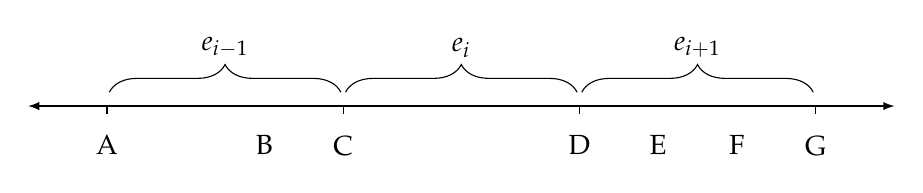
\begin{tikzpicture}
% axis
\draw[latex-latex] (0,0) -- (11,0) ;

% epoch braces
\draw [decorate,decoration={brace,amplitude=10pt} ,yshift=5pt] (1.03,0) -- (3.97,0)
  node [midway, above, yshift=9pt]{$e_{i-1}$};
\draw [decorate,decoration={brace,amplitude=10pt} ,yshift=5pt] (4.03,0) -- (6.97,0)
  node [midway, above, yshift=9pt]{$e_{i}$};
\draw [decorate,decoration={brace,amplitude=10pt} ,yshift=5pt] (7.03,0) -- (9.97,0)
  node [midway, above, yshift=9pt]{$e_{i+1}$};

% epoch boundaries
\foreach \x in  {1,4,7,10}
  \draw[shift={(\x,0)}] (0pt,0pt) -- (0pt,-3pt);

\node at (1,-0.5) {A};
\node at (3,-0.5) {B};
\node at (4,-0.5) {C};
\node at (7,-0.5) {D};
\node at (8,-0.5) {E};
\node at (9,-0.5) {F};
\node at (10,-0.5) {G};

\end{tikzpicture}

We must therefore store the last three stake distributions.
The mnemonic ``mark, set, go'' will be used to keep
track of the snapshots, where the label ``mark'' refers to the most recent snapshot,
and ``go'' refers to the snapshot that is ready to be used in the reward calculation.
In the above diagram, the snapshot taken at (A) is labeled ``mark'' during epoch $e_{i-1}$,
``set'' during epoch $e_i$ and ``go'' during epoch $e_{i+1}$. At (G) the snapshot
taken at (A) is no longer needed and will be discarded.

The two main transition systems in this section are:
\begin{itemize}
  \item The transition system named $\mathsf{EPOCH}$, which is defined in
    Section~\ref{sec:total-epoch}, covers what happens at the epoch boundary,
    such as at (A), (C), (D) and (G).
  \item The transition named $\mathsf{RUPD}$, which is defined in
    Section~\ref{sec:reward-update-trans}, covers the reward calculation that
    happens between (E) and (F).
\end{itemize}


\begin{note}
  Between time D and E we are concerned with chain growth and stability.
  Therefore this duration can be stated as 2k blocks (to state it in slots requires details about
  the particular version of the Ouroboros protocol). The duration between F and G is also 2k blocks.
  Between E and F a single honest block is enough to ensure a random nonce.
\end{note}

\subsection{Helper Functions and Accounting Fields}
\label{sec:stake-dist-helpers}

Figure~\ref{fig:funcs:epoch-helper-rewards} defines four helper functions needed
throughout the rest of the section.

\begin{itemize}
  \item The function $\fun{obligation}$ calculates the the minimal amount of coin needed to
    pay out all deposit refunds, as of the current slot.
  \item The function $\fun{poolRefunds}$ is used to calculate the total refunds
    that must be distributed for stake pools scheduled to retire.
    Note that this calculation takes a slot number corresponding to the epoch boundary slot
    when the calculation is performed.  The returned map maps pool operator hashkeys to the
    refunds, which will ultimately be returned to the registered reward account.
  \item The function $\fun{poolStake}$ filters the stake distribution to one stake pool.
\end{itemize}


%%
%% Figure - Helper Functions for Epoch Rules
%%
\begin{figure}[htb]
  \emph{Total possible refunds}
  \begin{align*}
    & \fun{obligation} \in \PParams \to \StakeCreds \to \StakePools \to \Slot \to \Coin \\
    & \obligation{pp}{stkCreds}{stpools}{cslot} =\\
    & \sum\limits_{(\_ \mapsto s) \in \var{stkCreds}}
      \refund{d_{\mathsf{val}}}{d_{\min}}{\lambda_d}{(\slotminus{cslot}{s})}
      + \sum\limits_{(\_ \mapsto s) \in \var{stpools}}
      \refund{p_{\mathsf{val}}}{p_{\min}}{\lambda_p}{(\slotminus{cslot}{s})} \\
    &
      \begin{array}{lr@{~=~}l}
        \where
          & \dval,~d_{\min},~\lambda_d
          & \fun{keyDeposit}~\var{pp},~\fun{keyMinRefund}~\var{pp},~\fun{keyDecayRate}~\var{pp}
          \\
          & p_{\mathsf{val}},~p_{\min},~\lambda_p
          & \fun{poolDeposit}~\var{pp},~\fun{poolMinRefund}~\var{pp},~\fun{poolDecayRate}~\var{pp}
      \end{array}\\
  \end{align*}
  \emph{Pool refunds}
  \begin{align*}
      & \fun{poolRefunds} \in \PParams \to (\KeyHash_{pool} \mapsto \Epoch) \to \Slot \to
      (\KeyHash_{pool} \mapsto \Coin) \\
      & \poolRefunds{pp}{retiring}{cslot} = \left\{
        \var{hk}\mapsto
          \refund{p_{\mathsf{val}}}{p_{\min}}{\lambda_p}{(\slotminus{cslot}{(\fun{slot}~e)})}
          \mid
          \var{hk}\mapsto e\in\var{retiring}
        \right\}\\
      & \where p_{\mathsf{val}},~p_{\min},~\lambda_p =
          \fun{poolDeposit}~\var{pp},~\fun{poolMinRefund}~\var{pp},~\fun{poolDecayRate}~\var{pp} \\
  \end{align*}

  \emph{Filter Stake to one Pool}
  \begin{align*}
      & \fun{poolStake} \in \KeyHash_{pool} \to (\KeyHash_{stake} \mapsto \KeyHash_{pool})
        \to \Stake \to \Stake \\
      & \poolStake{hk}{delegs}{stake} =
        \dom{(\var{delegs}\restrictrange\{hk\})\restrictdom\var{stake}}
  \end{align*}

  \caption{Helper Functions used in Rewards and Epoch Boundary}
  \label{fig:funcs:epoch-helper-rewards}
\end{figure}


The Figure~\ref{fig:defs:accounting} lists the accounting fields, denoted by $\Acnt$,
which will be used throughout this section. It consists of:
\begin{itemize}
  \item The value $\var{treasury}$ tracks the amount of coin currently stored in the treasury.
    Initially there will be no way to remove these funds.
  \item The value $\var{reserves}$ tracks the amount of coin currently stored in the reserves.
    This pot is used to pay rewards.
\end{itemize}
More will be said about the general accounting system in Section~\ref{sec:reward-calc}.

%%
%% Figure - Accounting fields
%%
\begin{figure}[htb]
  \emph{Accounting Fields}
  \begin{equation*}
    \Acnt =
    \left(
      \begin{array}{r@{~\in~}ll}
        \var{treasury} & \Coin & \text{treasury pot}\\
        \var{reserves} & \Coin & \text{reserve pot}\\
      \end{array}
    \right)
  \end{equation*}
  %
  \caption{Accounting fields}
  \label{fig:defs:accounting}
\end{figure}


\subsection{Stake Distribution Calculation}
\label{sec:stake-dist-calc}

This section defines the stake distribution calculations.
Figure~\ref{fig:epoch-defs} introduces three new derived types:
\begin{itemize}
  \item $\type{BlocksMade}$ represents the number of blocks each stake pool produced
    during an epoch.
  \item $\type{Stake}$ represents the amount of stake (in $\type{Coin}$) controlled by each
    stake pool.
\end{itemize}

%%
%% Figure - Epoch Abstract Types
%%
\begin{figure}[htb]
  \emph{Derived types}
  %
  \begin{equation*}
    \begin{array}{r@{~\in~}l@{\qquad=\qquad}lr}
      \var{blocks}
      & \BlocksMade
      & \KeyHash_{pool} \mapsto \N
      & \text{blocks made by stake pools} \\
      \var{stake}
      & \Stake
      & \Credential \mapsto \Coin
      & \text{stake} \\
    \end{array}
  \end{equation*}
  \caption{Epoch definitions}
  \label{fig:epoch-defs}
\end{figure}

The stake distribution calculation is given in Figure~\ref{fig:functions:stake-distribution}.

\begin{itemize}
\item $\fun{aggregate_{+}}$ takes a relation on $A\times B$, where $B$ is any
  monoid $(B,+,e)$ and returns a map from each $a\in A$ to the ``sum'' (using
  the monoidal $+$ operation) of all $b\in B$ such that $(a, b)\in A\times B$.
\item $\fun{stakeDistr}$ uses the $\fun{aggregate_{+}}$ function and several relations to
    compute the stake distribution, mapping each hashkey to the total coin under its control.
    Keys that are not both registered and delegated are filtered out.
    The relation passed to $\fun{aggregate_{+}}$ is made up of:
    \begin{itemize}
      \item $\fun{stakeCred_b}^{-1}$, relating credentials to (base) addresses
      \item $\left(\fun{addrPtr}\circ\var{ptr}\right)^{-1}$, relating credentials to (pointer)
        addresses
      \item $\range{utxo}$, relating addresses to coins
      \item $\fun{stakeCred_r}^{-1}\circ\var{rewards}$, relating (reward) addresses to coins
    \end{itemize}
    The notation for relations is explained in Section~\ref{sec:notation-shelley}.
\end{itemize}

%%
%% Figure Functions for Stake Distribution
%%
\begin{figure}[htb]
  \emph{Aggregation (for a monoid B)}
  %
  \begin{align*}
      & \fun{aggregate_{+}} \in \powerset{(A \times B)} \to (A\mapsto B) \\
      & \fun{aggregate_{+}}~\var{R} = \left\{a\mapsto \sum_{(a,b)\in\var{R}}b
          ~\mid~a\in\dom\var{R}\right\} \\
  \end{align*}
  %
  \emph{Stake Distribution (using functions and maps as relations)}
  %
  \begin{align*}
      & \fun{stakeDistr} \in \UTxO \to \DState \to \PState \to \Stake \\
      & \fun{stakeDistr}~{utxo}~{dstate}~{pstate} =
      (\dom{\var{activeDelegs}})\restrictdom\left(\fun{aggregate_{+}}~\var{stakeRelation}\right)\\
      & \where \\
      & ~~~~ (\var{stkCreds},~\var{rewards},~\var{delegations},~\var{ptrs},~\wcard,~\wcard)
        = \var{dstate} \\
      & ~~~~ (\var{stpools},~\wcard,~\wcard) = \var{pstate} \\
      & ~~~~ \var{stakeRelation} = \left(
        \left(\fun{stakeCred_b}^{-1}\cup\left(\fun{addrPtr}\circ\var{ptr}\right)^{-1}\right)
        \circ\left(\range{\var{utxo}}\right)
        \right)
        \cup \left(\fun{stakeCred_r}^{-1}\circ\var{rewards}\right) \\
      & ~~~~ \var{activeDelegs} =
               (\dom{stkCreds}) \restrictdom \var{delegations} \restrictrange (\dom{stpools}) \\
  \end{align*}

  \caption{Stake Distribution Function}
  \label{fig:functions:stake-distribution}
\end{figure}

\clearpage

\subsection{Snapshot Transition}
\label{sec:snapshots}

The state transition types for stake distribution snapshots are given in
Figure~\ref{fig:ts-types:snapshot}.
Each snapshot consists of:
\begin{itemize}
  \item $\var{stake}$, a stake distribution, which is defined in
    Figure~\ref{fig:epoch-defs} as a mapping of credentials to coin.
  \item $\var{delegations}$, a delegation map, mapping credentials to stake pools.
  \item $\var{poolParameters}$, storing the pool parameters of each stake pool.
\end{itemize}

The type $\type{\Snapshots}$ contains the
information needing to be saved on the epoch boundary:
\begin{itemize}
  \item $\var{pstake_{mark}}$, $\var{pstake_{set}}$ and $\var{pstake_{go}}$ are the three
    snapshots as explained in Section~\ref{sec:reward-overview}.
  \item $\var{feeSS}$ stores the fees and decayed deposit amounts at the epoch boundary.
\end{itemize}

%%
%% Figure - Snapshots Defs
%%
\begin{figure}[htb]
  \emph{Snapshot environment}
  \begin{equation*}
    \SnapshotEnv =
    \left(
      \begin{array}{r@{~\in~}ll}
        \var{pp} & \PParams & \text{protocol parameters}\\
        \var{dstate} & \DState & \text{delegation state}\\
        \var{pstate} & \PState & \text{pool state}\\
      \end{array}
    \right)
  \end{equation*}
  %
  \emph{Snapshots}
  \begin{equation*}
    \Snapshot =
    \left(
      \begin{array}{r@{~\in~}ll}
        \var{stake} & \Stake & \text{stake distribution}\\
        \var{delegations} & \Credential\mapsto\KeyHash_{pool}
                          & \text{stake delegations}\\
        \var{poolParameters} & \KeyHash_{pool} \mapsto \PoolParam & \text{pool parameters }\\
      \end{array}
    \right)
  \end{equation*}

  \begin{equation*}
    \Snapshots =
    \left(
      \begin{array}{r@{~\in~}ll}
        \var{pstake_{mark}} & \Snapshot & \text{newest stake}\\
        \var{pstake_{set}}  & \Snapshot & \text{middle stake}\\
        \var{pstake_{go}}   & \Snapshot & \text{oldest stake}\\
        \var{feeSS} & \Coin & \text{fee snapshot}\\
      \end{array}
    \right)
  \end{equation*}
  %
  \emph{Snapshot States}
  \begin{equation*}
    \SnapshotState =
    \left(
      \begin{array}{r@{~\in~}ll}
        \var{ss} & \Snapshots & \text{snapshots}\\
        \var{utxoSt} & \UTxOState & \text{utxo state}\\
      \end{array}
    \right)
  \end{equation*}
  %
  \emph{Snapshot transitions}
  \begin{equation*}
    \_ \vdash
    \var{\_} \trans{snap}{\_} \var{\_}
    \subseteq \powerset (\SnapshotEnv \times \SnapshotState \times \Epoch \times \SnapshotState)
  \end{equation*}
  %
  \caption{Snapshot transition-system types}
  \label{fig:ts-types:snapshot}
\end{figure}

The snapshot transition rule is given in Figure~\ref{fig:rules:snapshot}.
This transition has no preconditions and results in the following state change:

\begin{itemize}
  \item The oldest snapshot is replaced with the penultimate one.
  \item The penultimate snapshot is replaced with the newest one.
  \item The newest snapshot is replaced with one just calculated.
  \item The fees and decayed deposits are stored in $\var{feeSS}$. Note that this value will not
    change between epochs, unlike the $\var{fees}$ and $\var{deposits}$ values in the UTxO state.
  \item In the UTxO state, the decayed deposit amounts are moved from the deposit pot
    to the fee pool. Note that in the reward transition (Section~\ref{sec:reward-calc}),
    the value $\var{feeSS}$ will be removed from the fee pot in the UTxO state.
    The decay is calculated based on \textit{the first slot in the upcoming epoch}.
\end{itemize}

%%
%% Figure - Snapshot Rule
%%
\begin{figure}[htb]
  \begin{equation}\label{eq:snapshot}
    \inference[Snapshot]
    {
      {
      \begin{array}{r@{~\leteq~}l}
        (\var{stkCreds},~\wcard,~\var{delegations},~\wcard,~\wcard,~\wcard) & \var{dstate}\\
        (\var{stpools},~\var{poolParams},~\wcard) & \var{pstate}\\
        \var{stake} & \stakeDistr{utxo}{dstate}{pstate} \\
        \var{slot} & \firstSlot{e} \\
        \var{oblg} & \obligation{pp}{stkCreds}{stpools}{slot} \\
        \var{decayed} & \var{deposits} - \var{oblg} \\
      \end{array}
      }
    }
    {
      \begin{array}{r}
        \var{pp} \\
        \var{dstate} \\
        \var{pstate} \\
      \end{array}
      \vdash
      \left(
        \begin{array}{r}
          \var{pstake_{mark}}\\
          \var{pstake_{set}}\\
          \var{pstake_{go}}\\
          \var{feeSS} \\
          ~ \\
          \var{utxo} \\
          \var{deposits} \\
          \var{fees} \\
          \var{pup} \\
        \end{array}
      \right)
      \trans{snap}{e}
      \left(
        \begin{array}{r}
          \varUpdate{(\var{stake},~\var{delegations},~\var{poolParams})} \\
          \varUpdate{\var{pstake_{mark}}} \\
          \varUpdate{\var{pstake_{set}}} \\
          \varUpdate{\var{fees} + \var{decayed}} \\
          ~ \\
          \var{utxo} \\
          \varUpdate{\var{oblg}} \\
          \varUpdate{\var{fees} + \var{decayed}} \\
          \var{pup} \\
        \end{array}
      \right)
    }
  \end{equation}
  \caption{Snapshot Inference Rule}
  \label{fig:rules:snapshot}
\end{figure}

\clearpage

\subsection{Pool Reaping Transition}
\label{sec:pool-reap}

Figure~\ref{fig:ts-types:pool-reap} defines the types for the pool reap transition,
which is responsible for removing pools slated for retirement in the given epoch.

%%
%% Figure - Pool Reap Defs
%%
\begin{figure}[htb]
  \emph{Pool Reap State}
  \begin{equation*}
    \PlReapState =
    \left(
      \begin{array}{r@{~\in~}ll}
        \var{utxoSt} & \UTxOState & \text{utxo state}\\
        \var{acnt} & \Acnt & \text{accounting}\\
        \var{dstate} & \DState & \text{delegation state}\\
        \var{pstate} & \PState & \text{pool state}\\
      \end{array}
    \right)
  \end{equation*}
  %
  \emph{Pool Reap transitions}
  \begin{equation*}
    \_ \vdash \_ \trans{poolreap}{\_} \_ \in
    \powerset (\PParams \times \PlReapState \times \Epoch \times \PlReapState)
  \end{equation*}
  %
  \caption{Pool Reap Transition}
  \label{fig:ts-types:pool-reap}
\end{figure}


The pool-reap transition rule is given in Figure~\ref{fig:rules:pool-reap}.
This transition has no preconditions and results in the following state change:

\begin{itemize}
  \item For each retiring pool, the refund for the pool registration deposit is added to the
    pool's registered reward account, provided the reward account is still registered.
  \item The sum of all the refunds attached to unregistered reward accounts are added to the
    treasury.
  \item The deposit pool is reduced by the amount of claimed and unclaimed refunds.
  \item Any delegation to a retiring pool is removed.
  \item Each retiring pool is removed from all four maps in the pool state.
\end{itemize}

%%
%% Figure - Pool Reap Rule
%%
\begin{figure}[htb]
  \begin{equation}\label{eq:pool-reap}
    \inference[Pool-Reap]
    {
      {
      \begin{array}{r@{~\leteq~}l}
        \var{retired} & \dom{(\var{retiring}^{-1}~\var{e})} \\
        \var{pr} & \poolRefunds{pp}{(\var{retired}\restrictdom\var{stpools})}{(\firstSlot{e})} \\
        \var{rewardAcnts}
                 & \{\var{hk}\mapsto \fun{poolRAcnt}~\var{pool} \mid
                   \var{hk}\mapsto\var{pool} \in \var{retired}\restrictdom\var{poolParams} \} \\
        \var{rewardAcnts'} & \left\{
                        a \mapsto c
                        \mathrel{\Bigg|}
                        \begin{array}{r@{~\in~}l}
                          \var{hk} \mapsto c & \var{pr}, \\
                          \var{hk}\mapsto\var{a} & \var{rewardAcnts} \\
                        \end{array}
                      \right\} \\
        \var{refunds} & \dom{rewards}\restrictdom\var{rewardAcnts'} \\
        \var{mRefunds} & \dom{rewards}\subtractdom\var{rewardAcnts'} \\
        \var{refunded} & \sum\limits_{\wcard\mapsto c\in\var{refunds}} c \\
        \var{unclaimed} & \sum\limits_{\wcard\mapsto c\in\var{mRefunds}} c \\
      \end{array}
      }
    }
    {
      \var{pp}
      \vdash
      \left(
        \begin{array}{r}
          \var{utxo} \\
          \var{deposits} \\
          \var{fees} \\
          \var{ups} \\
          ~ \\
          \var{treasury} \\
          \var{reserves} \\
          ~ \\
          \var{stkCreds} \\
          \var{rewards} \\
          \var{delegations} \\
          \var{ptrs} \\
          \var{genDelegs} \\
          \var{i_{rwd}} \\
          ~ \\
          \var{stpools} \\
          \var{poolParams} \\
          \var{retiring} \\
        \end{array}
      \right)
      \trans{poolreap}{e}
      \left(
        \begin{array}{rcl}
          \var{utxo} \\
          \varUpdate{\var{deposits}}
          & \varUpdate{-}
          & \varUpdate{(\var{unclaimed} + \var{refunded})} \\
          \var{fees} \\
          \var{ups} \\
          ~ \\
          \varUpdate{\var{treasury}} & \varUpdate{+} & \varUpdate{\var{unclaimed}} \\
          \var{reserves} \\
          ~ \\
          \var{stkCreds} \\
          \varUpdate{\var{rewards}} & \varUpdate{\unionoverridePlus} & \varUpdate{\var{refunds}} \\
          \varUpdate{\var{delegations}} & \varUpdate{\subtractrange} & \varUpdate{\var{retired}} \\
          \var{ptrs} \\
          \var{genDelegs} \\
          \var{i_{rwd}}\\
          ~ \\
          \varUpdate{\var{retired}} & \varUpdate{\subtractdom} & \varUpdate{\var{stpools}} \\
          \varUpdate{\var{retired}} & \varUpdate{\subtractdom} & \varUpdate{\var{poolParams}} \\
          \varUpdate{\var{retired}} & \varUpdate{\subtractdom} & \varUpdate{\var{retiring}} \\
        \end{array}
      \right)
    }
  \end{equation}
  \caption{Pool Reap Inference Rule}
  \label{fig:rules:pool-reap}
\end{figure}

\clearpage

\subsection{Protocol Parameters Update Transition}
\label{sec:pparam-update}

Finally, reaching the epoch boundary may trigger a change in the protocol
parameters. The protocol parameters environment consists of the new
protocol parameters and the delegation and pool states.
The state change is a change of the $\UTxOState$, the $\Acnt$ states and the current $\PParams$.
The type of this state transition is given in Figure~\ref{fig:ts-types:new-proto-param}.

%%
%% Figure - New Proto Param Defs
%%
\begin{figure}[htb]
  \emph{New Proto Param environment}
  \begin{equation*}
    \NewPParamEnv =
    \left(
      \begin{array}{r@{~\in~}ll}
        \var{pp_{new}} & \PParams^? & \text{new protocol parameters}\\
        \var{dstate} & \DState & \text{delegation state}\\
        \var{pstate} & \PState & \text{pool state}\\
      \end{array}
    \right)
  \end{equation*}
  %
  \emph{New Proto Param States}
  \begin{equation*}
    \NewPParamState =
    \left(
      \begin{array}{r@{~\in~}ll}
        \var{utxoSt} & \UTxOState & \text{utxo state}\\
        \var{acnt} & \Acnt & \text{accounting}\\
        \var{pp} & \PParams & \text{current protocol parameters}\\
      \end{array}
    \right)
  \end{equation*}
  %
  \emph{New Proto Param transitions}
  \begin{equation*}
    \_ \vdash
    \var{\_} \trans{newpp}{\_} \var{\_}
    \subseteq \powerset (\NewPParamEnv \times \NewPParamState \times \Epoch \times \NewPParamState)
  \end{equation*}
  %
  \caption{New Proto Param transition-system types}
  \label{fig:ts-types:new-proto-param}
\end{figure}


Figure~\ref{fig:rules:new-proto-param} defines the new protocol parameter transition.
The transition has two rules, depending on whether or not the new protocol parameters
meet some requirements.
In particular, we require that the new parameters would not incur a debt of the system that
can not be covered by the reserves, and that the max block size is greater than the sum of the
max transaction size and the max header size.
If the requirements are met, the new protocol parameters are accepted, the proposal is reset,
and the reserves are adjusted to account for changes in the deposits.
Otherwise, the only change is that the proposal is reset.

Regarding adjusting the reserves for changes in the deposits, one of three things happens:

\begin{itemize}
  \item If the new protocol parameters mean that \textbf{fewer} funds are required in the
    deposit pot to cover all possible refunds, then the excess is moved to the reserves.

  \item If the new protocol parameters mean that \textbf{more} funds are required in the
    deposit pot to cover all possible refunds and the difference is \textbf{less} than
    the reserve pot, then funds are moved from the reserve pot to cover the difference.

  \item If the new protocol parameters mean that \textbf{more} funds are required in the
    deposit pot to cover all possible refunds and the difference is \textbf{more} than
    the reserve pot, then Rule~\ref{eq:new-pc-denied} meets the precondition and the
    only change of state is that the update proposals are reset.
\end{itemize}

Note that here, unlike most of the inference rules in this document,
the $\var{utxoSt'}$ and the $\var{acnt'}$ do not come from valid UTxO or
accounts transitions in the antecedent. We simply define the consequent
transition using these directly (instead of listing all the fields in both
states in the consequent transition). It is done this way here
for ease of reading.

%%
%% Figure - New Proto Param Rule
%%
\begin{figure}[htb]
  \begin{equation}\label{eq:new-pc-accepted}
    \hspace{-0.3cm}
    \inference[New-Proto-Param-Accept]
    {
      \var{pp_{new}}\neq\Nothing \\~\\
      {\begin{array}{rcl}
         \var{slot} & \leteq & \firstSlot{e} \\
         \var{oblg_{cur}} & \leteq & \obligation{pp}{stkCreds}{stpools}{slot} \\
         \var{oblg_{new}} & \leteq & \obligation{pp_{new}}{stkCreds}{stpools}{slot} \\
         \var{(\wcard,~\wcard,~\wcard,~\wcard,~\wcard,~\wcard,~\var{i_{rwd}})} &
                                                                                      \leteq
                              & \var{dstate}\\
         \var{diff} & \leteq & \var{oblg_{cur}} - \var{oblg_{new}}\\
         (\var{utxo},~\var{deposits},~\var{fees},~\var{ups}) & \leteq & \var{utxoSt} \\
         (\var{pup},~\var{aup},~\var{favs},~\var{avs}) & \leteq & \var{ups} \\
      \end{array}}
      \\~\\~\\
      \var{oblg_{cur}} = \var{deposits} \\
      \var{reserves} + \var{diff} \geq \sum\limits_{\wcard\mapsto\var{val}\in\var{i_{rwd}}} val \\
      \fun{maxTxSize}~\var{pp_{new}} + \fun{maxHeaderSize}~\var{pp_{new}} <
        \fun{maxBlockSize}~\var{pp_{new}}
      \\~\\
        \var{utxoSt'} \leteq
        \left(\var{utxo},~\varUpdate{oblg_{new}},~\var{fees}
        \left(\varUpdate{\emptyset},~\var{aup},~\var{favs},~\var{avs}\right)\right)
      \\~\\
      (\var{treasury},~\var{reserves})\leteq \var{acnt} \\
      \var{acnt'} \leteq (\var{treasury},~\varUpdate{reserves + diff}) \\
    }
    {
      \begin{array}{l}
        \var{pp_{new}}\\
        \var{dstate}\\
        \var{pstate}\\
      \end{array}
      \vdash
      \left(
        \begin{array}{r}
          \var{utxoSt} \\
          \var{acnt} \\
          \var{pp}
        \end{array}
      \right)
      \trans{newpp}{e}
      \left(
        \begin{array}{rcl}
          \varUpdate{utxoSt'}\\
          \varUpdate{acnt'} \\
          \varUpdate{\var{pp_{new}}} \\
        \end{array}
      \right)
    }
  \end{equation}

  \nextdef

  \begin{equation}\label{eq:new-pc-denied}
    \inference[New-Proto-Param-Denied]
    {
      \left({\begin{array}{c}
            \var{pp_{new}}=\Nothing \\
        \lor \\
        \var{reserves} + \var{diff} < \sum\limits_{\wcard\mapsto\var{val}\in\var{i_{rwd}}} val\\
        \lor \\
        \fun{maxTxSize}~\var{pp_{new}} + \fun{maxHeaderSize}~\var{pp_{new}} \geq
          \fun{maxBlockSize}~\var{pp_{new}}
      \end{array}}\right)
      \\~\\~\\
      {\begin{array}{rcl}
          \var{slot} & \leteq & \firstSlot{e} \\
          \var{oblg_{cur}} & \leteq & \obligation{pp}{stkCreds}{stpools}{slot} \\
          \var{oblg_{new}} & \leteq & \obligation{pp_{new}}{stkCreds}{stpools}{slot} \\
         \var{(\wcard,~\wcard,~\wcard,~\wcard,~\wcard,~\wcard,~\var{i_{rwd}})} &
                                                                                 \leteq
                              & \var{dstate}\\
         \var{diff} & \leteq & \var{oblg_{cur}} - \var{oblg_{new}}
      \end{array}}
      \\~\\~\\
      \left(\var{utxo},~\var{oblg},~\var{fees}
        \left(\var{pup},~\var{aup},~\var{favs},~\var{avs}\right)\right)
        \leteq \var{utxoSt} \\
        \var{utxoSt'} \leteq
        \left(\var{utxo},~\var{oblg},~\var{fees}
        \left(\varUpdate{\emptyset},~\var{aup},~\var{favs},~\var{avs}\right)\right)
    }
    {
      \begin{array}{l}
        \var{pp_{new}}\\
        \var{dstate}\\
        \var{pstate}\\
      \end{array}
      \vdash
      \left(
        \begin{array}{r}
          \var{utxoSt} \\
          \var{acnt} \\
          \var{pp}
        \end{array}
      \right)
      \trans{newpp}{e}
      \left(
        \begin{array}{rcl}
          \varUpdate{utxoSt'}\\
          \var{acnt} \\
          \var{pp}
        \end{array}
      \right)
    }
  \end{equation}
  \caption{New Proto Param Inference Rule}
  \label{fig:rules:new-proto-param}
\end{figure}

\clearpage

\subsection{Complete Epoch Boundary Transition}
\label{sec:total-epoch}

Finally, it is possible to define the complete epoch boundary transition type,
which is defined in Figure~\ref{fig:ts-types:epoch}.
The transition has no evironment.
The state is made up of the the accounting state, the snapshots, the ledger state and the
protocol parameters.
The transition uses a helper function $\fun{votedValue}$ which returns
the consensus value of update proposals in the event that consensus is met.
\textbf{Note that} $\fun{votedValue}$
\textbf{is only well-defined if } $\Quorum$
\textbf{is greater than half the number of core nodes, i.e.}
$\Quorum > |\var{genDelegs}|/2$ \textbf{.}

%%
%% Figure - Epoch Defs
%%
\begin{figure}[htb]
  \emph{Epoch States}
  \begin{equation*}
    \EpochState =
    \left(
      \begin{array}{r@{~\in~}ll}
        \var{acnt} & \Acnt & \text{accounting}\\
        \var{ss} & \Snapshots & \text{snapshots}\\
        \var{ls} & \LState & \text{ledger state}\\
        \var{prevPp} & \PParams & \text{previous protocol parameters}\\
        \var{pp} & \PParams & \text{protocol parameters}\\
      \end{array}
    \right)
  \end{equation*}
  %
  \emph{Epoch transitions}
  \begin{equation*}
    \vdash
    \var{\_} \trans{epoch}{\_} \var{\_}
    \subseteq \powerset (\EpochState \times \Epoch \times \EpochState)
  \end{equation*}
  %
  \emph{Accessor Functions}
  \begin{equation*}
    \begin{array}{r@{~\in~}lr}
      \fun{getIR} & \EpochState \to (\StakeCredential \mapsto \Coin)
                  & \text{get instantaneous rewards} \\
    \end{array}
  \end{equation*}
  %
  \emph{Helper Functions}
  \begin{align*}
      & \fun{votedValue} \in (\KeyHashGen\mapsto\PParamsUpdate) \to \PParamsUpdate^?\\
      & \fun{votedValue}~\var{vs} =
        \begin{cases}
          p & \exists p\in\range{vs}~(|vs\restrictrange p|\geq \Quorum) \\
          \Nothing & \text{otherwise} \\
        \end{cases}
  \end{align*}
  %
  \caption{Epoch transition-system types}
  \label{fig:ts-types:epoch}
\end{figure}


The epoch transition rule calls $\mathsf{SNAP}$, $\mathsf{POOLREAP}$ and $\mathsf{NEWPP}$
in sequence. It also stores the previous protocol parameters in $\var{prevPp}$.
The previous protocol parameters will be used for the reward calculation in the upcoming epoch,
note that they correspond to the epoch for which the rewards are being calculated.
Additionally, this transition also adopts the pool parameters $\var{fPoolParams}$
corresponding to the pool re-registration certificates which we submitted late in the ending epoch.
The ordering of these rules is important.
The stake pools which will be updated by $\var{fPoolParams}$ or
reaped during the $\mathsf{POOLREAP}$ transition must still be a
part of the new snapshot, and so $\mathsf{SNAP}$ must occur before these two actions.
Moreover, $\mathsf{SNAP}$ sets the deposit pot equal to current obligation,
which is a property that is preserved by $\mathsf{POOLREAP}$ and which
is necessary for the preservation of Ada property in the $ \mathsf{NEWPP}$ transition.

%%
%% Figure - Epoch Rule
%%
\begin{figure}[htb]
  \begin{equation}\label{eq:epoch}
    \inference[Epoch]
    {
      (\var{utxoSt},~(\var{dstate},~\var{pstate}))\leteq\var{ls} \\
      {
        \begin{array}{r}
          \var{pp}\\
          \var{dstate} \\
          \var{pstate} \\
        \end{array}
      }
      \vdash
      {
        \left(
          {
            \begin{array}{r}
              \var{ss} \\
              \var{utxoSt} \\
            \end{array}
          }
        \right)
      }
      \trans{\hyperref[fig:rules:snapshot]{snap}}{e}
      {
        \left(
          {
            \begin{array}{r}
              \var{ss'} \\
              \var{utxoSt'} \\
            \end{array}
          }
        \right)
      }
      \\~\\~\\
      (\var{stpools},~\var{poolParams},~\var{fPoolParams},~\var{retiring})\leteq\var{pstate}
      \\
      \var{pstate'}\leteq(\var{stpools},~\var{poolParams}\unionoverrideRight\var{fPoolParams},
      ~\emptyset,~\var{retiring})
      \\~\\~\\
      \var{pp}
      \vdash
      \left(
        {
          \begin{array}{r}
            \var{utxoSt'} \\
            \var{acnt} \\
            \var{dstate} \\
            \var{pstate'} \\
          \end{array}
        }
      \right)
      \trans{\hyperref[fig:rules:pool-reap]{poolreap}}{e}
      \left(
      {
        \begin{array}{rcl}
            \var{utxoSt''} \\
            \var{acnt'} \\
            \var{dstate'} \\
            \var{pstate''} \\
        \end{array}
      }
      \right)
      \\~\\~\\
      \var{(\wcard,~\wcard,~\wcard,~\var{pup})}\leteq\var{utxoSt'}\\
      \var{pp_{new}}\leteq\var{pp}\unionoverrideRight
      \fun{votedValue}~\var{pup}\\
      {
        \begin{array}{r}
          \var{pp_{new}}\\
          \var{dstate'}\\
          \var{pstate''}\\
        \end{array}
      }
      \vdash
      \left(
        {
          \begin{array}{r}
            \var{utxoSt''} \\
            \var{acnt'} \\
            \var{pp}\\
          \end{array}
        }
      \right)
      \trans{\hyperref[fig:rules:new-proto-param]{newpp}}{e}
      \left(
      {
        \begin{array}{rcl}
            \var{utxoSt'''} \\
            \var{acnt''} \\
            \var{pp'}\\
        \end{array}
      }
      \right)
      \\~\\~\\
      \var{ls}' \leteq (\var{utxoSt}''',~(\var{dstate}',~\var{pstate}''))
    }
    {
      \vdash
      \left(
      \begin{array}{r}
        \var{acnt} \\
        \var{ss} \\
        \var{ls} \\
        \var{prevPp} \\
        \var{pp} \\
      \end{array}
      \right)
      \trans{epoch}{e}
      \left(
      \begin{array}{rcl}
        \varUpdate{\var{acnt''}} \\
        \varUpdate{\var{ss'}} \\
        \varUpdate{\var{ls'}} \\
        \varUpdate{\var{pp}} \\
        \varUpdate{\var{pp'}} \\
      \end{array}
      \right)
    }
  \end{equation}
  \caption{Epoch Inference Rule}
  \label{fig:rules:epoch}
\end{figure}

\clearpage

\subsection{Rewards Distribution Calculation}
\label{sec:reward-dist}

This section defines the reward calculation for the proof of stake leader election.
Figure~\ref{fig:functions:rewards} defines the pool reward as described in section
5.5.2 of~\cite{delegation_design}.

\begin{itemize}
  \item The function $\fun{maxPool}$ gives the maximum reward a stake pool can receive in an epoch.
    This is a fraction of the total available rewards for the epoch.
    The result depends on the pool's relative stake, the pool's pledge and the following
    protocol parameters:
    \begin{itemize}
      \item $\var{a_0}$, the leader-stake influence
      \item $n_{opt}$, the optimal number of saturated stake pools
    \end{itemize}
  \item The function $\fun{poolReward}$ gives the total rewards available to be
    distributed to the members of the given pool. It depends on the protocol parameter $d$,
    the relative stake $\sigma$, the number $n$ of blocks the pool added to the chain and the
    total number $\overline{N}$ of blocks added to the chain in the last epoch.

\end{itemize}

%%
%% Figure - Functions for the Reward Calculation
%%
\begin{figure}[htb]
  \emph{Maximal Reward Function, called $f(s,\sigma)$ in section 5.5.2 of~\cite{delegation_design}}
  %
  \begin{align*}
      & \fun{maxPool} \in \PParams \to \Coin \to \unitInterval \to \unitInterval \to \Coin \\
      & \fun{maxPool}~\var{pp}~\var{R}~\sigma~\var{p_r} =
          ~~~\floor*{
             \frac{R}{1 + a_0}
             \cdot
             \left(
               \sigma' + p'\cdot a_0\cdot\frac{\sigma' - p'\frac{z_0-\sigma'}{z_0}}{z_0}
             \right)} \\
      & ~~~\where \\
      & ~~~~~~~a_0 = \fun{influence}~pp \\
      & ~~~~~~~n_{opt} = \fun{nopt}~pp \\
      & ~~~~~~~z_0 = 1/n_{opt} \\
      & ~~~~~~~\sigma'=\min(\sigma,~z_0) \\
      & ~~~~~~~p'=\min(p_r,~z_0) \\
  \end{align*}

  \emph{Actual Reward Function, called $\hat{f}$ in section 5.5.2 of~\cite{delegation_design}}
  %
  \begin{align*}
      & \fun{poolReward} \in \unitInterval \to \unitInterval \to \N \to \N \to \Coin \to \Coin \\
      & \poolReward{d}{\sigma}{n}{\overline{N}}{f} =
      \floor*{\overline{p}\cdot\var{f}}\\
      & ~~~\where \\
      & ~~~~~~~\overline{p} =
        \begin{cases}
          \frac{\beta}{\sigma} & \text{if } d < 0.8 \\
          1 & \text{otherwise}
        \end{cases} \\
      & ~~~~~~~\beta = \frac{n}{\max(1, \overline{N})} \\
  \end{align*}
  \caption{Functions used in the Reward Calculation}
  \label{fig:functions:rewards}
\end{figure}

\clearpage

Figure~\ref{fig:functions:reward-splitting} gives the calculation for
splitting the pool rewards with its members, as described in 6.5.2 of \cite{delegation_design}.
The portion of rewards allocated to the pool operator and owners is different
than that of the members.

\begin{itemize}
  \item The $\fun{r_{operator}}$ function calculates the leader reward, based on the pool cost,
    margin and the proportion of the pool's total stake.  Note that this reward will go to the
    reward account specified in the pool registration certificate.
  \item The $\fun{r_{member}}$ function calculates the member reward, proportionally to their
    stake after the cost and margin are removed.
\end{itemize}

%%
%% Figure - Functions for the Reward Splitting
%%
\begin{figure}[htb]
  \emph{Pool leader reward, from section 5.5.3 of \cite{delegation_design}}
  %
  \begin{align*}
      & \fun{r_{operator}} \in \Coin \to \PoolParam \to \unitInterval \to \unitIntervalNonNull \to \Coin \\
      & \lReward{\hat{f}}{pool}{s}{\sigma} =
        \begin{cases}
        \hat{f} & \hat{f} \leq c\\
        c + \floor*{(\hat{f} - c)\cdot\left(m + (1-m)\cdot\frac{s}{\sigma}\right) }&
        \text{otherwise.}
      \end{cases} \\
      & ~~~\where \\
      & ~~~~~~~c = \fun{poolCost}~pool \\
      & ~~~~~~~m = \fun{poolMargin}~pool \\
  \end{align*}

  \emph{Pool member reward, from section 5.5.3 of \cite{delegation_design}}
  %
  \begin{align*}
    & \fun{r_{member}} \in \Coin \to \PoolParam \to \unitInterval \to \unitIntervalNonNull \to \Coin \\
    & \mReward{\hat{f}}{pool}{t}{\sigma} =
      \begin{cases}
        0 & \hat{f} \leq c\\
        \floor*{(\hat{f} - c)\cdot(1-m)\cdot\frac{t}{\sigma}} &
        \text{otherwise.}
      \end{cases} \\
    & ~~~\where \\
    & ~~~~~~~c = \fun{poolCost}~pool \\
    & ~~~~~~~m = \fun{poolMargin}~pool \\
  \end{align*}

  \caption{Functions used in the Reward Splitting}
  \label{fig:functions:reward-splitting}
\end{figure}


Finally, the full reward calculation is presented in Figure~\ref{fig:functions:reward-calc}.
The calculation is done pool-by-pool.
\begin{itemize}
\item The $\fun{rewardOnePool}$ function calculates the rewards given out to
  each member of a given pool. The pool leader is identified by the stake
  credential of the pool operator. The function returns the rewards, calculated
  as follows:
    \begin{itemize}
      \item $\var{pstake}$, the total amount of stake controlled by the stake pool.
      \item $\var{ostake}$, the total amount of stake controlled by the stake pool operator
        and owners
      \item $\sigma$, the total proportion of stake controlled by the stake pool.
      \item $\overline{N}$, the expected number of blocks the pool should have produced.
      \item $\var{pledge}$, the pool's pledge in lovelace.
      \item $p_r$, the pool's pledge, as a proportion of active stake.
      \item $\var{maxP}$, maximum rewards the pool can claim if the pledge is met,
        and zero otherwise.
      \item $\var{poolR}$, the pool's actual reward, based on its performance.
      \item $\var{mRewards}$, the member's rewards as a mapping of reward accounts to coin.
      \item $\var{lReward}$, the leader's reward as coin.
      \item $\var{potentialRewards}$, the combination of $\var{mRewards}$ and $\var{lRewards}$.
      \item $\var{rewards}$, the restriction of $\var{potentialRewards}$ to the active
        reward accounts.
    \end{itemize}
  \item The $\fun{reward}$ function applies $\fun{rewardOnePool}$ to each registered stake pool.
\end{itemize}

%%
%% Figure - The Reward Calculation
%%
\begin{figure}[htb]
  \emph{Calculation to reward a single stake pool}
  %
  \begin{align*}
    & \fun{rewardOnePool} \in \PParams \to \Coin \to \N \to \N \to \KeyHash \to \PoolParam\\
      & ~~~\to \Stake \to \Coin \to \powerset{\AddrRWD}
           \to (\AddrRWD \mapsto \Coin) \\
      & \rewardOnePool{pp}{R}{n}{\overline{N}}{poolHK}{pool}{stake}{tot}{addrs_{rew}} =
          \var{rewards}\\
      & ~~~\where \\
      & ~~~~~~~\var{pstake} = \sum_{\_\mapsto c\in\var{stake}} c \\
      & ~~~~~~~\var{ostake} = \sum_{\substack{
        hk_\mapsto c\in\var{stake}\\
        hk\in(\fun{poolOwners}~\var{pool})\\
        }} c \\
      & ~~~~~~~\sigma = \var{pstake} / tot \\
      & ~~~~~~~\var{pledge} = \fun{poolPledge}~pool \\
      & ~~~~~~~p_{r} = \var{pledge} / \var{tot} \\
      & ~~~~~~~maxP =
      \begin{cases}
        \fun{maxPool}~\var{pp}~\var{R}~\sigma~\var{p_r}&
        \var{pledge} \leq \var{ostake}\\
        0 & \text{otherwise.}
      \end{cases} \\
      & ~~~~~~~\var{poolR} = \poolReward{(\fun{d}~pp)}{\sigma}{n}{\overline{N}}{maxP} \\
      & ~~~~~~~\var{mRewards} = \left\{
                                  \addrRw~hk\mapsto\mReward{poolR}{pool}{\frac{c}{tot}}{\sigma}
                                  ~\Big\vert~
                                  hk\mapsto c\in\var{stake},~~hk \neq\var{poolHK}
                               \right\}\\
      & ~~~~~~~\var{lReward} = \lReward{poolR}{pool}{\frac{\var{ostake}}{tot}}{\sigma} \\
      & ~~~~~~~\var{potentialRewards} =
                 \var{mRewards} \cup
                 \{(\fun{poolRAcnt}~\var{pool})\mapsto\var{lReward}\} \\
      & ~~~~~~~\var{rewards} = \var{addrs_{rew}}\restrictdom{\var{potentialRewards}} \\
  \end{align*}

  \emph{Calculation to reward all stake pools}
  %
  \begin{align*}
      & \fun{reward} \in \PParams \to \BlocksMade \to \Coin\to \powerset{\AddrRWD}
      \to (\KeyHash \mapsto \PoolParam) \\
      & ~~~\to \Stake \to (\KeyHash_{stake} \mapsto \KeyHash_{pool}) \to
      \Coin \to (\AddrRWD \mapsto \Coin)\\
      & \reward{pp}{blocks}{R}{addrs_{rew}}{poolParams}{stake}{delegs}{total}
          = \var{rewards}\\
      & ~~~\where \\
      & ~~~~~~~tot = \sum_{\_\mapsto c\in \var{stake}}c \\
      & ~~~~~~~\var{\overline{N}} = \sum_{\_\mapsto m\in blocks}m \\
      & ~~~~~~~pdata = \left\{
        hk\mapsto \left(p,~n,~\poolStake{hk}{delegs}{stake}\right)
        \mathrel{\Bigg|}
        \begin{array}{r@{\mapsto}c@{~\in~}l}
          hk & \var{p} & \var{poolParams} \\
          hk & \var{n} & \var{blocks} \\
        \end{array}
      \right\} \\
      & ~~~~~~~\var{results} = \left\{
        hk \mapsto \rewardOnePool{pp}{R}{n}{\overline{N}}{hk}{p}{s}{tot}{addrs_{rew}}
                 \mid
        hk\mapsto(p, n, s)\in\var{pdata} \right\} \\
      & ~~~~~~~\var{rewards} = \bigcup_{\wcard\mapsto\var{r}\in\var{results}}\var{r}
  \end{align*}
  \caption{The Reward Calculation}
  \label{fig:functions:reward-calc}
\end{figure}

\clearpage

\subsection{Reward Update Calculation}
\label{sec:reward-calc}

This section defines the calculation of a reward update.
A reward update is the information needed to account for the movement of lovelace
in the system due to paying out rewards.

Figure~\ref{fig:fund-preservation} captures the potential movement of funds in the entire system,
taking every transition system in this document into account.  Value is moved between
accounting pots, but the total amount of value in the system remains constant.
In particular, the red subgraph represents the inputs and outputs to
the ``reward pot'', a temporary variable used during the reward update calculation in
Figure~\ref{fig:functions:reward-update-creation}.
The blue arrows represent the movement of funds that pass through the ``reward pot''.


\begin{figure}[htb]
  \begin{center}
    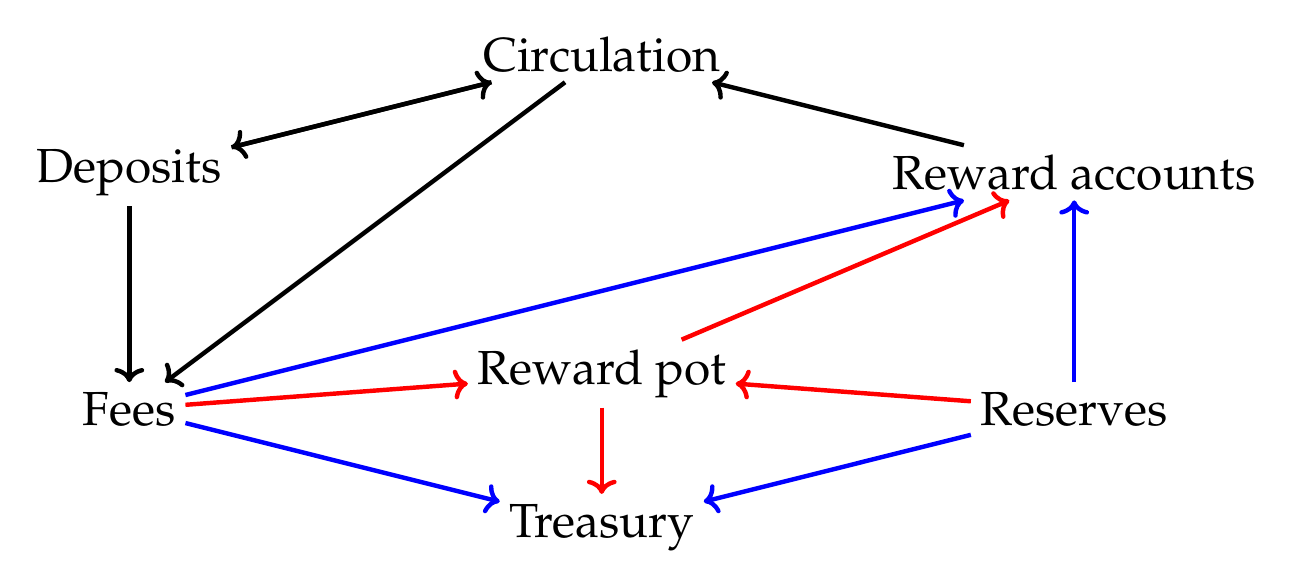
\begin{tikzpicture}
      [ x=30mm, y=30mm
      , direct/.style={black, draw}
      , implied/.style={blue, draw}
      , toTotPot/.style={red, draw}
      ]
    \node (C) at (3,2.5) {\LARGE Circulation};
    \node (R) at (5, 1) {\LARGE Reserves};
    \node (D) at (1, 2) {\LARGE Deposits};
    \node (FR) at (1,1) {\LARGE Fees};
    \node (RA) at (5, 2) {\LARGE Reward accounts};
    \node (T) at (3,0.5) {\LARGE Treasury};

    \draw[->, direct, ultra thick]
    (C) edge (D)
    (C) edge (FR)

    (D) edge (C)
    (D) edge (FR)

    (RA) edge (C);

    \draw[->, implied, ultra thick]
    (FR) edge (T)
    (FR) edge (RA)

    (R) edge (T)
    (R) edge (RA);

    \node (TP) at (3, 1.15) {\LARGE Reward pot};

    \draw[->, toTotPot, ultra thick]
    (FR) edge (TP)
    (R) edge (TP)

    (TP) edge (RA)
    (TP) edge (T);
    \end{tikzpicture}
  \end{center}
  \caption{Preservation of Value}
  \label{fig:fund-preservation}
\end{figure}

Figure~\ref{fig:defs:reward-update} defines a reward update.
It consists of four pots:
\begin{itemize}
  \item The change to the treasury. This will be a positive value.
  \item The change to the reserves. This will be a negative value.
  \item The map of new individual rewards (to be added to the existing rewards).
  \item The change to the fee pot. This will be a negative value.
    rewards.
\end{itemize}

%%
%% Figure - Reward Update Defs
%%
\begin{figure}[htb]
  \emph{Reward Update}
  \begin{equation*}
    \RewardUpdate =
    \left(
      \begin{array}{r@{~\in~}ll}
        \Delta t & \Coin & \text{change to the treasury} \\
        \Delta r & \Coin & \text{change to the reserves} \\
        \var{rs} & \AddrRWD\mapsto\Coin & \text{new individual rewards} \\
        \Delta f & \Coin & \text{change to the fee pot} \\
      \end{array}
    \right)
  \end{equation*}
  %
  \caption{Rewards Update type}
  \label{fig:defs:reward-update}
\end{figure}

\clearpage

Figure~\ref{fig:functions:reward-update-creation} defines two functions,
$\fun{createRUpd}$ to create a reward update and $\fun{applyRUpd}$ to apply a
reward update to an instance of $\EpochState$.

The $\fun{createRUpd}$ function does the following:
\begin{itemize}
  \item Note that for all the calculations below, we use the previous protocol parameters
    $\var{prevPp}$, which corresponds to the parameters during the epoch for which we
    are creating rewards.
  \item First we calculate the change to the reserves,
    as determined by the $\rho$ protocol parameter.
  \item Next we calculate $\var{rewardPot}$, the total amount of coin available for rewards this
    epoch, as described in section 6.4 of \cite{delegation_design}. It consists of four pots:
    \begin{itemize}
      \item The fee pot, containing the transaction fees from the epoch.
      \item The amount of coin in the deposit pot that is no longer needed, due to decay.
      \item The amount of monetary expansion from the reserves, calculated above.
    \end{itemize}
    Note that the fee pot and the decayed amount are taken from the snapshot taken at the
    epoch boundary.  (See~Figure\ref{fig:rules:snapshot}).
  \item Next we calculate the proportion of the reward pot that will move to the treasury,
    as determined by the $\tau$ protocol parameter. The remaining pot is called the
    $\var{R}$, just as in section 6.5 of \cite{delegation_design}.
  \item The rewards are calculated, using the oldest stake distribution snapshot (the one
    labeled ``go'').
    As given by $\fun{maxPool}$, each pool can receive a maximal amount, determined by its
    performance.  The difference between the maximal amount and the actual amount received is
    added to the amount moved to the treasury.
  \item The fee pot will be reduced by $\var{feeSS}$.
\end{itemize}

Note that fees are not explicitly removed from any account:
the fees come from transactions paying them and are accounted for whenever
transactions are processed and when the deposit decay value comes from returning
smaller refunds for deposits than were paid upon depositing.

The $\fun{applyRUpd}$ function does the following:
    \begin{itemize}
      \item Adjust the treasury, reserves and fee pots by the appropriate amounts.
      \item Add each individual reward to the global reward mapping.
    \end{itemize}

These two functions will be used in the blockchain transition systems in Section~\ref{sec:chain}.
In particular,
$\fun{createRUpd}$ will be used in Equation~\ref{eq:reward-update},
and $\fun{applyRUpd}$ will be used in Equation~\ref{eq:new-epoch}.

%%
%% Figure - The Reward Update Creation
%%
\begin{figure}[htb]
  \emph{Calculation to create a reward update}
  %
  \begin{align*}
    & \fun{createRUpd} \in \BlocksMade \to \EpochState \to \Coin \to \RewardUpdate \\
    & \createRUpd{b}{es}{total} = \left(
      \Delta t_1+\Delta t_2,-~\Delta r,~\var{rs},~-\var{feeSS}\right) \\
    & ~~~\where \\
    & ~~~~~~~(\var{acnt},~\var{ss},~\var{ls},~\var{prevPp},~\wcard) = \var{es} \\
    & ~~~~~~~(\wcard,~\wcard,~\var{pstake_{go}},~\var{poolsSS},~\var{feeSS}) = \var{ss}\\
    & ~~~~~~~(\var{stake},~\var{delegs}) = \var{pstate_{go}} \\
    & ~~~~~~~(\wcard,~\var{reserves}) = \var{acnt} \\
    & ~~~~~~~\left(
      \wcard,~
      \left(
      \left(\wcard,~\var{rewards},~\wcard,~\wcard,~\wcard,~\wcard\right)~
      \wcard
      \right)
      \right) = \var{ls} \\
    & ~~~~~~~\Delta r = \floor*{\min(1,\eta) \cdot (\fun{rho}~\var{prevPp}) \cdot
      \var{reserves}}
    \\
    & ~~~~~~~\eta = \frac{blocksMade}{\SlotsPerEpoch \cdot \ActiveSlotCoeff} \\
    & ~~~~~~~\var{rewardPot} = \var{feeSS} + \Delta r \\
    & ~~~~~~~\Delta t_1 = \floor*{(\fun{tau}~\var{prevPp}) \cdot \var{rewardPot}} \\
    & ~~~~~~~\var{R} = \var{rewardPot} - \Delta t_1 \\
    & ~~~~~~~\var{circulation} = \var{total} - \var{reserves} \\
    & ~~~~~~~\var{rs}
      = \reward{prevPp}{b}{R}{(\dom{rewards})}{poolsSS}{stake}{delegs}{circulation} \\
    & ~~~~~~~\Delta t_{2} = R - \left(\sum\limits_{\_\mapsto c\in\var{rs}}c\right) \\
    & ~~~~~~~blocksMade = \sum_{\wcard \mapsto m \in b}m
  \end{align*}

  \caption{Reward Update Creation}
  \label{fig:functions:reward-update-creation}
\end{figure}

\begin{figure}[htb]
  \emph{Applying a reward update}
  %
  \begin{align*}
      & \fun{applyRUpd} \in \RewardUpdate \to \EpochState \to \EpochState \\
      & \fun{applyRUpd}~
      \left(
        \begin{array}{c}
          \Delta t \\
          \Delta r \\
          \var{rs} \\
          \Delta f \\
        \end{array}
    \right)
      \left(
        \begin{array}{c}
          \var{treasury} \\
          \var{reserves} \\
          ~ \\
          \var{stkCreds} \\
          \var{rewards} \\
          \var{delegations} \\
          \var{ptrs} \\
          \var{genDelegs} \\
          \var{i_{rwd}}
          \\~ \\
          \var{stpools} \\
          \var{poolParams} \\
          \var{retiring} \\
          ~ \\
          \var{utxo} \\
          \var{deposits} \\
          \var{fees} \\
          \var{up} \\
          ~ \\
          \var{prevPp} \\
          \var{pp} \\
        \end{array}
      \right)
      =
      \left(
        \begin{array}{c}
          \varUpdate{\var{treasury} + \Delta t}\\
          \varUpdate{\var{reserves} + \Delta r}\\
          ~ \\
          \var{\var{stkCreds}} \\
          \varUpdate{\var{rewards}\unionoverridePlus\var{rs}} \\
          \var{delegations} \\
          \var{ptrs} \\
          \var{genDelegs} \\
          \var{i_{rwd}}
          \\~ \\
          \var{stpools} \\
          \var{poolParams} \\
          \var{retiring} \\
          ~ \\
          \var{utxo} \\
          \var{deposits} \\
          \varUpdate{\var{fees}+\Delta f} \\
          \var{up} \\
          ~ \\
          \var{prevPp} \\
          \var{pp} \\
        \end{array}
    \right)
  \end{align*}

  \caption{Reward Update Application}
  \label{fig:functions:reward-update-application}
\end{figure}

\clearpage

\section{Formal Properties}
\label{sec:properties}

This appendix collects the main formal properties that the new ledger rules are expected to satisfy.

\begin{enumerate}[label=P{\arabic*}:\ ]
\item
  \emph{Consistency with Shelley.}
  All formal properties that were defined for Shelley in \ref{XX} remain valid.\todo{Confirm this, or list any exceptions.}
\item
  \emph{Consistency with Multi-Asset.}
  All formal properties that were defined for multi-asset tokens in \ref{XX} also remain valid.\todo{Confirm this, or list any exceptions.}
\item
  \emph{Ada Consistency.}
  Any token with the $\PolicyID$ of Ada is an Ada token, i.e. it
  also has the $\AssetID$ of Ada.
\item
  \emph{General Accounting.}
  The \emph{general accounting} property\todo{Reference or explain this} holds for any transaction,
  whether it is fully processed or just paying fees. In particular,
  this implies that the total amount of Ada in the system is constant.
\item
  \emph{Fee Movement.}
  If a transaction is accepted and marked as paying fees only
  (i.e. $\fun{txvaltag}\, tx = \True$), then the only change to the ledger
  when processing the transaction is that the inputs marked for paying
  fees are moved to the fee pot.
\item
  \emph{Transaction Validation.}
  If a Shelley transaction is accepted, it is fully processed.\todo{What does this mean? Is this: Transaction consistency - any transaction that is successfully validated can be executed successfully by the interpreter.}
\item
  \emph{Extended UTxO Validation.}
  If a transaction extends the UTxO, all its scripts validate, and
  if it has a script that does not validate, it cannot extend the
  UTxO.
\item
  \emph{Non-Token Forging.}
  A valid transaction that does not forge tokens satisfies the
  accounting property of the Shelley ledger where the type $\Coin$ is
  replaced by $\Value$.
\item
  \todo{\emph{Script consistency.} Scripts are only processed by valid version of the interpreter.}
\item
  \todo{\emph{Backwards compatibility.} All scripts that could be processed by any previous version of the interpreter
    remain valid indefinitely.}
\item
  \todo{\emph{Cost consistency.} - no transaction exceeds the specified resource bounds.}
\item
  \todo{\emph{Backwards Compatibility.} Any transaction that was accepted in a previous version of the ledger rules
    has exactly the same cost and effect, except that the transaction output is extended.}
\item
  ... \todo{Anything else?}
\end{enumerate}

In the ledger there are several cases where non-integral calculations are
required. This does concern the delegation transitions, not value transactions.

\subsection{Types of Non-Integral Calculations}
\label{sec:types-non-integral}

The specification employs non-integral calculations for different mathematical
operations. Table~\ref{tab:func-non-integral} shows the function and transition
rules that use non-integral calculations and which type.

\begin{table}[ht]
  \centering
  \begin{tabular}{lccccc}
    \toprule
    name & page & multiplication & division & exponential function & exponentiation \\
    \midrule
    \fun{refund}
         & \pageref{fig:functions:deposits-refunds} & \checkmark & & \checkmark & \\
    \fun{maxPool}
         & \pageref{fig:functions:rewards} & \checkmark & \checkmark & & \\
    \fun{movingAvg}
         & \pageref{fig:functions:rewards} & \checkmark & \checkmark && \\
    \fun{poolReward}
         & \pageref{fig:functions:rewards} & \checkmark & & \checkmark &
                                                                         \checkmark \\
    \fun{r_{leader}}
         & \pageref{fig:functions:reward-splitting} & \checkmark & \checkmark &&\\
    \fun{mReward}
         & \pageref{fig:functions:reward-splitting} & \checkmark & \checkmark
                                            &&\\
    \fun{rewardOnePool}
         & \pageref{fig:functions:reward-calc} & \checkmark & \checkmark && \\
    \fun{updateAvgs}
         & \pageref{fig:functions:epoch} & \checkmark & \checkmark &&\\
    \fun{ACCNT}
         &\pageref{fig:rules:accnt} & \checkmark &&& \\
    \bottomrule
  \end{tabular}
  \caption{Functions with Non-Integral Calculation}
  \label{tab:func-non-integral}
\end{table}

The transcendental exponential function is used in reward and refund calculation
to model the decay of the deposit values. The pool reward uses exponentiation to
calculate a pool's ranking.

The domain for the exponential function are the non-negative reals, more
precisely the distribution parameter $\lambda \in (0, \infty)$ multiplied by a
discrete non-negative duration $\delta$.

The domain of the base of the exponentiation in $\fun{poolReward}$ are the
non-negative reals resulting from the calculation in $\fun{movingAvg}$, the
exponent $\gamma$ is a constant take from the protocol parameters.

\subsection{Implementation of Non-Integer Calculations}
\label{sec:impl-non-integ}

The large part consists of multiplication and division which can easily be done
using fractional arithmetic to the desired precision. The precision necessary is
bounded by the ability to represent a single lovelace in all calculations.

\subsubsection{Function Simplification}
\label{sec:funct-simpl}

The transcendental function $e^{x}$ can be approximated using different
approaches, depending on the desired accuracy. In general, one uses the
exponential laws $e^{x} = 1/e^{-x}$ and
$e^{x} = \left(e^{\frac{x}{n}} \right)^{n}, n \in \mathbb{N}$ to reduce the
approximation to the unit interval and apply fast integral exponentiation
afterwards.

Exponentiation is implemented using the law
$a^{b} = e^{\ln(a^{b})}= e^{b\ln(a)}$. This therefore requires being able to
calculate $e^{x}$ and $\ln(x)$. The approximation of the natural logarithm can
be approximated using different approaches, again, depending on the desired
accuracy. Most approximations work for $\ln(x), x \in [1, c)$ with some $c >
0$. One then uses the law $\log_{b}(x) = \log_{b}(\frac{x}{b^{n}}b^{n})$ where
$n \in \mathbb{N}$ is chosen in such a way that $\frac{x}{b^{n}} \in [1,
c)$. Using this, one can separate the calculation of the integral and decimal
part as follows:

\begin{equation*}
  \log_{b}(\frac{x}{b^{n}}b^{n})=\log_{b}(b^{n}) + \log_{b}(\frac{x}{b^{n}})=
  n + \log(\frac{x}{b^{n}})
\end{equation*}

%%% Local Variables:
%%% mode: latex
%%% TeX-master: "ledger-spec"
%%% End:


\newpage


%%
%% Byron Spec
%%

\newcommand{\leteq}{\ensuremath{\mathrel{\mathop:}=}}
\newcommand{\SkVk}{\type{SkVk}}
\newcommand{\hash}[1]{\fun{hash}~ \var{#1}}
\newcommand{\Lovelace}{\type{Lovelace}}
\newcommand{\balance}[1]{\fun{balance}~ \var{#1}}
\newcommand{\addr}[1]{\fun{addr}~ \var{#1}}
\newcommand{\wits}[1]{\fun{wits}~ \var{#1}}
\newcommand{\SlotCount}{\type{SlotCount}}
\newcommand{\DSEnv}{\type{DSEnv}}
\newcommand{\DSState}{\type{DSState}}
\newcommand\Set[2]{\{\,#1\mid#2\,\}}
\newcommand{\Bool}{\type{Bool}}
\newcommand{\txs}{\ensuremath{\mathcal{T}}}
\newcommand{\transtar}[2]{\xlongrightarrow[\textsc{#1}]{#2}\negthickspace^{*}}

\section{Introduction}
\label{sec:introduction}

This specification models the \textit{conditions} that the different parts of a
transaction have to fulfill so that they can extend a ledger, which is
represented here as a list of transactions. In particular, we model the
following aspects:

\begin{description}
\item[Preservation of value] relationship between the total value of input and
  outputs in a new transaction, and the unspent outputs.
\item[Witnesses] authentication of parts of the transaction data by means of
  cryptographic entities (such as signatures and private keys) contained in
  these transactions.
\item[Delegation] validity of delegation certificates, which delegate
  block-signing rights.
\item[Update validation] voting mechanism which captures the identification of
  the voters, and the participants that can post update proposals.
\end{description}

The following aspects will not be modeled (since they are not part of the Byron
release):
\begin{description}
\item[Stake] staking rights associated to an addresses.
\end{description}

\newcommand{\pto}{\to_{*}}

\section{Notation}

This specification features some changes to the notation used in previous specifications.

\begin{description}
\item[Maps and partial functions] We use the notation $f : A \pto B$
  to denote a finitely supported partial function. If $B$ is a monoid,
  $f$ is a function such that $f a = 0$ for all but finitely many
  $a$. Otherwise it is a function $f : A \to B^?$ such that
  $f a = \Nothing$ for all but finitely many $a$.
\item[Map operations] We use standard notation for restriction and
  corestriction of functions to operate on partial functions as well.
\end{description}


\section{Cryptographic primitives}
\label{sec:crypto-primitives}

Figure~\ref{fig:crypto-defs} introduces the cryptographic abstractions used in
this document.

\begin{figure}[htb]
  \emph{Abstract types}
  %
  \begin{equation*}
    \begin{array}{r@{~\in~}lr}
      \var{vk} & \SKey & \text{signing key}\\
      \var{vk} & \VKey & \text{verifying key}\\
      \var{hk} & \Hash & \text{hash of a key}\\
      \sigma & \Sig  & \text{signature}\\
      \var{d} & \Data  & \text{data}\\
    \end{array}
  \end{equation*}
  \emph{Derived types}
  \begin{equation*}
    \begin{array}{r@{~\in~}lr}
      (sk, vk) & \SkVk & \text{signing-verifying key pairs}
    \end{array}
  \end{equation*}
  \emph{Abstract functions}
  %
  \begin{equation*}
    \begin{array}{r@{~\in~}lr}
      \hash{} & \VKey \to \Hash
      & \text{hash function} \\
      %
      \fun{verify} & \VKey \times \Data \times \Sig
      & \text{verification relation}\\
    \end{array}
  \end{equation*}
  \emph{Constraints}
  \begin{align*}
    & \forall (sk, vk) \in \SkVk,~ m \in \Data,~ \sigma \in \Sig \cdot
      \verify{vk}{m}{\sigma} \iff \sign{sk}{m} = \sigma
  \end{align*}
  \emph{Notation for serialized and verified data}
  \begin{align*}
    & \serialised{x} & \text{serialised representation of } x\\
    & \mathcal{V}_{\var{vk}}{\serialised{m}}_{\sigma} = \verify{vk}{m}{\sigma}
      & \text{shorthand notation for } \fun{verify}
  \end{align*}
  \caption{Cryptographic definitions}
  \label{fig:crypto-defs}
\end{figure}
\newcommand{\PPMMap}{\ensuremath{\type{PParams}}}
\newcommand{\Lmax}{\ensuremath{\mathbb{L}_{\var{max}}}}
\section{UTxO}
\label{sec:state-trans-utxo-1}

The transition rules for unspent outputs are presented in
Figure~\ref{fig:rules:utxo}. The states of the UTxO transition system, along
with their types are defined in Figure~\ref{fig:defs:utxo}, here we define the
protocol parameters as an abstract type, this type is made concrete in
Section~\ref{sec:update}, where the update mechanism is discussed. Functions on
these types are defined in Figure~\ref{fig:derived-defs:utxo}. In particular,
note that in function $\fun{minfee}$ we make use of the fact that the
$\Lovelace$ type is an alias for the set of the integers numbers
($\mathbb{Z}$).

\begin{figure*}[htb]
  \emph{Abstract types}
  %
  \begin{equation*}
    \begin{array}{r@{~\in~}lr}
      \var{tx} & \Tx & \text{transaction}\\
      %
      \var{txid} & \TxId & \text{transaction id}\\
      %
      ix & \Ix & \text{transaction index}\\
      %
      \var{addr} & \Addr & \text{address}\\
      %
      \var{pps} & \PPMMap & \text{protocol parameters}
    \end{array}
  \end{equation*}
  %
  \emph{Derived types}
  %
  \begin{equation*}
    \begin{array}{r@{~\in~}l@{\qquad=\qquad}r@{~\in~}lr}
      \ell & \Lovelace
      & n  & \mathbb{Z}
      & \text{currency value}
      \\
      \var{txin}
      & \TxIn
      & (\var{txid}, \var{ix})
      & \TxId \times \Ix
      & \text{transaction input}
      \\
      \var{txout}
      & \type{TxOut}
      & (\var{addr}, c)
      & \Addr \times \Lovelace
      & \text{transaction output}
      \\
      \var{utxo}
      & \UTxO
      & m
      & \TxIn \mapsto \TxOut
      & \text{unspent tx outputs}
    \end{array}
  \end{equation*}
  %
  \emph{Abstract Functions}
  \begin{equation*}
    \begin{array}{r@{~\in~}lr}
      \txid{} & \Tx \to \TxId & \text{compute transaction id}\\
      %
      \fun{txbody} & \Tx \to \powerset{\TxIn} \times (\Ix \mapsto \TxOut)
                                  & \text{transaction body}\\
      %
      \fun{a} & \PPMMap \to \mathbb{Z} & \text{minumum fee factor}\\
      %
      \fun{b} & \PPMMap \to \mathbb{Z} & \text{minumum fee constant}\\
      %
      \fun{txSize} & \Tx \to \mathbb{Z} & \text{abstract size of a transaction}
    \end{array}
  \end{equation*}
  %
  \emph{Constraints}
  \begin{equation}
    \label{eq:txid-injective}
    \forall \var{tx_i}, \var{tx_j} \cdot
    \txid{\var{tx_i}} = \txid{\var{tx_j}} \Rightarrow \var{tx_i} = \var{tx_j}
  \end{equation}
  \caption{Definitions used in the UTxO transition system}
  \label{fig:defs:utxo}
\end{figure*}

\begin{figure}
  \begin{align*}
    & \fun{txins} \in \Tx \to \powerset{\TxIn}
    & \text{transaction inputs} \\
    & \txins{tx} = \var{inputs} \where \txbody{tx} = (\var{inputs}, ~\wcard)
    \nextdef
    & \fun{txouts} \in \Tx \to \UTxO
    & \text{transaction outputs as UTxO} \\
    & \fun{txouts} ~ \var{tx} =
      \left\{ (\fun{txid} ~ \var{tx}, \var{ix}) \mapsto \var{txout} ~
      \middle| \begin{array}{l@{~}c@{~}l}
                 (\_, \var{outputs}) & = & \txbody{tx} \\
                 \var{ix} \mapsto \var{txout} & \in & \var{outputs}
               \end{array}
      \right\}
    \nextdef
    & \fun{balance} \in \UTxO \to \mathbb{Z}
    & \text{UTxO balance} \\
    & \fun{balance} ~ utxo = \sum_{(~\wcard ~ \mapsto (\wcard, ~c)) \in \var{utxo}} c\\
   \nextdef
   %
    & \fun{minfee} \in \PPMMap \to \Tx \to \mathbb{Z} & \text{minimum fee}\\
    & \fun{minfee}~\var{pps}~\var{tx} =
      \fun{a}~\var{pps} * \fun{txSize}~\var{tx} + \fun{b}~\var{pps}
  \end{align*}
  \caption{Functions used in UTxO rules}
  \label{fig:derived-defs:utxo}
\end{figure}

\begin{figure}
  \emph{UTxO environments}
  \begin{equation*}
    \UTxOEnv =
    \left(
      \begin{array}{r@{~\in~}lr}
        \var{utxo_0} & \UTxO & \text{genesis UTxO}\\
        \var{pps} & \PPMMap & \text{protocol parameters map}\\
      \end{array}
    \right)
  \end{equation*}

  \emph{UTxO transitions}
  \begin{equation*}
    \_ \vdash
    \var{\_} \trans{utxo}{\_} \var{\_}
    \subseteq \powerset (\UTxOEnv \times \UTxO \times \Tx \times \UTxO)
  \end{equation*}
  \caption{UTxO transition-system types}
  \label{fig:ts-types:utxo}
\end{figure}

\begin{figure}
  \begin{equation}\label{eq:utxo-bootstrap}
    \inference
    {
    }
    {
      {\begin{array}{l}
        utxo_0\\
        pps
      \end{array}}
      \vdash
      \var{utxo_0}
    }
  \end{equation}
  \nextdef
  \begin{equation}\label{eq:utxo-inductive}
    \inference
    { \txins{tx} \subseteq \dom \var{utxo}
      & \minfee{pps}{tx} \leq \balance{(\txouts{tx})} - \balance{(\txins{tx} \restrictdom \var{utxo})}\\
      \txins{tx} \neq \emptyset
    }
    {
      {\begin{array}{l}
        utxo_0\\
        pps
      \end{array}}
      \vdash
      \var{utxo}
      \trans{utxo}{tx}
      (\txins{tx} \subtractdom \var{utxo}) \cup \txouts{tx}
    }
  \end{equation}
  \caption{UTxO inference rules}
  \label{fig:rules:utxo}
\end{figure}

Rule~\ref{eq:utxo-inductive} specifies under which conditions a transaction can
be applied to a set of unspent outputs, and how the set of unspent output
changes with a transaction:
\begin{itemize}
\item Each input spent in the transaction must be in the set of unspent
  outputs.
\item The minimum fee, which depends on the transaction and the protocol
  parameters, must be less or equal than the difference between the balance of
  the unspent outputs in a transaction (i.e. the total amount paid in a
  transaction) and the amount of spent inputs.
\item The set of inputs must not be empty.
\item If the above conditions hold, then the new state will not have the inputs
  spent in transaction $\var{tx}$ and it will have the new outputs in
  $\var{tx}$.
\end{itemize}

\clearpage

\subsection{Witnesses}
\label{sec:witnesses}

The rules for witnesses are presented in Figure~\ref{fig:rules:utxow}.
The definitions used in Rule~\ref{eq:utxo-witness-inductive} are given in
Figure~\ref{fig:defs:utxow}. Note that
Rule~\ref{eq:utxo-witness-inductive} uses the transition relation defined in
Figure~\ref{fig:rules:utxo}. The main reason for doing this is to define
the rules incrementally, modeling different aspects in isolation to keep the
rules as simple as possible. Also note that the $\trans{utxo}{}$ relation could
have been defined in terms of $\trans{utxow}{}$ (thus composing the rules in a
different order). The choice here is arbitrary.

\begin{figure}[htb]
  \emph{Abstract functions}
  %
  \begin{equation*}
    \begin{array}{r@{~\in~}lr}
      \fun{wits} & \Tx \to \powerset{(\VKey \times \Sig)}
      & \text{witnesses of a transaction}\\
      \fun{hash_{spend}} & \Addr \mapsto \HashKey
      & \text{hash of a spending key in an address}\\
    \end{array}
  \end{equation*}
  \caption{Definitions used in the UTxO transition system with witnesses}
  \label{fig:defs:utxow}
\end{figure}

\begin{figure}[htb]
  \begin{align*}
    & \addr{}{} \in \UTxO \to \TxIn \mapsto \Addr & \text{address of an input}\\
    & \addr{utxo} = \{ i \mapsto a \mid i \mapsto (a, \wcard) \in \var{utxo} \} \\
    \nextdef
    & \fun{addr_h} \in \UTxO \to \TxIn \mapsto \HashKey & \text{hash of an input address}\\
    & \fun{addr_h}~utxo = \{ i \mapsto h \mid i \mapsto (a, \wcard) \in \var{utxo}
      \wedge a \mapsto h \in \fun{hash_{spend}} \}
  \end{align*}
  \caption{Functions used in rules witnesses}
  \label{fig:derived-defs:utxow}
\end{figure}

\begin{figure}
  \emph{UTxO with witness transitions}
  \begin{equation*}
    \var{\_} \vdash
    \var{\_} \trans{utxow}{\_} \var{\_}
    \subseteq \powerset (\PPMMap \times \UTxO \times \Tx \times \UTxO)
  \end{equation*}
  \caption{UTxO with witness transition-system types}
  \label{fig:ts-types:utxow}
\end{figure}

\begin{figure}
  \begin{equation}
    \label{eq:utxo-witness-inductive}
    \inference
    { \var{pps} \vdash \var{utxo} \trans{utxo}{tx} \var{utxo'}
      & \var{maxTxSize} \mapsto \var{t} \in \var{pps} & \fun{txSize}~\var{tx} \leq t \\ ~ \\
      & \forall i \in \txins{tx} \cdot \exists (\var{vk}, \sigma) \in \wits{\var{tx}}
      \cdot
      \mathcal{V}^\sigma_{\var{vk}}~{\serialised{\txbody{tx}}}
      \wedge  \fun{addr_h}~{utxo}~i = \hash{vk}\\
    }
    {\var{pps} \vdash \var{utxo} \trans{utxow}{tx} \var{utxo'}}
  \end{equation}
  \caption{UTxO with witnesses inference rules}
  \label{fig:rules:utxow}
\end{figure}

\section{Delegation}
\label{sec:delegation}

An agent owning a key that can sign new blocks can delegate its signing rights
to another key by means of \textit{delegation certificates}. These certificates
are included in the ledger, and therefore also included in the body of the
blocks in the blockchain.

There are several restrictions on a certificate posted on the blockchain:
\begin{enumerate}
\item Only genesis keys can delegate.
\item Certificates must be properly signed by the delegator.
\item Any given key can delegate at most once per-epoch.
\item Any given key can issue at most one certificate in a given slot.
\item The epochs in the certificates must refer to the current or to the next
  epoch. We do not want to allow certificates from past epochs so that a
  delegation certificate cannot be replayed. On the other hand if we allow
  certificates with arbitrary future epochs, then a malicious key can issue a
  delegation certificate per-slot, setting the epoch to a sufficiently large
  value. This will cause a blow up in the size of the ledger state since we
  will not be able to clean $\var{eks}$ (we only clean past epochs). Also note
  that we do not check the relation between the certificate epoch and the slot
  in which the certificate becomes active. This would bring additional
  complexity without any obvious benefit.
\item Certificates do not become active immediately, but they require a certain
  number of slots till they become stable in all the nodes.
\end{enumerate}
These conditions are formalized in \cref{fig:rules:delegation-scheduling}.
Rule~\ref{eq:rule:delegation-scheduling} determines when a certificate can
become ``scheduled''. The definitions used in this rules are presented in
\cref{fig:defs:delegation-scheduling}, and the types of the system induced by
$\trans{sdeleg}{\wcard}$ are presented in
\cref{fig:ts-types:delegation-scheduling}.

\begin{figure}[htb]
  \emph{Abstract types}
  \begin{equation*}
    \begin{array}{r@{~\in~}lr}
      c & \DCert & \text{delegation certificate}\\
      \var{vk_g} & \VKeyGen & \text{genesis verification key}\\
    \end{array}
  \end{equation*}

  \emph{Derived types}
  \begin{equation*}
    \begin{array}{r@{~\in~}l@{\qquad=\qquad}r@{~\in~}lr}
      \var{e} & \Epoch & n & \mathbb{N} & \text{epoch}\\
      \var{s} & \Slot & s & \mathbb{N} & \text{slot}\\
      \var{d} & \SlotCount & s & \mathbb{N} & \text{slot}
    \end{array}
  \end{equation*}

  \emph{Constraints}
  \begin{align*}
    \VKeyGen \subseteq \VKey
  \end{align*}

  \emph{Abstract functions}
  \begin{equation*}
    \begin{array}{r@{~\in~}lr}
      \fun{dbody} & \DCert \to (\VKey \times \Epoch)
      & \text{body of the delegation certificate}\\
      \fun{dwit} & \DCert \to (\VKeyGen \times \Sig)
      & \text{witness for the delegation certificate}\\
      \fun{dwho} & \DCert \mapsto (\VKeyGen \times \VKey)
      & \text{who delegates to whom in the certificate}\\
      \fun{depoch} & \DCert \mapsto \Epoch
      & \text{certificate epoch}
    \end{array}
  \end{equation*}
  \caption{Delegation scheduling definitions}
  \label{fig:defs:delegation-scheduling}
\end{figure}

\begin{figure}[htb]
  \emph{Delegation scheduling environments}
  \begin{equation*}
    \DSEnv =
    \left(
      \begin{array}{r@{~\in~}lr}
        \mathcal{K} & \powerset{\VKeyGen} & \text{allowed delegators}\\
        \var{e} & \Epoch & \text{epoch}\\
        \var{s} & \Slot & \text{slot}\\
        \var{k} & \SlotCount & \text{chain stability parameter}
      \end{array}
    \right)
  \end{equation*}

  \emph{Delegation scheduling states}
  \begin{equation*}
    \DSState
    = \left(
      \begin{array}{r@{~\in~}lr}
        \var{sds} & \seqof{(\Slot \times (\VKeyGen \times \VKey))} & \text{scheduled delegations}\\
        \var{eks} & \powerset{(\Epoch \times \VKeyGen)} & \text{key-epoch delegations}
      \end{array}
    \right)
  \end{equation*}

  \emph{Delegation scheduling transitions}
  \begin{equation*}
    \var{\_} \vdash
    \var{\_} \trans{sdeleg}{\_} \var{\_}
    \subseteq \powerset (\DSEnv \times \DSState \times \DCert \times \DSState)
  \end{equation*}
  \caption{Delegation scheduling transition-system types}
  \label{fig:ts-types:delegation-scheduling}
\end{figure}

\begin{figure}[htb]
  \begin{equation}
    \inference
    {
    }
    {
      {\begin{array}{l}
       \mathcal{K}\\
        e\\
        s\\
        d
      \end{array}}
      \vdash
      \left(
        \begin{array}{l}
          \epsilon\\
          \emptyset
        \end{array}
      \right)
    }
  \end{equation}
  \nextdef
  \begin{equation}
    \label{eq:rule:delegation-scheduling}
    \inference
    {
      (\var{vk_s},~ \sigma) \leteq \dwit{c}
      & \verify{vk_s}{\serialised{\dbody{c}}}{\sigma} & vk_s \in \mathcal{K}\\ ~ \\
      (\var{vk_s},~ \var{vk_d}) \leteq \dwho{c} & e_d \leteq \depoch{c}
      & (e_d,~ \var{vk_s}) \notin \var{eks} & 0 \leq e_d - e \leq 1 \\ ~ \\
      d \leteq 2 \cdot k & (s + d,~ (\var{vk_s},~ \wcard)) \notin \var{sds}\\
    }
    {
      {\begin{array}{l}
       \mathcal{K}\\
        e\\
        s\\
        k
      \end{array}}
      \vdash
      {
        \left(
          \begin{array}{l}
            \var{sds}\\
            \var{eks}
          \end{array}
        \right)
      }
      \trans{sdeleg}{c}
      {
        \left(
          \begin{array}{l}
            \var{sds}; (s + d,~ (\var{vk_s},~ \var{vk_d}))\\
            \var{eks} \cup \{(e_d,~ \var{vk_s})\}
          \end{array}
        \right)
      }
    }
  \end{equation}
  \caption{Delegation scheduling rules}
  \label{fig:rules:delegation-scheduling}
\end{figure}

\clearpage

The rules in Figure~\ref{fig:rules:delegation} model the activation of
delegation certificates. Once a scheduled certificate becomes active
(see~\cref{sec:delegation-interface-rules}), the delegation map is changed by
it only if:
\begin{itemize}
\item The delegating key ($\var{vk_s}$) did not activate a delegation
  certificate in a slot greater or equal than the certificate slot ($s$). This
  check is performed to avoid having the constraint that the delegation
  certificates have to be activated in slot order.
\item The key being delegated to ($\var{vk_d}$) has not been delegated by
  another key (injectivity constraint).
\end{itemize}
The reason why we check that the delegation map is injective is to avoid a
potential risk (during the OBFT era) in which a malicious node gets control of
a genesis key $\var{vk_m}$ that issued the maximum number of blocks in a given
window. By delegating to another key $\var{vk_d}$, which was already delegated to
by some other key $\var{vk_g}$, the malicious node could prevent $\var{vk_g}$
from issuing blocks. Even though the delegation certificates take several slots
to become effective, the malicious node could calculate when the certificate
would become active, and issue a delegation certificate at the right time.

As an additional advantage, by having an injective delegation map, we are able
to simplify our specification when it comes to counting the blocks issued by
(delegates of) genesis keys.

Note also, that we could not impose the injectivity constraint in
Rule~\ref{eq:rule:delegation-scheduling} since we do not have information about
the delegations that will become effective. We could of course detect a
violation in the injectivity constraint when scheduling a delegation
certificate, but this will lead to a complex computation and larger state in
said rule.

Finally, note that we do not want to reject a scheduled delegation that would
violate the injectivity constraint (since delegation might not have been
scheduled by the node issuing the block). Instead, we simply ignore the
delegation certificate (Rule~\ref{eq:rule:delegation-nop}).

\begin{figure}[htb]
  \begin{align*}
    & \unionoverrideRight \in (A \mapsto B) \to (A \mapsto B) \to (A \mapsto B)
    & \text{union override}\\
    & d_0 \unionoverrideRight d_1 = d_1 \cup (\dom d_1 \subtractdom d_0)
  \end{align*}
  \caption{Functions used in delegation rules}
  \label{fig:funcs:delegation}
\end{figure}

\begin{figure}[htb]
  \emph{Delegation environments}
  \begin{equation*}
    \DEnv =
    \left(
      \begin{array}{r@{~\in~}lr}
        \mathcal{K} & \powerset{\VKeyGen} & \text{allowed delegators}
      \end{array}
    \right)
  \end{equation*}

  \emph{Delegation states}
  \begin{align*}
    & \DState
      = \left(
        \begin{array}{r@{~\in~}lr}
          \var{dms} & \VKeyGen \mapsto \VKey & \text{delegation map}\\
          \var{dws} & \VKeyGen \mapsto \Slot & \text{when last delegation occurred}\\
        \end{array}\right)
  \end{align*}
  \emph{Delegation transitions}
  \begin{equation*}
    \_ \vdash \_ \trans{adeleg}{\_} \_ \in
    \powerset (\DEnv \times \DState \times (\Slot \times (\VKeyGen \times \VKey)) \times \DState)
    \end{equation*}
  \caption{Delegation transition-system types}
  \label{fig:ts-types:delegation}
\end{figure}

\begin{figure}[htb]
  \begin{equation}
    \inference
    {
      \var{dms_0} \leteq \Set{k \mapsto k}{k \in \mathcal{K}} &
      \var{dws_0} \leteq \Set{k \mapsto 0}{k \in \mathcal{K}}
    }
    {
      \mathcal{K}
      \vdash
      \left(
        \begin{array}{l}
          \var{dms_0}\\
          \var{dws_0}
        \end{array}
      \right)
    }
  \end{equation}
  \nextdef
  \begin{equation}\label{eq:rule:delegation-change}
    \inference
    {
      \var{vk_d} \notin \range~\var{dms} & (\var{vk_s} \mapsto s_p \in \var{dws} \Rightarrow s_p < s)
    }
    {
      \mathcal{K}
      \vdash
      \left(
      \begin{array}{r}
        \var{dms}\\
        \var{dws}
      \end{array}
      \right)
      \trans{adeleg}{(s,~ (vk_s,~ vk_d))}
      \left(
      \begin{array}{lcl}
        \var{dms} & \unionoverrideRight & \{\var{vk_s} \mapsto \var{vk_d}\}\\
        \var{dws} & \unionoverrideRight & \{\var{vk_s} \mapsto s \}
      \end{array}
      \right)
    }
  \end{equation}
  \nextdef
  \begin{equation}\label{eq:rule:delegation-nop}
    \inference
    {\var{vk_d} \in \range~\var{dms} \vee (\var{vk_s} \mapsto s_p  \in \var{dws}  \wedge s \leq s_p)
    }
    {
      \mathcal{K}
      \vdash
      \left(
      \begin{array}{r}
        \var{dms}\\
        \var{dws}
      \end{array}
      \right)
      \trans{adeleg}{(s,~ (\var{vk_s},~ \var{vk_d}))}
      \left(
      \begin{array}{lcl}
        \var{dms}\\
        \var{dws}
      \end{array}
      \right)
    }
  \end{equation}
  \caption{Delegation inference rules}
  \label{fig:rules:delegation}
\end{figure}

\clearpage

\subsection{Delegation sequences}
\label{sec:delegation-sequences}

This section presents the rules that model the effect that sequences of
delegations have on the ledger.

\begin{figure}[htb]
  \begin{equation}
    \inference[Initial-SDELEGS]
    {
    }
    {
      {\begin{array}{l}
       \mathcal{K}\\
        e\\
        s\\
        d
      \end{array}}
      \vdash
      \left(
        \begin{array}{l}
          \epsilon\\
          \emptyset
        \end{array}
      \right)
    }
  \end{equation}
  \nextdef
  \begin{equation}
    \label{eq:rule:delegation-scheduling-seq-base}
    \inference
    {
    }
    {
      {\begin{array}{l}
         \mathcal{K} \\
         e\\
         s\\
         d
       \end{array}}
      \vdash
      {
        \left(
          \begin{array}{l}
            \var{sds}\\
            \var{eks}
          \end{array}
        \right)
      }
      \trans{sdelegs}{\epsilon}
      {
        \left(
          \begin{array}{l}
            \var{sds}\\
            \var{eks}
          \end{array}
        \right)
      }
    }
  \end{equation}
  \nextdef
  \begin{equation}
    \label{eq:rule:delegation-scheduling-seq-ind}
    \inference
    {
      {\begin{array}{l}
         \mathcal{K} \\
         e\\
         s\\
         d
       \end{array}}
      \vdash
      {
        \left(
          \begin{array}{l}
            \var{sds}\\
            \var{eks}
          \end{array}
        \right)
      }
      \trans{sdelegs}{\Gamma}
      {
        \left(
          \begin{array}{l}
            \var{sds'}\\
            \var{eks'}
          \end{array}
        \right)
      }
      &
      {\begin{array}{l}
         \mathcal{K} \\
         e\\
         s\\
         d
       \end{array}}
      \vdash
      {
        \left(
          \begin{array}{l}
            \var{sds'}\\
            \var{eks'}
          \end{array}
        \right)
      }
      \trans{sdeleg}{c}
      {
        \left(
          \begin{array}{l}
            \var{sds''}\\
            \var{eks''}
          \end{array}
        \right)
      }
    }
    {
      {\begin{array}{l}
         \mathcal{K} \\
         e\\
         s\\
         d
       \end{array}}
      \vdash
      {
        \left(
          \begin{array}{l}
            \var{sds}\\
            \var{eks}
          \end{array}
        \right)
      }
      \trans{sdelegs}{\Gamma; c}
      {
        \left(
          \begin{array}{l}
            \var{sds''}\\
            \var{eks''}
          \end{array}
        \right)
      }
    }
  \end{equation}
  \caption{Delegation scheduling sequence rules}
  \label{fig:rules:delegation-scheduling-seq}
\end{figure}

\begin{figure}
  \begin{equation}
    \inference[Initial-ADELEGS]
    {
      \var{dms_0} \leteq \Set{k \mapsto k}{k \in \mathcal{K}} &
      \var{dws_0} \leteq \Set{k \mapsto 0}{k \in \mathcal{K}}
    }
    {
      \mathcal{K}
      \vdash
      \left(
        \begin{array}{l}
          \var{dms_0}\\
          \var{dws_0}
        \end{array}
      \right)
    }
  \end{equation}
  \nextdef
  \begin{equation}
    \label{eq:rule:delegation-seq-base}
    \inference
    {
    }
    {
      \mathcal{K}
      \vdash
      {
        \left(
          \begin{array}{l}
            \var{dms}\\
            \var{dws}
          \end{array}
        \right)
      }
      \trans{adelegs}{\epsilon}
      {
        \left(
          \begin{array}{l}
            \var{dms}\\
            \var{dws}
          \end{array}
        \right)
      }
    }
  \end{equation}
  \nextdef
  \begin{equation}
    \label{eq:rule:delegation-seq-ind}
    \inference
    {
      {
        \left(
          \begin{array}{l}
            \var{dms}\\
            \var{dws}
          \end{array}
        \right)
      }
      \trans{adelegs}{\Gamma}
      {
        \left(
          \begin{array}{l}
            \var{dms'}\\
            \var{dws'}
          \end{array}
        \right)
      }
      &
      {
        \left(
          \begin{array}{l}
            \var{dms'}\\
            \var{dws'}
          \end{array}
        \right)
      }
      \trans{adeleg}{c}
      {
        \left(
          \begin{array}{l}
            \var{dms''}\\
            \var{dws''}
          \end{array}
        \right)
      }
    }
    {
      \mathcal{K}
      \vdash
      {
        \left(
          \begin{array}{l}
            \var{dms}\\
            \var{dws}
          \end{array}
        \right)
      }
      \trans{adelegs}{\Gamma; c}
      {
        \left(
          \begin{array}{l}
            \var{dms''}\\
            \var{dws''}
          \end{array}
        \right)
      }
    }
  \end{equation}
  \caption{Delegations sequence rules }
  \label{fig:rules:delegation-seq}
\end{figure}

\newcommand{\UProp}{\ensuremath{\type{UProp}}}
\newcommand{\UPropId}{\ensuremath{\type{UpId}}}
\newcommand{\UPropSD}{\ensuremath{\type{UpSD}}}
\newcommand{\ProtVer}{\ensuremath{\type{ProtVer}}}
\newcommand{\ProtPm}{\ensuremath{\type{Ppm}}}
\newcommand{\Rpus}{\ensuremath{\type{Rpus}}}
\newcommand{\UPVEnv}{\ensuremath{\type{UPVEnv}}}
\newcommand{\UPVState}{\ensuremath{\type{UPVState}}}
\newcommand{\UPLEnv}{\ensuremath{\type{UPLEnv}}}
\newcommand{\UPLState}{\ensuremath{\type{UPLState}}}
\newcommand{\UPREnv}{\ensuremath{\type{UPREnv}}}
\newcommand{\UPRState}{\ensuremath{\type{UPRState}}}
\newcommand{\Vote}{\ensuremath{\type{Vote}}}
\newcommand{\VREnv}{\ensuremath{\type{VREnv}}}
\newcommand{\VRState}{\ensuremath{\type{VRState}}}
\newcommand{\VEnv}{\ensuremath{\type{VEnv}}}
\newcommand{\VState}{\ensuremath{\type{VState}}}
\newcommand{\BVREnv}{\ensuremath{\type{BVREnv}}}
\newcommand{\BVRState}{\ensuremath{\type{BVRState}}}
\newcommand{\ApName}{\ensuremath{\type{ApName}}}
\newcommand{\SWVer}{\ensuremath{\type{SWVer}}}
\newcommand{\ApVer}{\ensuremath{\type{ApVer}}}

\newcommand{\upSize}[1]{\ensuremath{\fun{upSize}~\var{#1}}}
\newcommand{\upPV}[1]{\ensuremath{\fun{upPV}~\var{#1}}}
\newcommand{\upId}[1]{\ensuremath{\fun{upId}~\var{#1}}}
\newcommand{\upSig}[1]{\ensuremath{\fun{upSig}~\var{#1}}}
\newcommand{\upSigData}[1]{\ensuremath{\fun{upSigData}~\var{#1}}}
\newcommand{\upIssuer}[1]{\ensuremath{\fun{upIssuer}~\var{#1}}}
\newcommand{\upParams}[1]{\ensuremath{\fun{upParams}~\var{#1}}}
\newcommand{\upSwVer}[1]{\ensuremath{\fun{upSwVer}~\var{#1}}}
\newcommand{\vCaster}[1]{\ensuremath{\fun{vCaster}~\var{#1}}}
\newcommand{\vPropId}[1]{\ensuremath{\fun{vPropId}~\var{#1}}}
\newcommand{\vSig}[1]{\ensuremath{\fun{vSig}~\var{#1}}}

\lstset{ frame=tb,
       , language=Haskell
       , basicstyle=\footnotesize\ttfamily,
       , keywordstyle=\color{blue!80},
       , commentstyle=\itshape\color{purple!40!black},
       , identifierstyle=\bfseries\color{green!40!black},
       , stringstyle=\color{orange},
       }

\lstMakeShortInline[columns=fixed]`

\section{Update mechanism}
\label{sec:update}

This section formalizes the update mechanism by which the protocol parameters
get updated. This formalization is a simplification of the current update
mechanism implemented in
\href{https://github.com/input-output-hk/cardano-sl/}{\texttt{cardano-sl}}, and
partially documented in:
\begin{itemize}
\item \href{https://cardanodocs.com/technical/updater/}{Updater implementation}
\item \href{https://cardanodocs.com/cardano/update-mechanism/}{Update mechanism}
\item
  \href{https://github.com/input-output-hk/cardano-sl/blob/2a19d8ce2941b8e60f0208a5198943ec2ada1fd4/docs/block-processing/us.md}{Update system consensus rules}
\end{itemize}

The reason for formalizing a simplified version of the current implementation
is that research work on blockchain update mechanisms is needed before
introducing a more complex update logic. Since this specification is to be
implemented in a federated setting, some of the constraints put in place in the
current implementation are no longer relevant. Once the research work is ready,
this specification can be extended to incorporate the research results.

\subsection{Update proposals}
\label{sec:update-proposals}

\begin{figure}[htb]
  \emph{Abstract types}
  %
  \begin{equation*}
    \begin{array}{r@{~\in~}lr}
      \var{up} & \UProp & \text{update proposal}\\
      \var{p} & \ProtPm & \text{protocol parameter}\\
      \var{upd} & \type{UpdData} & \text{update data}\\
      \var{upa} & \type{UpdAttrs} & \text{update attributes}\\
      \var{an} & \ApName & \text{application name}
    \end{array}
  \end{equation*}
  %
  \emph{Derived types}
  \begin{equation*}
    \begin{array}{r@{~\in~}l@{~=~}r@{~\in~}lr}
      \var{s_n} & \Slot & n & \mathbb{N} & \text{slot number}\\
      \var{pv} & \ProtVer & (\var{maj}, \var{min}, \var{alt})
      & (\mathbb{N}, \mathbb{N}, \mathbb{N}) & \text{protocol version}\\
      \var{pps} & \PPMMap & \var{pps} & \ProtPm \mapsto \Value
                                         & \text{protocol parameters map}\\
      \var{apv} & \ApVer & n & \mathbb{N}\\
      \var{swv} & \SWVer
      & (\var{an}, \var{av}) & \ApName \times \ApVer
      & \text{software version}\\
      \var{pb} & \UPropSD
      &
        {\left(\begin{array}{r l}
                 \var{pv}\\
                 \var{pps}\\
                 \var{swv}\\
                 \var{upd}\\
                 \var{upa}\\
               \end{array}\right)}
      & {
        \left(
        \begin{array}{l}
          \ProtVer\\
          \PPMMap\\
          \type{SWVer}\\
          \type{UpdData}\\
          \type{UpdAttrs}\\
        \end{array}
                   \right)
                   }
               & \text{protocol update signed data}
    \end{array}
  \end{equation*}
  \emph{Abstract functions}
  %
  \begin{equation*}
    \begin{array}{r@{~\in~}lr}
      \fun{upIssuer} & \UProp \to \VKey & \text{update proposal issuer (delegate)}\\
      \fun{upSize} & \UProp \to \mathbb{N} & \text{update proposal size}\\
      \fun{upPV} & \UProp \to \ProtVer & \text{update proposal protocol version}\\
      \fun{upId} & \UProp \to \UPropId & \text{update proposal id}\\
      \fun{upParams} & \UProp \to \mathbb{\PPMMap}
                                           & \text{proposed parameters update}\\
      \fun{upSwVer} & \UProp \to \SWVer & \text{software-version update proposal}\\
      \fun{upSig} & \UProp \to \Sig & \text{update proposal signature}\\
      \fun{upSigdata} & \UProp \to \UPropSD & \text{update proposal signed data}\\
    \end{array}
  \end{equation*}
  \caption{Update proposals definitions}
  \label{fig:defs:update-proposals}
\end{figure}

The set of protocol parameters ($\ProtPm$) is assumed to contain the following
keys, some of which correspond with fields of the
\href{https://github.com/input-output-hk/cardano-sl/}{\texttt{cardano-sl}}
`BlockVersionData` structure:
\begin{itemize}
\item Slot duration: $\var{slotDuration}$
\item Maximum block size: $\var{maxBlockSize}$
\item Maximum transaction size: $\var{maxTxSize}$
\item Maximum header size: $\var{maxHeaderSize}$
\item Maximum transaction size: $\var{maxTxSize}$
\item Maximum proposal size: $\var{maxProposalSize}$
\item Transaction fee policy: $\var{txFeePolicy}$
\item Script version: $\var{scriptVersion}$
\item Update adoption threshold : $\var{upAdptThd}$. This represents the
  minimum percentage of the total number of genesis keys that have to endorse a
  protocol version to be able to become adopted. This parameter would
  correspond with `srMinThd` in `bvdSoftforkRule`.
\item Chain stability parameter: $\var{stableAfter}$.
\item Update proposal time-to-live: $\var{upropTTL}$. This would correspond to
  the number of slots specified by `bvdUpdateImplicit`. In `cardano-sl` the
  rule was that after `bvdUpdateImplicit` slots, if a proposal did not reach a
  majority of the votes, then if the proposal has more votes for than against
  it, then it will become implicitly accepted, or rejected otherwise. In this
  specification, we re-interpret the meaning of this parameter as the proposal
  time-to-live: if after the number of slots specified by `bvdUpdateImplicit`
  the proposal does not reach a majority of approvals, the proposal is simply
  discarded. In the mainnet configuration (`mainnet-genesis.json` this value is
  set to $10000$, which corresponds with almost half of the total number of
  slots in an epoch).
\end{itemize}
In addition we make use of the $\var{cfmThd}$ key, which determines the portion
of the stakeholders that have to vote for a proposal to consider it confirmed.
This key does not seem to have a corresponding field in `BlockVersionData`, so
to be consistent with the existing chain the value corresponding to
$\var{cfmThd}$ can be set to $4$, which represents the majority of the $7$
genesis keys.

\subsection{Update proposals registration}
\label{sec:update-proposals-registration}

\begin{figure}[htb]
  \emph{Update proposals validity environments}
  \begin{equation*}
    \UPVEnv =
    \left(
      \begin{array}{r@{~\in~}lr}
        \var{pv} & \ProtVer & \text{adopted (current) protocol version}\\
        \var{pps} & \PPMMap & \text{adopted protocol parameters map}\\
        \var{avs} & \ApName \mapsto (\ApVer \times \Slot)
        & \text{application versions}\\
      \end{array}
    \right)
  \end{equation*}
  %
  \emph{Update proposals validity states}
  \begin{equation*}
    \UPVState
    = \left(
      \begin{array}{r@{~\in~}lr}
        \var{rpus} & \UPropId \mapsto (\ProtVer \times \PPMMap)
        & \text{registered protocol update proposals}\\
        \var{raus} & \UPropId \mapsto (\ApName \times \ApVer)
        & \text{registered software update proposals}\\
      \end{array}
    \right)
  \end{equation*}
  %
  \emph{Update proposals validity transitions}
    \begin{equation*}
    \var{\_} \vdash
    \var{\_} \trans{upv}{\_} \var{\_}
    \subseteq \powerset (\UPVEnv \times \UPVState \times \UProp \times \UPVState)
  \end{equation*}
  \caption{Update proposals validity transition-system types}
  \label{fig:ts-types:up-validity}
\end{figure}

The rules in Figure~\ref{fig:rules:up-validity} model the validity of a proposal:
\begin{itemize}
\item if an update proposal proposes a change in the protocol version, it must
  do so in a consistent manner:
  \begin{itemize}
  \item The proposed version must be lexicographically bigger than the
    current version.
  \item The major versions of the proposed and current version must differ in
    at most one.
  \item If the proposed major version is equal to the current major
    version, then the proposed minor version must be incremented by one.
  \item If the proposed major version is larger than the current major version,
    then the proposed minor version must be zero.
  \item must be consistent with the current protocol parameters:
    \begin{itemize}
    \item the proposal size must not exceed the maximum size specified by the
      current protocol parameters, (note that here we use function application
      to extract the value of the different protocol parameters, and a rule
      that uses a value of the map can be applied only if the function -e.g.
      $\var{pps}$- is defined for that value)
    \item the proposed new maximum block size should be not greater than twice
      current maximum block size,
    \item the maximum transaction size must be smaller than the maximum block
      size (this requirement is \textbf{crucial} for having every transaction
      fitting in a block \footnote{TODO: we should discuss if this is enough,
        since a block might contain other data that contributes to its total
        size}), and
    \item the proposed new script version can be incremented by at most 1.
    \end{itemize}
  \item must have a unique version among the current active proposals. This
    implies that a proposal is uniquely determined by the protocol version it
    proposes.
  \end{itemize}
\item if an update proposal proposes to increase the application version
  version ($\var{av}$) for a given application ($\var{an}$), then there should
  not be an active update proposal that proposes the same update.
\end{itemize}
Note that the rules in Figure~\ref{fig:rules:up-validity} allow for an update
that does not propose changes in the protocol version, or does not propose
changes the software version. However the update proposal must contain a change
proposal in any of these two aspects.
%

Also note that we do not allow for updating the protocol parameters without
updating the protocol version. If an update in the protocol parameters does not
cause a soft-fork we might use the alt version for that purpose.

\begin{figure}[htb]
  \begin{equation}
    \label{eq:func:pv-can-follow}
    \begin{array}{r c l}
      \fun{pvCanFollow}~(\var{mj_p}, \var{mi_p}, \var{a_p})~(\var{mj_n}, \var{mi_n}, \var{a_n})
      & = & (\var{mj_p}, \var{mi_p}, \var{a_p}) < (\var{mj_n}, \var{mi_n}, \var{a_n})\\
      & \wedge & 0 \leq \var{mj_n} - \var{mj_p} \leq 1\\
      & \wedge & (\var{mj_p} = \var{mj_n} \Rightarrow \var{mi_p} + 1 = \var{mi_n}))\\
      & \wedge & (\var{mj_p} + 1 = \var{mj_n} \Rightarrow \var{mi_n} = 0)
    \end{array}
  \end{equation}
  \nextdef
  \begin{equation}
    \label{eq:func:can-update}
    \begin{array}{l}
      \fun{canUpdate}~\var{pps}~\var{pps'}\\
      {\begin{array}{r c l}
         & = & \var{pps'}~\var{maxBlockSize} \leq 2\cdot\var{pps}~\var{maxBlockSize}\\
         & \wedge & \var{pps'}~\var{maxBlockSize} <  \var{pps'}~\var{maxTxSize}\\
         & \wedge
             & 0 \leq
               \var{pps'}~\var{scriptVersion} - \var{pps}~\var{scriptVersion}
               \leq 1
       \end{array}}
    \end{array}
  \end{equation}
  \nextdef
  \begin{equation}
    \label{eq:func:av-can-follow}
    \begin{array}{r c l}
      \fun{svCanFollow}~\var{avs}~(\var{an}, \var{av}) & =
      & (\var{an} \mapsto (\var{av_c}, \wcard) \in \var{avs}
        \Rightarrow \var{av} = \var{av_c} + 1)\\
      & \wedge & (\var{an} \notin \dom~\var{avs} \Rightarrow \var{av} = 0)
    \end{array}
  \end{equation}
  \caption{Update validity functions}
\end{figure}

\begin{figure}[htb]
  \begin{equation}
    \label{eq:rule:up-av-validity}
    \inference
    {
      (\var{an}, \var{av}) \leteq \upSwVer{up}
      & \fun{svCanFollow}~\var{avs}~(\var{an}, \var{av})
      & (\var{an}, \var{av}) \notin \range~\var{raus}
    }
    {
      {
        \begin{array}{l}
          \var{avs}
        \end{array}
      }
      \vdash
      {
        \left(
          \begin{array}{l}
            \var{raus}
          \end{array}
        \right)
      }
      \trans{upsvv}{up}
      {
        \left(
          \begin{array}{l}
            \var{raus} \unionoverrideRight \{ \upId{up} \mapsto (\var{an}, \var{av})\}
          \end{array}
        \right)
      }
    }
  \end{equation}
  \nextdef
    \begin{equation}
    \label{eq:rule:up-pv-validity}
    \inference
    {
      \var{pps'} \leteq \var{pps} \unionoverrideRight \upParams{up}
      & \fun{canUpdate}~\var{pps}~\var{pps'}\\
      & \var{nv} \leteq \upPV{up}
      & \fun{pvCanFollow}~\var{nv}~\var{pv}\\
      & \upSize{up} \leq \var{pps}~\var{maxProposalSize}
      & \var{nv} \notin \dom~(\range~\var{rpus})
    }
    {
      {
        \begin{array}{l}
          \var{pv}\\
          \var{pps}
        \end{array}
      }
      \vdash
      {
        \left(
          \begin{array}{l}
            \var{rpus}
          \end{array}
        \right)
      }
      \trans{uppvv}{\var{up}}
      {
        \left(
          \begin{array}{l}
            \var{rpus} \unionoverrideRight
            \{ \upId{up} \mapsto (\var{nv}, \var{pps'}) \}
          \end{array}
        \right)
      }
    }
  \end{equation}
  \nextdef
  \begin{equation}
    \label{eq:rule:up-validity-pu-nosu}
    \inference
    {
      {
        \begin{array}{l}
          \var{pv}\\
          \var{pps}
        \end{array}
      }
      \vdash
      {
        \left(
          \begin{array}{l}
            \var{rpus}
          \end{array}
        \right)
      }
      \trans{uppvv}{\var{up}}
      {
        \left(
          \begin{array}{l}
            \var{rpus'}
          \end{array}
        \right)
      }
      &
      (\var{an}, \var{av}) \leteq \upSwVer{up} & \var{an} \mapsto (\var{av}, \_) \in \var{avs}
    }
    {
      {
        \begin{array}{l}
          \var{pv}\\
          \var{pps}\\
          \var{avs}
        \end{array}
      }
      \vdash
      {
        \left(
          \begin{array}{l}
            \var{rpus}\\
            \var{raus}
          \end{array}
        \right)
      }
      \trans{upv}{\var{up}}
      {
        \left(
          \begin{array}{l}
            \var{rpus'}\\
            \var{raus}
          \end{array}
        \right)
      }
    }
  \end{equation}
  \nextdef
  \begin{equation}
    \label{eq:rule:up-validity-nopu-no}
    \inference
    {
      \var{pv} \leteq \upPV{up} & \upParams{up} \leteq \emptyset &
      {
        \begin{array}{l}
          \var{avs}
        \end{array}
      }
      \vdash
      {
        \left(
          \begin{array}{l}
            \var{raus}
          \end{array}
        \right)
      }
      \trans{upsvv}{up}
      {
        \left(
          \begin{array}{l}
            \var{raus'}
          \end{array}
        \right)
      }
    }
    {
      {
        \begin{array}{l}
          \var{pv}\\
          \var{pps}\\
          \var{avs}
        \end{array}
      }
      \vdash
      {
        \left(
          \begin{array}{l}
            \var{rpus}\\
            \var{raus}
          \end{array}
        \right)
      }
      \trans{upv}{\var{up}}
      {
        \left(
          \begin{array}{l}
            \var{rpus}\\
            \var{raus'}
          \end{array}
        \right)
      }
    }
  \end{equation}
  \nextdef
  \begin{equation}
    \label{eq:rule:up-validity-pu-su}
    \inference
    {
      {
        \begin{array}{l}
          \var{pv}\\
          \var{pps}
        \end{array}
      }
      \vdash
      {
        \left(
          \begin{array}{l}
            \var{rpus}
          \end{array}
        \right)
      }
      \trans{uppvv}{\var{up}}
      {
        \left(
          \begin{array}{l}
            \var{rpus'}
          \end{array}
        \right)
      }
      &
      {
        \begin{array}{l}
          \var{avs}
        \end{array}
      }
      \vdash
      {
        \left(
          \begin{array}{l}
            \var{raus}
          \end{array}
        \right)
      }
      \trans{upsvv}{up}
      {
        \left(
          \begin{array}{l}
            \var{raus'}
          \end{array}
        \right)
      }
    }
    {
      {
        \begin{array}{l}
          \var{pv}\\
          \var{pps}\\
          \var{avs}
        \end{array}
      }
      \vdash
      {
        \left(
          \begin{array}{l}
            \var{rpus}\\
            \var{raus}
          \end{array}
        \right)
      }
      \trans{upv}{\var{up}}
      {
        \left(
          \begin{array}{l}
            \var{rpus'}\\
            \var{raus'}
          \end{array}
        \right)
      }
    }
  \end{equation}
  \caption{Update proposals validity rules}
  \label{fig:rules:up-validity}
\end{figure}

\clearpage

The rule of Figure~\ref{fig:rules:up-registration} models the registration of
an update proposal:
\begin{itemize}
\item We consider the update proposal issuers to be the delegators of the key
  ($\var{vk}$) that is associated with the proposal under consideration
  ($\var{up}$).
\item We check that the issuer of a proposal was delegated by a genesis key
  (which are in the domain of $\var{dms}$).
\item the update proposal data (see the definition of $\fun{upSigdata}$) must
  be signed by the proposal issuer.
\end{itemize}

\begin{figure}[htb]
  \emph{Update proposals registration  environments}
    \begin{equation*}
    \UPREnv =
    \left(
      \begin{array}{r@{~\in~}lr}
        \var{pv} & \ProtVer & \text{adopted (current) protocol version}\\
        \var{pps} & \PPMMap & \text{adopted protocol parameters map}\\
        \var{avs} & \ApName \mapsto (\ApVer \times \Slot)
        & \text{application versions}\\
        \var{dms} & \VKeyGen \mapsto \VKey & \text{delegation map}\\
      \end{array}
    \right)
  \end{equation*}
  %
  \emph{Update proposals registration states}
  \begin{align*}
    & \UPRState = \\
    & \left(
      \begin{array}{r@{~\in~}lr}
        \var{rpus} & \UPropId \mapsto (\ProtVer \times \PPMMap)
        & \text{registered update proposals}\\
        \var{raus} & \UPropId \mapsto (\ApName \times \ApVer)
        & \text{registered software update proposals}
      \end{array}
    \right)
  \end{align*}
  %
  \emph{Update proposals registration transitions}
  \begin{equation*}
    \var{\_} \vdash
    \var{\_} \trans{upreg}{\_} \var{\_}
    \subseteq \powerset (\UPREnv \times \UPRState \times \UProp \times \UPRState)
  \end{equation*}
  \caption{Update proposals registration transition-system types}
  \label{fig:ts-types:up-registration}
\end{figure}

\begin{figure}[htb]
  \begin{equation}
    \label{eq:rule:up-registration}
    \inference
    {
      {
        \begin{array}{l}
          \var{pv}\\
          \var{pps}\\
          \var{avs}
        \end{array}
      }
      \vdash
      {
        \left(
          \begin{array}{l}
            \var{rpus}\\
            \var{raus}\\
          \end{array}
        \right)
      }
      \trans{upv}{\var{up}}
      {
        \left(
          \begin{array}{l}
            \var{rpus'}\\
            \var{raus'}\\
          \end{array}
        \right)
      }
      &
      \var{dms} \restrictrange \{\var{vk}\} \neq \emptyset\\
      \var{vk} \leteq \upIssuer{up} &
      \mathcal{V}_{\var{vk}}\serialised{\upSigData{up}}_{(\upSig{up})}
    }
    {
      {
        \begin{array}{l}
          \var{pv}\\
          \var{pps}\\
          \var{avs}\\
          \var{dms}
        \end{array}
      }
      \vdash
      {
        \left(
          \begin{array}{l}
            \var{rpus}\\
            \var{raus}
          \end{array}
        \right)
      }
      \trans{upreg}{\var{up}}
      {
        \left(
          \begin{array}{l}
            \var{rpus'}\\
            \var{raus'}
          \end{array}
        \right)
      }
    }
  \end{equation}
  \caption{Update registration rules}
  \label{fig:rules:up-registration}
\end{figure}

\clearpage

\subsection{Voting on update proposals}
\label{sec:voting-on-update-proposals}

\begin{figure}[htb]
  \emph{Abstract types}
  %
  \begin{equation*}
    \begin{array}{r@{~\in~}lr}
      \var{v} & \Vote & \text{vote on an update proposal}
    \end{array}
  \end{equation*}
  %
  \emph{Abstract functions}
  \begin{align*}
    & \fun{vCaster} \in \Vote \to \VKey & \text{caster of a vote}\\
    & \fun{vPropId} \in \Vote \to \UPropId & \text{proposal id that is being voted}\\
    & \fun{vSig} \in \Vote \to \Sig & \text{vote signature}
  \end{align*}
  \caption{Voting definitions}
  \label{fig:defs:voting}
\end{figure}

\begin{figure}[htb]
  \emph{Voting environments}
  \begin{align*}
    & \VREnv
      = \left(
      \begin{array}{r@{~\in~}lr}
        \var{rups} & \powerset{\UPropId}
        & \text{registered update proposals}\\
        \var{dms} & \VKeyGen \mapsto \VKey & \text{delegation map}
      \end{array}\right)
  \end{align*}
  %
  \emph{Voting states}
  \begin{align*}
    & \VRState
      = \left(
      \begin{array}{r@{~\in~}lr}
        \var{vts} & \powerset{(\UPropId \times \VKeyGen)} & \text{votes}
      \end{array}\right)
  \end{align*}
  %
  \emph{Voting transitions}
    \begin{equation*}
    \_ \vdash \_ \trans{addvote}{\_} \_ \in
    \powerset (\VREnv \times \VRState \times \Vote \times \VRState)
    \end{equation*}
  \caption{Voting transition-system types}
  \label{fig:ts-types:voting}
\end{figure}

In Rule~\ref{eq:rule:voting}:
\begin{itemize}
\item Only genesis keys can vote on an update proposal, although votes can be
  cast by delegates of these genesis keys.
\item We count one vote per genesis key that delegated to the key that is
  casting the vote.
\item The vote must refer to a registered update proposal.
\item The proposal id must be signed by the key that is casting the vote.
\item It is possible for the same genesis key to vote multiple times for
  the same proposal, however this vote will be counted once (note that we're
  taking the union of the key-proposal-id pairs).
\end{itemize}

\begin{figure}[htb]
  \begin{equation}
    \label{eq:rule:voting}
    \inference
    {
      \var{pid} \leteq \vPropId{v} & \var{vk} \leteq \vCaster{v} & \var{pid} \in \var{rups}\\
      \var{vts}_{\var{pid}} \leteq
      \{ (\var{pid}, \var{vk_s}) \mid \var{vk_s} \mapsto \var{vk} \in \var{dms} \} &
      \var{vts}_{\var{pid}} \neq \emptyset &
      \mathcal{V}_{\var{vk}}\serialised{\var{pid}}_{(\vSig{v})}\\
    }
    {
      {
        \begin{array}{l}
          \var{rups}\\
          \var{dms}
        \end{array}
      }
      \vdash
      {
        \left(
          \begin{array}{l}
            \var{vts}
          \end{array}
        \right)
      }
      \trans{addvote}{\var{v}}
      {
        \left(
          \begin{array}{l}
            \var{vts} \cup \var{vts}_{\var{pid}}\\
          \end{array}
        \right)
      }
    }
  \end{equation}
  \caption{Update voting rules}
  \label{fig:rules:voting}
\end{figure}

\clearpage

\begin{figure}[htb]
  \emph{Vote registration environments}
  \begin{align*}
    & \VEnv
      = \left(
      \begin{array}{r@{~\in~}lr}
        \var{s_n} & \Slot & \text{current slot number}\\
        \var{pps} & \PPMMap & \text{current protocol parameters map}\\
        \var{rups} & \powerset{\UPropId}
        & \text{registered update proposals}\\
        \var{dms} & \VKeyGen \mapsto \VKey & \text{delegation map}
      \end{array}\right)
  \end{align*}
  %
  \emph{Vote registration states}
  \begin{align*}
    & \VState
      = \left(
      \begin{array}{r@{~\in~}lr}
        \var{cps} & \UPropId \mapsto \Slot & \text{confirmed proposals}\\
        \var{vts} & \powerset{(\UPropId \times \VKeyGen)} & \text{votes}
      \end{array}\right)
  \end{align*}
  %
  \emph{Vote registration transitions}
    \begin{equation*}
    \_ \vdash \_ \trans{UPVOTE}{\_} \_ \in
    \powerset (\VEnv \times \VState \times \Vote \times \VState)
    \end{equation*}
  \caption{Vote registration transition-system types}
  \label{fig:ts-types:vote-reg}
\end{figure}

The rules in Figure~\ref{fig:rules:up-vote-reg} model the registration of a vote:
\begin{itemize}
\item The vote gets added to the list set of votes per-proposal ($\var{vts}$),
  via transition $\trans{addvote}{}$.
\item If the number of votes for the proposal $v$ refers to exceeds the
  confirmation threshold and this proposal was not confirmed already, then the
  proposal gets added to the set of confirmed proposals ($\var{cps}$). The
  reason why we check that the proposal was not already confirmed, is that we
  want to keep in $\var{cps}$ the earliest block number in which the proposal
  was confirmed.
\end{itemize}

\begin{figure}[htb]
  \begin{equation}
    \label{eq:rule:up-no-confirmation}
    \inference
    {
      {
        \begin{array}{l}
          \var{rups}\\
          \var{dms}
        \end{array}
      }
      \vdash
      {
        \left(
          \begin{array}{l}
            \var{vts}
          \end{array}
        \right)
      }
      \trans{addvote}{\var{v}}
      {
        \left(
          \begin{array}{l}
            \var{vts'}
          \end{array}
        \right)
      }\\
      \var{pid} \leteq \vPropId{v}
      & \var{cfmThd} \mapsto t \in \var{pps}
      & (\size{\{\var{pid}\} \restrictdom \var{vts'}} < t
      \vee \var{pid} \in \dom~\var{cps}
      )
    }
    {
      {
        \begin{array}{l}
          s_n\\
          \var{pps}\\
          \var{rups}\\
          \var{dms}
        \end{array}
      }
      \vdash
      {
        \left(
          \begin{array}{l}
            \var{cps}\\
            \var{vts}
          \end{array}
        \right)
      }
      \trans{upvote}{\var{v}}
      {
        \left(
          \begin{array}{l}
            \var{cps}\\
            \var{vts'}
          \end{array}
        \right)
      }
    }
  \end{equation}
  \nextdef
  \begin{equation}
    \label{eq:rule:up-vote-reg}
    \inference
    {
      {
        \begin{array}{l}
          \var{rups}\\
          \var{dms}
        \end{array}
      }
      \vdash
      {
        \left(
          \begin{array}{l}
            \var{vts}
          \end{array}
        \right)
      }
      \trans{addvote}{\var{v}}
      {
        \left(
          \begin{array}{l}
            \var{vts'}
          \end{array}
        \right)
      }\\
      \var{pid} \leteq \vPropId{v}
      & \var{cfmThd} \mapsto t \in \var{pps}
      & t \leq \size{\{\var{pid}\} \restrictdom \var{vts'}}
      & \var{pid} \notin \dom~\var{cps}
    }
    {
      {
        \begin{array}{l}
          \var{s_n}\\
          \var{pps}\\
          \var{rups}\\
          \var{dms}
        \end{array}
      }
      \vdash
      {
        \left(
          \begin{array}{l}
            \var{cps}\\
            \var{vts}
          \end{array}
        \right)
      }
      \trans{upvote}{\var{v}}
      {
        \left(
          \begin{array}{l}
            \var{cps} \unionoverrideRight  \{\var{pid} \mapsto s_n\} \\
            \var{vts'}
          \end{array}
        \right)
      }
    }
  \end{equation}
  \caption{Vote registration rules}
  \label{fig:rules:up-vote-reg}
\end{figure}

\clearpage

\subsection{Update-proposal endorsement}
\label{sec:proposal-endorsement}

Figure~\ref{fig:ts-types:up-end} shows the types of the transition system
associated with the registration of candidate protocol versions present in
blocks. Some clarifications are in order:
\begin{itemize}
\item The $k$ parameter is used to determined when a confirmed proposal is
  stable. Given we are in a current slot $s_n$, all update proposals confirmed
  at or before slot $s_n - 2 \cdot k$ are deemed stable.
\item For the sake of conciseness, we omit the types associated to the
  transitions $\trans{fads}{}$, since they can be inferred from the types of
  the $\trans{upend}{}$ transitions.
\end{itemize}

\begin{figure}[htb]
  \emph{Update-proposal endorsement environments}
  \begin{align*}
    & \BVREnv
      = \left(
      \begin{array}{r@{~\in~}lr}
        k & \mathbb{N} & \text{chain stability parameter}\\
        \var{s_n} & \Slot & \text{current slot number}\\
        t & \mathbb{Q} & \text{adoption threshold}\\
        \var{dms} & \VKeyGen \mapsto \VKey & \text{delegation map}\\
        \var{cps} & \UPropId \mapsto \Slot & \text{confirmed proposals}\\
        \var{rpus} & \UPropId \mapsto (\ProtVer \times \PPMMap)
                             & \text{registered update proposals}\\
      \end{array}\right)
  \end{align*}
  %
  \emph{Update-proposal endorsement states}
  \begin{align*}
    & \BVRState
      = \left(
      \begin{array}{r@{~\in~}lr}
        \var{fads} & \seqof{(\Slot \times (\ProtVer \times \PPMMap))}
        & \text{future protocol-version adoptions}\\
        \var{bvs} & \powerset{(\ProtVer \times \VKeyGen)}
        & \text{endorsement-key pairs}
      \end{array}\right)
  \end{align*}
  %
  \emph{Update-proposal endorsement transitions}
    \begin{equation*}
    \_ \vdash \_ \trans{upend}{\_} \_ \in
    \powerset (\BVREnv \times \BVRState
    \times (\ProtVer \times \VKey) \times \BVRState)
    \end{equation*}
  \caption{Update-proposal endorsement transition-system types}
  \label{fig:ts-types:up-end}
\end{figure}

Rules in \cref{fig:rules:up-end} specify what happens when a block issuer
signals that it is ready to upgrade to a new protocol version, given in the
rule by $\var{bv}$:
\begin{itemize}
\item The set $\var{bvs}$, containing which genesis keys are (through their
  delegates) ready to adopt a given protocol version, is updated to reflect
  that the delegators of the block issuer (identified by its verifying key
  $\var{vk}$) are ready to upgrade to $\var{bv}$. Given a pair
  $(\var{pv}, ~\var{vk_s}) \in \var{bvs}$, we say that (the owner of) key
  $\var{vk_s}$ endorses the (proposed) protocol version $\var{pv}$.
  %
  Note that before the decentralized era we do not count the total number nodes
  that are ready to upgrade to a new protocol version, but we count only nodes
  that are delegated by a genesis key. This allow us to implement a simple
  update mechanism while we transition to the decentralized era, where we will
  incorporate the results of ongoing research on a decentralized update
  mechanism.
\item If there are a significant number of genesis keys that endorse $\var{bv}$
  (the $t$ environment variable is used for this), there is a registered
  proposal (which are contained in $\var{rpus}$) which proposes to upgrade the
  protocol to version $\var{bv}$, and this update proposal was confirmed at
  least $2 \cdot k$ slots ago (to ensure stability of the confirmation), then
  we update the sequence of future protocol-version adoptions ($\var{fads}$).
\item An element $(s_c, (\var{pv_c}, \var{pps_c})$ of $\var{fads}$ represents
  the fact that protocol version $\var{pv_c}$ got enough endorsements at slot
  $s_c$. An invariant that this sequence should maintain is that it is sorted
  in ascending order on slots and on protocol versions. This means that if we
  want to know what is the next candidate to adopt at a slot $s_k$ we only need
  to look at the last element of $[.., s_k] \restrictdom \var{fads}$. Since the
  list is sorted in ascending order on protocol versions, we know that this
  last element will contain the highest version to be adopted in the slot range
  $[.., s_k]$. The $\trans{fads}{}$ transition rules take care of maintaining
  the aforementioned invariant. If a given protocol-version $\var{bv}$ got
  enough endorsements, but there is an adoption candidate as last element of
  $\var{fads}$ with a higher version, we simply discard $\var{bv}$.
\item If a registered proposal cannot be adopted, we only register the
  endorsement.
\item If a block version does not correspond to a registered or confirmed
  proposal, we just ignore the endorsement.
\end{itemize}

\begin{figure}[htb]
  \begin{equation}
    \label{eq:rule:fads-add}
    \inference
    {
      (\wcard ; (\wcard, (\var{pv_c}, \wcard)) \leteq \var{fads}
      \wedge \var{pv_c} < bv) \vee \epsilon = fads
    }
    {
      {
        \left(
          \begin{array}{l}
            \var{fads}
          \end{array}
        \right)
      }
      \trans{fads}{(s_n, (\var{bv}, \var{pps_c}))}
      {
        \left(
          \begin{array}{l}
            \var{fads}; (s_n, (\var{bv}, \var{pps_c}))
          \end{array}
        \right)
      }
    }
  \end{equation}
  %
  \nextdef
  \begin{equation}
    \label{eq:rule:fads-noop}
    \inference
    {
      \wcard ; (\wcard, (\var{pv_c}, \wcard)) \leteq \var{fads} & \var{bv} \leq \var{pv_c}
    }
    {
      {
        \left(
          \begin{array}{l}
            \var{fads}
          \end{array}
        \right)
      }
      \trans{fads}{(s_n, (\var{bv}, \var{pps_c}))}
      {
        \left(
          \begin{array}{l}
            \var{fads}
          \end{array}
        \right)
      }
    }
  \end{equation}
  \nextdef
    \begin{equation}
    \label{eq:rule:up-up-invalid}
    \inference
    {
      \var{pid} \mapsto (\var{bv}, \wcard) \notin \var{rpus}
      \vee \var{pid} \notin \dom~(\var{cps} \restrictrange [.., s_n - 2 \cdot k])
    }
    {
      {
        \begin{array}{l}
          k\\
          s_n\\
          t\\
          \var{dms}\\
          \var{cps}\\
          \var{rpus}
        \end{array}
      }
      \vdash
      {
        \left(
          \begin{array}{l}
            \var{fads}\\
            \var{bvs}
          \end{array}
        \right)
      }
      \trans{upend}{(\var{bv}, \var{vk})}
      {
        \left(
          \begin{array}{l}
            \var{fads}\\
            \var{bvs}
          \end{array}
        \right)
      }
    }
  \end{equation}
  \nextdef
  %
  \begin{equation}
    \label{eq:rule:up-cant-adopt}
    \inference
    {
      \var{bvs'} \leteq \var{bvs} \cup
      \{ (\var{bv}, \var{vk_s}) \mid \var{vk_s} \mapsto \var{vk} \in \var{dms} \}
      & \size{\{\var{bv}\} \restrictdom \var{bvs}} < t\\
      \var{pid} \mapsto (\var{bv}, \wcard) \in \var{rpus}
      & \var{pid} \in \dom~(\var{cps} \restrictrange [.., s_n - 2 \cdot k])
    }
    {
      {
        \begin{array}{l}
          k\\
          s_n\\
          t\\
          \var{dms}\\
          \var{cps}\\
          \var{rpus}
        \end{array}
      }
      \vdash
      {
        \left(
          \begin{array}{l}
            \var{fads}\\
            \var{bvs}
          \end{array}
        \right)
      }
      \trans{upend}{(\var{bv}, \var{vk})}
      {
        \left(
          \begin{array}{l}
            \var{fads}\\
            \var{bvs'}
          \end{array}
        \right)
      }
    }
  \end{equation}
  %
  \nextdef
  %
  \begin{equation}
    \label{eq:rule:up-canadopt}
    \inference
    {
      \var{bvs'} \leteq \var{bvs} \cup
      \{ (\var{bv}, \var{vk_s}) \mid \var{vk_s} \mapsto \var{vk} \in \var{dms} \}
      & t \leq \size{\{\var{bv}\} \restrictdom \var{bvs}}\\
      \var{pid} \mapsto (\var{bv}, \var{pps_c}) \in \var{rpus}
      & \var{pid} \in \dom~(\var{cps} \restrictrange [.., s_n - 2 \cdot k])\\
      (\var{fads}) \trans{fads}{(s_n, (\var{bv}, \var{pps_c}))} (\var{fads'})
    }
    {
      {
        \begin{array}{l}
          k\\
          s_n\\
          t\\
          \var{dms}\\
          \var{cps}\\
          \var{rpus}
        \end{array}
      }
      \vdash
      {
        \left(
          \begin{array}{l}
            \var{fads}\\
            \var{bvs}
          \end{array}
        \right)
      }
      \trans{upend}{(\var{bv}, \var{vk})}
      {
        \left(
          \begin{array}{l}
            \var{fads'}\\
            \var{bvs'}
          \end{array}
        \right)
      }
    }
  \end{equation}
  \caption{Update-proposal endorsement rules}
  \label{fig:rules:up-end}
\end{figure}

\clearpage

\subsection{Deviations from the actual implementation}
\label{sec:deviation-actual-impl}

The current specification of the voting mechanism deviates from the actual
implementation, although it should be backwards compatible with the latter.
These deviations are required to simplify the voting and update mechanism
removing unnecessary features for a simplified setting, which will use the OBFT
consensus protocol with federated genesis key holders. This in turn, enables us
to remove any accidental complexity that might have been introduced in the
current implementation. The following subsections highlight the differences
between the this specification and the current implementation.

\subsubsection{Positive votes}
\label{sec:only-positive-votes}

Genesis keys can only vote (positively) for an update proposal. In the current
implementation stakeholders can vote for or against a proposal, which makes the
voting logic more complex:
\begin{itemize}
\item there are more cases to consider
\item the current voting validation rules allow voters to change their minds
  (by flipping their vote) at most once, which requires to keep track how a
  stake holder voted and how many times. Contrast this with
  Rule~\ref{eq:rule:voting} where we only need to keep track of the set of
  key-proposal-id's pairs.
\end{itemize}

\subsubsection{Alternative version numbers}
\label{sec:alt-version-numbers-constraints}

Alternative version numbers are only lexicographically constrained. The current
implementation seems to be dependent on the order in which the update proposals
arrive: given a new update proposal $\var{up}$, if a set $X$ of update
proposals with the same minor and major versions than $\var{up}$ exist, then
the alternative version of $\var{up}$ has to be one more than the maximum
alternative number of $X$. Not only this logic seems to be brittle since it
depends on the order of arrival of the update proposals, but it requires a more
complex check (which depends on state) to determine if a proposed version can
follow the current one. By being more lenient on the alternative versions of
update proposals we can simplify the version checking logic considerably.

\subsubsection{No implicit agreement}
\label{sec:no-implicit-agreement}

We do not model the implicit agreement rule. If a proposal does not get enough
votes before the end of the voting period, then we simply discard it. At the
moment it is not clear whether the implicit agreement rule is needed.

\subsubsection{Adoption threshold}
\label{sec:adoption-threshold}

The current implementation adopts a proposal with version $\var{pv}$ if the
portion of block issuers' stakes, which issued blocks with this version, is
greater than the threshold given by:

\begin{lstlisting}
max spMinThd (spInitThd - (t - s) * spThdDecrement)
\end{lstlisting}

where:
\begin{itemize}
\item \lstinline{spMinThd} is a minimum threshold required for adoption.
\item \lstinline{spInitThd} is an initial threshold.
\item \lstinline{spThdDecrement} is the decrement constant of the initial
  threshold.
\end{itemize}

In this specification we only make use of a minimum adoption threshold,
represented by the protocol parameter $\var{upAdptThd}$ until it becomes clear
why a dynamic alternative is needed.

\subsubsection{No checks on unlock-stake-epoch parameter}
\label{sec:no-unlock-stake-epoch-check}

The rule of Figure~\ref{eq:rule:up-pv-validity} does not check the
\lstinline{bvdUnlockStakeEpoch} parameter, since it will have a different
meaning in the handover phase: its use will be reserved for unlocking the
Ouroboros-BFT logic in the software.

\subsubsection{No grouping of proposals per-application name}
\label{sec:no-app-up-grouping}

It is unclear at this moment whether we need to model the applications names
and versions, so this aspect is not modeled in the present rules.

\subsubsection{Ignored attributes of proposals}

In Figure~\ref{fig:defs:update-proposals} the types
$\type{UpdData}$, and $\type{UpdAttrs}$ are only needed to model the fact that
an update proposal must sign such data, however, we do not use them for any
other purpose in this formalization.

\subsubsection{No limits on update proposals per-key per-epoch}
\label{sec:no-up-limits}

In the current system a given genesis key can submit only one proposal per
epoch. At the moment, it is not clear what are the advantages of such
constraint:
\begin{itemize}
\item Genesis keys are controlled by the Cardano foundation.
\item Even if a genesis key falls in the hands of the adversary, only one
  update proposal can be submitted per-block, and proposals have an time to
  live of $u$ blocks. So in the worst case scenario we are looking at an
  increase in the state size of the ledger proportional to $u$.
\end{itemize}
On the other hand, having that constraint in place brings some extra complexity
in the specification, and therefore in the code that will implement it.
Furthermore, in the current system, if an error is made in an update proposal,
then if an amendment must be made within the current epoch, then a new update
proposal must be submitted with a different key, which adds extra complexity
for devops. In light of the preceding discussion, unless there is a benefit for
restricting the number of times a genesis key can submit an update proposal, we
opted for removing such constraint in the current specification.

\subsubsection{Protocol only or software only updates allowed}
\label{sec:ptonly-or-swonly-allowed}

We allow for updates in the protocol version without requiring a software
version update, and conversely, we allow for a software update without
requiring an update in the protocol.

\subsubsection{Acceptance of blocks endorsing unconfirmed proposal updates}
\label{sec:acceptance-of-uncofirmed-up-endorsements}

A consequence of enforcing the update rules in \cref{fig:rules:up-end} is that
a block that is endorsing an unconfirmed proposal gets accepted, although it
will not have any effect on the update mechanism. It is not clear at this stage
whether such block should be rejected, therefore we have chosen to be lenient.

\subsubsection{Only genesis keys are counted for endorsement}
\label{sec:only-genesis-keys-count-for-endorsement}

The rules in \cref{fig:rules:up-end} take only into account the endorsements by
delegates of genesis keys. The reason for this is that implementing a more
complex update mechanism depends on research that is in progress at the time of
writing this specification. We decided to keep the update mechanism as simple
as possible in the centralized era and incorporate the research results for the
decentralized era at a later stage.

\subsection{Questions}
\label{sec:up-questions}

This temporary section contains unanswered questions about the formalization of
update mechanism:

\begin{itemize}
\item Do we need to model the $\var{scriptVersion}$?
\item Do we allow an update proposal that proposes no update?
\end{itemize}

\section{Blockchain interface}
\label{sec:blockchain-interface}

\newcommand{\DIEnv}{\type{DIEnv}}
\newcommand{\DIState}{\type{DIState}}

\newcommand{\UPIEnv}{\type{UPIEnv}}
\newcommand{\UPIState}{\type{UPIState}}

\subsection{Delegation interface}
\label{sec:delegation-interface}

\begin{figure}[htb]
  \emph{Delegation interface environments}
  \begin{equation*}
    \DIEnv =
    \left(
      \begin{array}{r@{~\in~}lr}
        \mathcal{K} & \powerset{\VKeyGen} & \text{allowed delegators}\\
        \var{e} & \Epoch & \text{epoch}\\
        \var{s} & \Slot & \text{slot}\\
        \var{pps} & \PPMMap & \text{Protocol parameters}
      \end{array}
    \right)
  \end{equation*}

  \emph{Delegation interface states}
  \begin{equation*}
    \DIState
    = \left(
      \begin{array}{r@{~\in~}lr}
        \var{dms} & \VKeyGen \mapsto \VKey & \text{delegation map}\\
        \var{dws} & \VKeyGen \mapsto \Slot & \text{when last delegation occurred}\\
        \var{sds} & \seqof{(\Slot \times (\VKeyGen \times \VKey))} & \text{scheduled delegations}\\
        \var{eks} & \powerset{(\Epoch \times \VKeyGen)} & \text{key-epoch delegations}
      \end{array}
    \right)
  \end{equation*}

  \emph{Delegation transitions}
  \begin{equation*}
    \_ \vdash \_ \trans{deleg}{\_} \_ \in
    \powerset (\DIEnv \times \DIState \times \seqof{\DCert} \times \DIState)
  \end{equation*}
  \caption{Delegation interface transition-system types}
  \label{fig:ts-types:delegation-interface}
\end{figure}

\subsubsection{Delegation interface rules}
\label{sec:delegation-interface-rules}

\begin{figure}[htb]
  \begin{equation}
    \label{eq:rule:delegation-interface}
    \inference
    {
      \var{stableAfter} \mapsto k \in \var{pps} & d \leteq 2 \cdot k \\
      {\begin{array}{l}
         \mathcal{K} \\
         e\\
         s\\
         k
       \end{array}}
      \vdash
      {
        \left(
          \begin{array}{l}
            \var{sds}\\
            \var{eks}
          \end{array}
        \right)
      }
      \trans{sdelegs}{\Gamma}
      {
        \left(
          \begin{array}{l}
            \var{sds'}\\
            \var{eks'}
          \end{array}
        \right)
      }
      &
      {
        \left(
          \begin{array}{l}
            \var{dms}\\
            \var{dws}
          \end{array}
        \right)
      }
      \trans{adelegs}{[.., s] \restrictdom \var{sds'}}
      {
        \left(
          \begin{array}{l}
            \var{dms'}\\
            \var{dws'}
          \end{array}
        \right)
      }
    }
    {
      {\begin{array}{l}
         \mathcal{K} \\
         e\\
         s\\
         pps
      \end{array}}
      \vdash
      {
        \left(
          \begin{array}{l}
            \var{dms}\\
            \var{dws}\\
            \var{sds}\\
            \var{eks}
          \end{array}
        \right)
      }
      \trans{deleg}{\Gamma}
      {
        \left(
          \begin{array}{l}
            \var{dms'}\\
            \var{dws'}\\
            \var{[s-d,~ s+d]} \restrictdom \var{sds'}\\
            \var{[e, ..]} \restrictdom \var{eks'}
          \end{array}
        \right)
      }
    }
  \end{equation}
  \caption{Delegation interface rules}
  \label{fig:rules:delegation-interface}
\end{figure}

\subsection{Update-proposals interface}
\label{sec:update-proposals-interface}

Figure~\ref{fig:ts-types:upi} defines the types of the transition systems
related with the update-proposals interface. The acronyms in the transition
labels have the following meaning:
\begin{description}
\item[UPIREG] Update-proposal-interface registration.
\item[UPIVOTE] Update-proposal-interface vote.
\item[UPIEND] Update-proposal-interface endorsement.
\item[UPIEC] Update-proposal-interface epoch-change.
\end{description}

\begin{figure}[htb]
  \emph{Update-proposals interface environments}
  \begin{align*}
    & \UPIEnv
      = \left(
      \begin{array}{r@{~\in~}lr}
        \var{s_n} & \Slot & \text{current slot number}\\
        \var{ngk} & \mathbb{N} & \text{number of genesis keys}\\
        \var{dms} & \VKeyGen \mapsto \VKey & \text{delegation map}\\
      \end{array}\right)
  \end{align*}
  %
  \emph{Update-proposals interface states}
  \begin{align*}
    & \UPIState = \\
    & \left(
      \begin{array}{r@{~\in~}lr}
        \var{e_p} & \Epoch & \text{previously seen epoch}\\
        (\var{pv}, \var{pps}) & \ProtVer \times \PPMMap
        & \text{current protocol information}\\
        \var{fads} & \seqof{(\Slot \times (\ProtVer \times \PPMMap))}
        & \text{future protocol version adoptions}\\
        \var{avs} & \ApName \mapsto (\ApVer \times \Slot)
        & \text{application versions}\\
        \var{rpus} & \UPropId \mapsto (\ProtVer \times \PPMMap)
        & \text{registered protocol update proposals}\\
        \var{raus} & \UPropId \mapsto (\ApName \times \mathbb{N})
        & \text{registered software update proposals}\\
        \var{cps} & \UPropId \mapsto \Slot & \text{confirmed proposals}\\
        \var{vts} & \powerset{(\UPropId \times \VKeyGen)} & \text{proposals votes}\\
        \var{bvs} & \powerset{(\ProtVer \times \VKeyGen)}
                           & \text{endorsement-key pairs}\\
        \var{pws} & \UPropId \mapsto \Slot & \text{proposal timestamps}
      \end{array}\right)\\
  \end{align*}
  %
  \emph{Update-proposals interface transitions}
  \begin{equation*}
    \begin{array}{r@{~\in~}l}
      \_ \vdash \_ \trans{upireg}{\_} \_ &
      \powerset (\UPIEnv \times \UPIState \times \UProp \times \UPIState)\\
      \_ \vdash \_ \trans{upivote}{\_} \_ &
      \powerset (\UPIEnv \times \UPIState \times \Vote \times \UPIState)\\
      \_ \vdash \_ \trans{upiend}{\_} \_ &
      \powerset (\UPIEnv \times \UPIState
      \times (\ProtVer \times \VKey) \times \UPIState)\\
      \_ \vdash \_ \trans{upiec}{\_} \_ &
      \powerset (\UPIEnv \times \UPIState \times \Epoch \times \UPIState)
    \end{array}
  \end{equation*}
  \caption{Update-proposals interface transition-system types}
  \label{fig:ts-types:upi}
\end{figure}

\begin{figure}[htb]
  \begin{equation}
    \label{eq:rule:upi-reg-interface}
    \inference
    {
      {
        \begin{array}{l}
          \var{pv}\\
          \var{pps}\\
          \var{avs}\\
          \var{dms}
        \end{array}
      }
      \vdash
      {
        \left(
          \begin{array}{l}
            \var{rpus}\\
            \var{raus}
          \end{array}
        \right)
      }
      \trans{upreg}{\var{up}}
      {
        \left(
          \begin{array}{l}
            \var{rpus'}\\
            \var{raus'}
          \end{array}
        \right)
      }
      &
      pws' \leteq pws \unionoverrideRight \{ \upId{up} \mapsto s_n\}
    }
    {
      {
        \begin{array}{l}
          s_n\\
          \var{ngk}\\
          \var{dms}
        \end{array}
      }
      \vdash
      {
        \left(
          \begin{array}{l}
            \var{e_p}\\
            (\var{pv}, \var{pps})\\
            \var{fads}\\
            \var{avs}\\
            \var{rpus}\\
            \var{raus}\\
            \var{cps}\\
            \var{vts}\\
            \var{bvs}\\
            \var{pws}
          \end{array}
        \right)
      }
      \trans{upireg}{\var{up}}
      {
        \left(
          \begin{array}{l}
            \var{e_p}\\
            (\var{pv}, \var{pps})\\
            \var{fads}\\
            \var{avs}\\
            \var{rpus'}\\
            \var{raus'}\\
            \var{cps}\\
            \var{vts}\\
            \var{bvs}\\
            \var{pws'}
          \end{array}
        \right)
      }
    }
  \end{equation}
  \caption{Update-proposals registration rules}
  \label{fig:rules:upi-reg-interface}
\end{figure}

\clearpage

Rule~\ref{eq:rule:upi-vote} models the effect of voting on an update proposal:
after a vote, a proposal might get confirmed, which means that it will be added
to the set $\var{cps'}$. In such case, the mapping of application names to
their latest version known to the ledger will be updated to include the
information in the confirmed proposal. Note that, unlike protocol updates,
software updates take effect as soon as a proposal is confirmed. In this rule,
we also delete the confirmed proposal id's from the set of registered
application update proposals ($\var{raus}$), since this information is no
longer needed once the application-name to software-version map ($\var{avs}$)
is updated.

Also note that, unlike the rules of \cref{fig:rules:upi-ec}, we need not remove
other update proposals that refer to the software names whose versions were
changed in $\var{avs_{new}}$. The reason for this is that the map $\var{raus}$
can contain only one pair of the form $(\var{an}, \wcard)$ for any given
application name $\var{an}$: in Rule~\ref{eq:rule:up-av-validity} function
$\fun{svCanFollow}$ ensures that there is only one allowed version for any
given application name $\var{an}$.

\begin{figure}[htb]
  \begin{equation}
    \label{eq:rule:upi-vote}
    \inference
    {
      {
        \begin{array}{l}
          s_n\\
          \var{pps}\\
          \var{\dom~pws}\\
          \var{dms}
        \end{array}
      }
      \vdash
      {
        \left(
          \begin{array}{l}
            \var{cps}\\
            \var{vts}
          \end{array}
        \right)
      }
      \trans{upvote}{\var{v}}
      {
        \left(
          \begin{array}{l}
            \var{cps'}\\
            \var{vts'}
          \end{array}
        \right)
      }\\
      \var{avs_{new}} \leteq \{ \var{an} \mapsto (\var{av}, \var{s_n})
      \mid \var{pid} \mapsto (\var{an}, \var{av}) \in \var{raus}
      ,~ \var{pid} \in \dom~\var{cps'}
      \}
    }
    {
      {
        \begin{array}{l}
          s_n\\
          \var{ngk}\\
          \var{dms}
        \end{array}
      }
      \vdash
      {
        \left(
          \begin{array}{l}
            \var{e_p}\\
            (\var{pv}, \var{pps})\\
            \var{fads}\\
            \var{avs}\\
            \var{rpus}\\
            \var{raus}\\
            \var{cps}\\
            \var{vts}\\
            \var{bvs}\\
            \var{pws}
          \end{array}
        \right)
      }
      \trans{upivote}{\var{v}}
      {
        \left(
          \begin{array}{l}
            \var{e_p}\\
            (\var{pv}, \var{pps})\\
            \var{fads}\\
            \var{avs} \unionoverrideRight \var{avs_{new}}\\
            \var{rpus}\\
            \dom~ \var{cps} \subtractdom \var{raus}\\
            \var{cps'}\\
            \var{vts'}\\
            \var{bvs}\\
            \var{pws}
          \end{array}
        \right)
      }
    }
  \end{equation}
  \caption{Voting on update-proposals rules}
  \label{fig:rules:upi-vote}
\end{figure}

Figure~\ref{fig:st-diagram-sw-up} shows the different states in which a
software proposal update might be: if valid, a software update proposal becomes
active whenever it is included in a block. If the update proposal gets enough
votes, then the corresponding software update proposal becomes confirmed, and
the ledger state reflects this. If the voting period ends without an update
proposal being confirmed, then the corresponding software update proposal gets
rejected.
%
Protocol updates on the other hand, involve a slightly different logic, and the
state transition diagram for these kind of updates is shown in
Figure~\ref{fig:st-diagram-pt-up}.

\begin{figure}[ht]
  \centering
  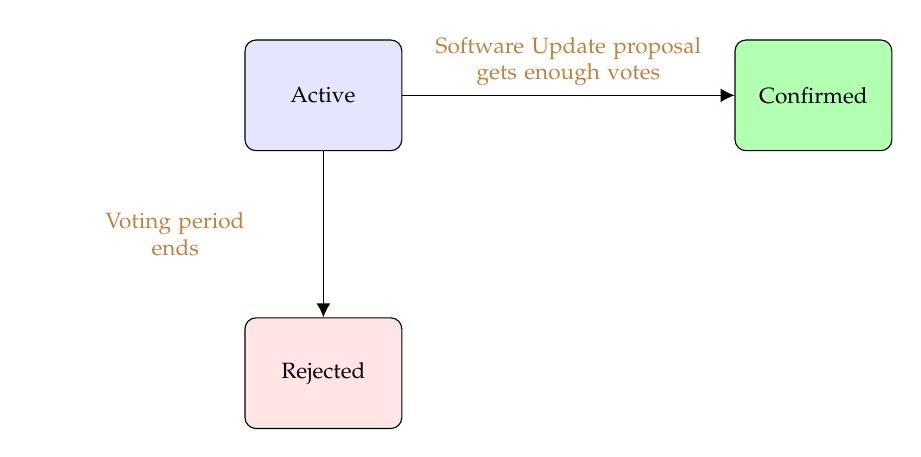
\begin{tikzpicture}[ align = center
                     , node distance = 6em and 12em
                     , text width = 5em
                     , font = \footnotesize
                     , >={Latex[width=0.5em, length=0.5em]}
                     , every node/.style = { rectangle
                                         , rounded corners
                                         , draw = black
                                         , align = center
                                         , minimum height = 4em }
                     ]

  \node (active) [fill = blue!10] {Active};
  \node (rejected) [below = of active, fill = red!10] {Rejected};
  \node (confirmed) [right = of active, fill = green!30] {Confirmed};

  \tikzset{every node/.style={align=center, text width=10em, text=brown}}

  \draw[->] (active)
  edge node [above] {Software Update proposal\\ gets enough votes}
  (confirmed);

  \draw[->] (active)
  edge node [left] {Voting period \\ends}
  (rejected);

  \end{tikzpicture}

  \caption{State-transition diagram for software-updates}
  \label{fig:st-diagram-sw-up}
\end{figure}

\clearpage

The interface rule for protocol-version endorsement makes use of the
$\trans{upend}{}$ transition, where we set the threshold for proposal adoption
to: the number of genesis keys ($\var{ngk}$) times the minimum proportion of
genesis keys that need to endorse an update proposal for it to become a
candidate for adoption (given by the protocol parameter $\var{upAdptThd}$). In
addition, the unconfirmed proposals that are older than $u$ blocks are removed
from the parts of the state that hold:
\begin{itemize}
\item the registered protocol and software update proposals,
\item the votes associated with the proposals,
\item the set of endorsement-key pairs, and
\item the block number in which proposals where added.
\end{itemize}

In Rule~\ref{eq:rule:upi-pend}, the set of proposal id's $\var{pid_{keep}}$
contains only those proposals that haven't expired yet or that are confirmed.
Once a proposal $\var{up}$ is confirmed, it is removed from the set of
confirmed proposals ($\var{cps}$) when a new a protocol version gets adopted
(see Rule~\ref{eq:rule:upi-ec-pv-change}).
%
The set of endorsement-key pairs is cleaned here as well as in the epoch change
rule (Rule~\ref{eq:rule:upi-ec-pv-change}). The reason for this is that this set grows at
each block, and it can get considerably large if no proposal gets adopted at
the end on an epoch.

\begin{figure}[htb]
  \begin{equation}
    \label{eq:rule:upi-pend}
    \inference
    {
      {
        \begin{array}{l}
          k\\
          s_n\\
          q \cdot \var{ngk}\\
          \var{dms}\\
          \var{cps}\\
          \var{rpus}
        \end{array}
      }
      \vdash
      {
        \left(
          \begin{array}{l}
            \var{fads}\\
            \var{bvs}
          \end{array}
        \right)
      }
      \trans{upend}{(\var{bv}, \var{vk})}
      {
        \left(
          \begin{array}{l}
            \var{fads'}\\
            \var{bvs'}
          \end{array}
        \right)
      }\\
      \var{stableAfter} \mapsto k \in  \var{pps}
      & \var{upropTTL} \mapsto u \in \var{pps}
      & \var{upAdptThd} \mapsto q \in \var{pps} \\
      {
        \begin{array}{r@{~\leteq~}l}
          \var{pids_{keep}} & \dom~(pws \restrictrange [s_n - u, ..]) \cup \dom~\var{cps}\\
          \var{vs_{keep}} & \dom~(\range~\var{rpus'})\\
          \var{rpus'} & \var{pids_{keep}} \restrictdom \var{rpus}
        \end{array}
      }
    }
    {
      {
        \begin{array}{l}
          s_n\\
          \var{ngk}\\
          \var{dms}
        \end{array}
      }
      \vdash
      {
        \left(
          \begin{array}{l}
            \var{e_p}\\
            (\var{pv}, \var{pps})\\
            \var{fads}\\
            \var{avs}\\
            \var{rpus}\\
            \var{raus}\\
            \var{cps}\\
            \var{vts}\\
            \var{bvs}\\
            \var{pws}
          \end{array}
        \right)
      }
      \trans{upiend}{(\var{bv}, \var{vk})}
      {
        \left(
          \begin{array}{l}
            \var{e_p}\\
            (\var{pv}, \var{pps})\\
            \var{fads'}\\
            \var{avs}\\
            \var{rpus'}\\
            \var{pids_{keep}} \restrictdom \var{raus}\\
            \var{cps}\\
            \var{pids_{keep}} \restrictdom \var{vts}\\
            \var{vs_{keep}}  \restrictdom \var{bvs'}\\
            \var{pids_{keep}} \restrictdom \var{pws}
          \end{array}
        \right)
      }
    }
  \end{equation}
  \caption{Proposal endorsement rules}
  \label{fig:rules:upi-pend}
\end{figure}

\clearpage

Rule~\ref{eq:rule:upi-ec-pv-change} models how the epoch, protocol-version and its
parameters are changed depending on the epoch in the signal ($e_n$ in this
case). A change in the epoch only occurs if the new epoch is greater than the
previously seen epoch ($e_p$).
%
On an epoch change, this rule will pick a candidate that gathered enough
endorsements at least $2 \cdot k$ slots ago. If a protocol-version candidate
cannot gather enough endorsements $2 \cdot k$ slots before the end of an
epoch, the proposal can only be adopted in the next epoch.
%
Figure~\ref{fig:up-confirmed-too-late} shows an example of a proposal being
confirmed too late in an epoch, where it is not possible to get enough
endorsements in the remaining window. In this Figure we take $k = 2$, and we
assume $4$ endorsements are needed to consider a proposal as candidate for
adoption.
%
Note that, in the final state, we use union override to define the updated
parameters ($\var{pps} \unionoverrideRight \var{pps'}$). This is because candidate
proposal might only update some parameters of the protocol.

In Rule~\ref{eq:rule:upi-ec-pv-change}, when a new proposal gets adopted, all
the state components that refer to protocol update proposals get emptied. The
reason for this is that at the moment of registering a proposal, we evaluated
it in a state where the protocol parameters that we used for this are no longer
up to date (see for instance \cref{eq:func:can-update}). For instance, assume
we register a proposal $\var{up}$ which only changes the maximum transaction
size to $x$, and the current block size is set to $x + 1$. Then,
$\fun{canUpdate}$ holds, since the maximum transaction size is less than the
maximum block size. If now a new proposal gets adopted that changes the maximum
block size to $x - 1$, then this invalidates $\var{up}$ since $\fun{canUpdate}$
no longer holds.
%

If there are no candidates for adoption, then the state variables remain
unaltered (Rule~\ref{eq:rule:upi-ec-pv-unchanged}).

Also note that the registered software-update proposals need not be cleaned
here, since this is done either when a proposal gets confirmed or when it
expires.

\begin{figure}[htb]
  \begin{equation}
    \label{eq:rule:pvbump-change-noop}
    \inference
    {
      e_n \leq e_p
    }
    {
      {\begin{array}{l}
         k\\
         s_n\\
         \var{fads}
       \end{array}}
      \vdash
      {
        \left(
          \begin{array}{l}
            \var{e_p}\\
            \var{(\var{pv}, \var{pps})}
          \end{array}
        \right)
      }
      \trans{pvbump}{\var{e_n}}
      {
        \left(
          \begin{array}{l}
            \var{e_p}\\
            \var{(\var{pv}, \var{pps})}
          \end{array}
        \right)
      }
    }
  \end{equation}
  \nextdef
  \begin{equation}
    \label{eq:rule:pvbump-change-epoch-only}
    \inference
    {
      [.., s_n - 2 \cdot k] \restrictdom \var{fads} = \epsilon &  e_p < e_n
    }
    {
      {\begin{array}{l}
         k\\
         s_n\\
         \var{fads}
       \end{array}}
      \vdash
      {
        \left(
          \begin{array}{l}
            \var{e_p}\\
            \var{(\var{pv}, \var{pps})}\\
          \end{array}
        \right)
      }
      \trans{pvbump}{\var{e_n}}
      {
        \left(
          \begin{array}{l}
            \var{e_n}\\
            \var{(\var{pv}, \var{pps})}\\
          \end{array}
        \right)
      }
    }
  \end{equation}
  \nextdef
  \begin{equation}
    \label{eq:rule:pvbump-change}
    \inference
    {
      \wcard ; (\wcard , (\var{pv_c}, \var{pps_c})) \leteq [.., s_n - 2 \cdot k] \restrictdom \var{fads}
      & e_p < e_n
    }
    {
      {\begin{array}{l}
         k\\
         s_n\\
         \var{fads}
       \end{array}}
      \vdash
      {
        \left(
          \begin{array}{l}
            \var{e_p}\\
            \var{(\var{pv}, \var{pps})}\\
          \end{array}
        \right)
      }
      \trans{pvbump}{\var{e_n}}
      {
        \left(
          \begin{array}{l}
            \var{e_n}\\
            \var{(\var{pv_c}, \var{pps_c})}\\
          \end{array}
        \right)
      }
    }
  \end{equation}
  \caption{Protocol version bump rules}
  \label{fig:rules:fads}
\end{figure}

\begin{figure}[htb]
  \begin{equation}
    \label{eq:rule:upi-ec-pv-unchanged}
    \inference
    {
      \var{stableAfter} \mapsto k \in  \var{pps} &
      {\begin{array}{l}
         k\\
         s_n\\
         \var{fads}
       \end{array}}
      \vdash
      {
        \left(
          \begin{array}{l}
            \var{e_p}\\
            \var{(\var{pv}, \var{pps})}
          \end{array}
        \right)
      }
      \trans{pvbump}{\var{e_n}}
      {
        \left(
          \begin{array}{l}
            \var{e'}\\
            \var{(\var{pv'}, \var{pps'})}\\
          \end{array}
        \right)
      }\\ ~ \\ \var{pv} = \var{pv'}
    }
    {
      {
        \begin{array}{l}
          s_n\\
          \var{ngk}\\
          \var{dms}
        \end{array}
      }
      \vdash
      {
        \left(
          \begin{array}{l}
            \var{e_p}\\
            \var{(\var{pv}, \var{pps})}\\
            \var{fads}\\
            \var{avs}\\
            \var{rpus}\\
            \var{raus}\\
            \var{cps}\\
            \var{vts}\\
            \var{bvs}\\
            \var{pws}
          \end{array}
        \right)
      }
      \trans{upiec}{\var{e_n}}
      {
        \left(
          \begin{array}{l}
            \var{e'}\\
            \var{(\var{pv}, \var{pps})}\\
            \var{fads}\\
            \var{avs}\\
            \var{rpus}\\
            \var{raus}\\
            \var{cps}\\
            \var{vts}\\
            \var{bvs}\\
            \var{pws}
          \end{array}
        \right)
      }
    }
  \end{equation}
  \nextdef
  \begin{equation}
    \label{eq:rule:upi-ec-pv-change}
    \inference
    {
      \var{stableAfter} \mapsto k \in  \var{pps} &
      {\begin{array}{l}
         k\\
         s_n\\
         \var{fads}
       \end{array}}
      \vdash
      {
        \left(
          \begin{array}{l}
            \var{e_p}\\
            \var{(\var{pv}, \var{pps})}
          \end{array}
        \right)
      }
      \trans{pvbump}{\var{e_n}}
      {
        \left(
          \begin{array}{l}
            \var{e'}\\
            \var{(\var{pv'}, \var{pps'})}\\
          \end{array}
        \right)
      }\\ ~ \\ \var{pv} \neq \var{pv'}
    }
    {
      {
        \begin{array}{l}
          s_n\\
          \var{ngk}\\
          \var{dms}
        \end{array}
      }
      \vdash
      {
        \left(
          \begin{array}{l}
            \var{e_p}\\
            \var{(\var{pv}, \var{pps})}\\
            \var{fads}\\
            \var{avs}\\
            \var{rpus}\\
            \var{raus}\\
            \var{cps}\\
            \var{vts}\\
            \var{bvs}\\
            \var{pws}
          \end{array}
        \right)
      }
      \trans{upiec}{\var{e_n}}
      {
        \left(
          \begin{array}{l}
            \var{e'}\\
            \var{(\var{pv'}, \var{pps'})}\\
            \epsilon\\
            \var{avs}\\
            \emptyset\\
            \var{raus}\\
            \emptyset\\
            \emptyset\\
            \emptyset\\
            \emptyset\\
          \end{array}
        \right)
      }
    }
  \end{equation}
  \caption{Block version adoption on epoch change rules}
  \label{fig:rules:upi-ec}
\end{figure}

\begin{figure}[htb]
  \centering
  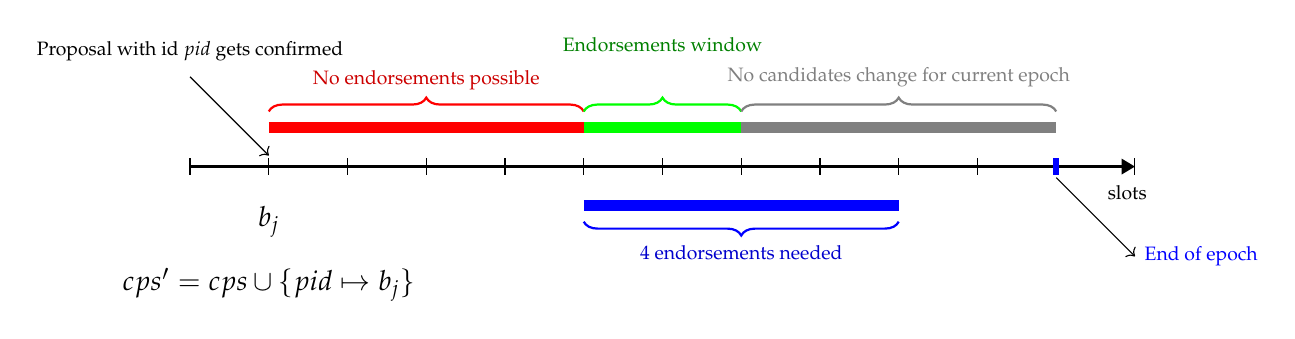
\begin{tikzpicture}
    %%
    %% Macros used in this picture
    %%
    %
    % Number of slots
    \pgfmathsetmacro{\nrSlots}{12}
    % Slot in which the proposal gets confirmed
    \pgfmathsetmacro{\cSlot}{1}
    % Our special K.
    \pgfmathsetmacro{\K}{4}
    % Epoch end.
    \pgfmathsetmacro{\eend}{11}
    % Number of positive votes needed
    \pgfmathsetmacro{\votes}{4}

    % Draw the horizontal line
    \draw[thick, -Triangle] (0,0) -- (\nrSlots,0)
    node[font=\scriptsize,below left=3pt and -8pt]{slots};

    % % draw vertical lines
    \foreach \x in {0,1,...,\nrSlots}
    \draw (\x cm, 3pt) -- (\x cm, -3pt);

    % Add a label to with the block number in which the proposal got confirmed.
    \node at (\cSlot, -.7) {$b_j$};

    % Update in cps
    \node at (\cSlot, -1.5) {$\var{cps'} = \var{cps} \cup \{ \var{pid} \mapsto b_j \}$};

    % The no-endorsements red bar.
    \draw[red, line width=4pt] (\cSlot, .5) -- +(\K, 0);

    % Brace above the no-endorsement window bar.
    \draw[thick, red, decorate, decoration={brace, amplitude=5pt}]
    (\cSlot, .7) -- +(\K, 0)
    node[black!20!red, midway, above=4pt, font=\scriptsize] {No endorsements possible};

    % The endorsements window.
    \coordinate (ewStart) at (\cSlot + \K, .5);
    \coordinate (ewEnd) at ($(\eend - \K, .5)$);
    \draw[green, line width=4pt]
    (ewStart) -- (ewEnd);

    % Brace above the endorsements window
    \coordinate (ewStartB) at ($(ewStart) + (0, 0.2)$);
    \coordinate (ewEndB) at ($(ewEnd) + (0, 0.2)$);
    \draw[thick, green, decorate, decoration={brace, amplitude=5pt}]
    (ewStartB) -- (ewEndB)
    node[black!50!green, midway, above=18pt, font=\scriptsize] {Endorsements window};

    % The no-candidates change window.
    \coordinate (nccStart) at (\eend - \K, .5);
    \coordinate (nccEnd) at ($(\eend, .5)$);
    \draw[gray, line width=4pt]
    (nccStart) -- (nccEnd);

    % Brace above the no-candidates change window.
    \coordinate (nccStartB) at ($(nccStart) + (0, 0.2)$);
    \coordinate (nccEndB) at ($(nccEnd) + (0, 0.2)$);
    \draw[thick, gray, decorate, decoration={brace, amplitude=5pt}]
    (nccStartB) -- (nccEndB)
    node[gray, midway, above=5pt, font=\scriptsize] {No candidates change for current epoch};


    % The 2k before end-of-epoch window.
    \coordinate (beeStart) at (\cSlot + \K, -.5);
    \coordinate (beeEnd) at ($(\cSlot + \K + \votes, -.5)$);
    \draw[blue, line width=4pt]
    (beeStart) -- (beeEnd);

    % Brace on above the 2k before end-of-epoch window.
    \coordinate (beeStartB) at ($(beeStart) - (0, 0.2)$);
    \coordinate (beeEndB) at ($(beeEnd) - (0, 0.2)$);
    \draw[thick, blue, decorate, decoration={brace, amplitude=5pt}]
    (beeEndB) -- (beeStartB)
    node[black!20!blue, midway, below=5pt, font=\scriptsize] {$\votes$ endorsements needed};

    \draw[blue, line width=2pt] (\eend, 3pt) -- (\eend, -3pt);

    \draw[<-] (\cSlot, 4pt) -- +(-1, 1)
    node [above=2pt, black, font=\scriptsize]
    {Proposal with id $\var{pid}$ gets confirmed};

    \draw[->] (\eend, -4pt) -- +(1, -1)
    node[right, blue, font=\scriptsize] {End of epoch};
  \end{tikzpicture}
  \caption{An update proposal confirmed too late}
  \label{fig:up-confirmed-too-late}
\end{figure}

Figure~\ref{fig:st-diagram-pt-up} shows the different states a protocol-update
proposal can be in, and what causes the transitions between them.

\begin{figure}[ht]
  \centering
  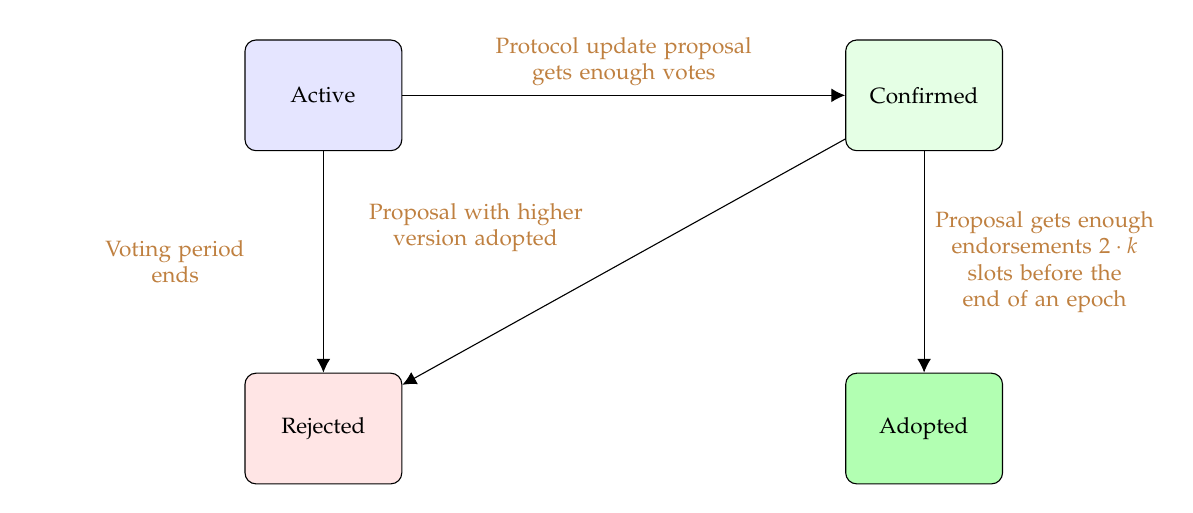
\begin{tikzpicture}[ align = center
                     , node distance = 8em and 16em
                     , text width = 5em
                     , font = \footnotesize
                     , >={Latex[width=0.5em, length=0.5em]}
                     , every node/.style = { rectangle
                                         , rounded corners
                                         , draw = black
                                         , align = center
                                         , minimum height = 4em }
                     ]

  \node (active) [fill = blue!10] {Active};
  \node (rejected) [below = of active, fill = red!10] {Rejected};
  \node (confirmed) [right = of active, fill = green!10] {Confirmed};
  \node (adopted) [below = of confirmed, fill = green!30] {Adopted};

  \tikzset{every node/.style={align=center, text width=10em, text=brown}}

  \draw[->] (active)
  edge node [above] {Protocol update proposal\\ gets enough votes}
  (confirmed);

  \draw[->] (active)
  edge node [left] {Voting period \\ends}
  (rejected);

  \draw[->] (confirmed)
  edge node [above left]
  {Proposal with higher version adopted}
  (rejected);

  \draw[->] (confirmed)
  edge node [right, text width=8em]
  {Proposal gets enough endorsements $2 \cdot k$ slots before the end of an epoch}
  (adopted);

  \end{tikzpicture}

  \caption{State-transition diagram for protocol-updates}
  \label{fig:st-diagram-pt-up}
\end{figure}

\section{Formal Properties}
\label{sec:properties}

This appendix collects the main formal properties that the new ledger rules are expected to satisfy.

\begin{enumerate}[label=P{\arabic*}:\ ]
\item
  \emph{Consistency with Shelley.}
  All formal properties that were defined for Shelley in \ref{XX} remain valid.\todo{Confirm this, or list any exceptions.}
\item
  \emph{Consistency with Multi-Asset.}
  All formal properties that were defined for multi-asset tokens in \ref{XX} also remain valid.\todo{Confirm this, or list any exceptions.}
\item
  \emph{Ada Consistency.}
  Any token with the $\PolicyID$ of Ada is an Ada token, i.e. it
  also has the $\AssetID$ of Ada.
\item
  \emph{General Accounting.}
  The \emph{general accounting} property\todo{Reference or explain this} holds for any transaction,
  whether it is fully processed or just paying fees. In particular,
  this implies that the total amount of Ada in the system is constant.
\item
  \emph{Fee Movement.}
  If a transaction is accepted and marked as paying fees only
  (i.e. $\fun{txvaltag}\, tx = \True$), then the only change to the ledger
  when processing the transaction is that the inputs marked for paying
  fees are moved to the fee pot.
\item
  \emph{Transaction Validation.}
  If a Shelley transaction is accepted, it is fully processed.\todo{What does this mean? Is this: Transaction consistency - any transaction that is successfully validated can be executed successfully by the interpreter.}
\item
  \emph{Extended UTxO Validation.}
  If a transaction extends the UTxO, all its scripts validate, and
  if it has a script that does not validate, it cannot extend the
  UTxO.
\item
  \emph{Non-Token Forging.}
  A valid transaction that does not forge tokens satisfies the
  accounting property of the Shelley ledger where the type $\Coin$ is
  replaced by $\Value$.
\item
  \todo{\emph{Script consistency.} Scripts are only processed by valid version of the interpreter.}
\item
  \todo{\emph{Backwards compatibility.} All scripts that could be processed by any previous version of the interpreter
    remain valid indefinitely.}
\item
  \todo{\emph{Cost consistency.} - no transaction exceeds the specified resource bounds.}
\item
  \todo{\emph{Backwards Compatibility.} Any transaction that was accepted in a previous version of the ledger rules
    has exactly the same cost and effect, except that the transaction output is extended.}
\item
  ... \todo{Anything else?}
\end{enumerate}


\newpage

\begin{appendix}
  \section{Proofs}
\label{sec:proofs}

\newif\ifproofs
% \proofstrue comment in to include generated proofs

For the proofs we use the automated theorem prover
MetiTarski~\cite{DBLP:journals/jar/AkbarpourP10} which is specialized for proofs
over real arithmetic, including elementary functions.

\begin{proof}
The property~(\ref{prop:minimal-refund}) (p.~\pageref{prop:minimal-refund}) for
the minimal refund can be proven automatically via

\begin{verbatim}
fof(minimal_refund, conjecture,
! [Dmin, Lambda, Delta, Dval] :
((Dmin : (=0,1=) & Lambda > 0 & Delta > 0 & Dval > 0
=>
Dval*Dmin >= 0 &
(Dval * (Dmin + (1 - Dmin) * exp(-Lambda * Delta))) : (=Dval * Dmin, Dval=)))).

fof(floor_lower_upper, conjecture,
! [X] :
(X >= 0 => X - 1 <= floor(X) & floor(X) <= X)).
\end{verbatim}
  \verb|minimal_refund| shows that the resulting value is within the interval
  $[d_{val}\cdot d_{min}, d_{val}]$ and that $d_{val}\cdot d_{min}$ is
  non-negative, while \verb|floor_lower_upper| shows that the floor of a value
  $x$ has an upper bound $x$ and lower bound $x - 1$.

\ifproofs
\begin{verbatim}
SZS output start CNFRefutation for minRefund.tptp
cnf(lgen_le_neg, axiom, (X <= Y | ~ lgen(0, X, Y))).

cnf(leq_left_divide_mul_pos, axiom, (Y * Z < X | X / Z <= Y | Z <= 0)).

cnf(interval_intro, axiom,
    (~ lgen(R, A, X) | ~ lgen(S, X, B) | interval(R, A, S, B, X))).

cnf(interval_elim1, axiom, (~ interval(R, A, S, B, X) | lgen(R, A, X))).

cnf(interval_elim2, axiom, (~ interval(R, A, S, B, X) | lgen(S, X, B))).

cnf(exp_upper_bound_cf2, axiom,
    (0 <= X | ~ lgen(R, (X ^ 2 + 6 * X + 12) / (X ^ 2 - 6 * X + 12), Y) |
     lgen(R, exp(X), Y))).

fof(minimal_refund, conjecture,
    (! [Dmin, Lambda, Delta, Dval] :
       ((interval(0, 0, 0, 1, Dmin) & 0 < Lambda & 0 < Delta & 0 < Dval) =>
        (0 <= Dval * Dmin &
         interval(0, Dval * Dmin, 0, Dval,
                  Dval * (Dmin + (1 - Dmin) * exp(-Lambda * Delta))))))).

fof(subgoal_0, plain,
    (! [Dmin, Lambda, Delta, Dval] :
       ((interval(0, 0, 0, 1, Dmin) & 0 < Lambda & 0 < Delta & 0 < Dval) =>
        0 <= Dval * Dmin)), inference(strip, [], [minimal_refund])).

fof(subgoal_1, plain,
    (! [Dmin, Lambda, Delta, Dval] :
       (((interval(0, 0, 0, 1, Dmin) & 0 < Lambda & 0 < Delta & 0 < Dval) &
         0 <= Dval * Dmin) =>
        interval(0, Dval * Dmin, 0, Dval,
                 Dval * (Dmin + (1 - Dmin) * exp(-Lambda * Delta))))),
    inference(strip, [], [minimal_refund])).

fof(negate_0_0, plain,
    (~ ! [Dmin, Lambda, Delta, Dval] :
         ((interval(0, 0, 0, 1, Dmin) & 0 < Lambda & 0 < Delta &
           0 < Dval) => 0 <= Dval * Dmin)),
    inference(negate, [], [subgoal_0])).

fof(normalize_0_0, plain,
    (? [Delta, Dmin, Dval, Lambda] :
       (0 < Delta & 0 < Dval & 0 < Lambda & Dval * Dmin < 0 &
        interval(0, 0, 0, 1, Dmin))),
    inference(canonicalize, [], [negate_0_0])).

fof(normalize_0_1, plain,
    (skoDvalC2 * skoDminC2 < 0 & 0 < skoDeltaC2 & 0 < skoDvalC2 &
     0 < skoLambdaC2 & interval(0, 0, 0, 1, skoDminC2)),
    inference(skolemize, [], [normalize_0_0])).

fof(normalize_0_2, plain, (interval(0, 0, 0, 1, skoDminC2)),
    inference(conjunct, [], [normalize_0_1])).

fof(normalize_0_3, plain, (skoDvalC2 * skoDminC2 < 0),
    inference(conjunct, [], [normalize_0_1])).

fof(normalize_0_4, plain, (0 < skoLambdaC2),
    inference(conjunct, [], [normalize_0_1])).

fof(normalize_0_5, plain, (0 < skoDvalC2),
    inference(conjunct, [], [normalize_0_1])).

fof(normalize_0_6, plain, (0 < skoDeltaC2),
    inference(conjunct, [], [normalize_0_1])).

cnf(refute_0_0, plain, (interval(0, 0, 0, 1, skoDminC2)),
    inference(canonicalize, [], [normalize_0_2])).

cnf(refute_0_1, plain,
    (~ interval(0, 0, 0, 1, skoDminC2) | lgen(0, 0, skoDminC2)),
    inference(subst, [], [interval_elim1])).

cnf(refute_0_2, plain, (lgen(0, 0, skoDminC2)),
    inference(resolve, [], [refute_0_0, refute_0_1])).

cnf(refute_0_3, plain, (0 <= skoDminC2),
    inference(arithmetic, [], [refute_0_2])).

cnf(refute_0_4, plain, (skoDvalC2 * skoDminC2 < 0),
    inference(canonicalize, [], [normalize_0_3])).

cnf(refute_0_5, plain, (0 < skoDvalC2 * (skoDminC2 * -1)),
    inference(arithmetic, [], [refute_0_4])).

cnf(refute_0_6, plain, (0 < skoLambdaC2),
    inference(canonicalize, [], [normalize_0_4])).

cnf(refute_0_7, plain, (0 < skoDvalC2),
    inference(canonicalize, [], [normalize_0_5])).

cnf(refute_0_8, plain, (0 < skoDeltaC2),
    inference(canonicalize, [], [normalize_0_6])).

cnf(refute_0_9, plain, (skoDminC2 < 0),
    inference(decision, [],
              [refute_0_5, refute_0_6, refute_0_7, refute_0_8])).

cnf(refute_0_10, plain, ($false),
    inference(resolve, [], [refute_0_3, refute_0_9])).

fof(negate_1_0, plain,
    (~ ! [Dmin, Lambda, Delta, Dval] :
         (((interval(0, 0, 0, 1, Dmin) & 0 < Lambda & 0 < Delta &
            0 < Dval) & 0 <= Dval * Dmin) =>
          interval(0, Dval * Dmin, 0, Dval,
                   Dval * (Dmin + (1 - Dmin) * exp(-Lambda * Delta))))),
    inference(negate, [], [subgoal_1])).

fof(normalize_1_0, plain,
    (? [Delta, Dmin, Dval, Lambda] :
       (0 < Delta & 0 < Dval & 0 < Lambda &
        ~ interval(0, Dval * Dmin, 0, Dval,
                   Dval * (Dmin + (1 - Dmin) * exp(-Lambda * Delta))) &
        0 <= Dval * Dmin & interval(0, 0, 0, 1, Dmin))),
    inference(canonicalize, [], [negate_1_0])).

fof(normalize_1_1, plain,
    (0 < skoDeltaC3 & 0 < skoDvalC3 & 0 < skoLambdaC3 &
     ~ interval(0, skoDvalC3 * skoDminC3, 0, skoDvalC3,
                skoDvalC3 *
                (skoDminC3 +
                 (1 - skoDminC3) * exp(-skoLambdaC3 * skoDeltaC3))) &
     0 <= skoDvalC3 * skoDminC3 & interval(0, 0, 0, 1, skoDminC3)),
    inference(skolemize, [], [normalize_1_0])).

fof(normalize_1_2, plain,
    (~ interval(0, skoDvalC3 * skoDminC3, 0, skoDvalC3,
                skoDvalC3 *
                (skoDminC3 +
                 (1 - skoDminC3) * exp(-skoLambdaC3 * skoDeltaC3)))),
    inference(conjunct, [], [normalize_1_1])).

fof(normalize_1_3, plain, (interval(0, 0, 0, 1, skoDminC3)),
    inference(conjunct, [], [normalize_1_1])).

fof(normalize_1_4, plain, (0 <= skoDvalC3 * skoDminC3),
    inference(conjunct, [], [normalize_1_1])).

fof(normalize_1_5, plain, (0 < skoLambdaC3),
    inference(conjunct, [], [normalize_1_1])).

fof(normalize_1_6, plain, (0 < skoDvalC3),
    inference(conjunct, [], [normalize_1_1])).

fof(normalize_1_7, plain, (0 < skoDeltaC3),
    inference(conjunct, [], [normalize_1_1])).

cnf(refute_1_0, plain,
    (1 *
     (12 +
      skoLambdaC3 *
      (skoDeltaC3 * 6 + skoLambdaC3 * (skoDeltaC3 * skoDeltaC3))) <
     12 +
     skoLambdaC3 *
     (skoDeltaC3 * -6 + skoLambdaC3 * (skoDeltaC3 * skoDeltaC3)) |
     12 +
     skoLambdaC3 *
     (skoDeltaC3 * 6 + skoLambdaC3 * (skoDeltaC3 * skoDeltaC3)) <= 0 |
     (12 +
      skoLambdaC3 *
      (skoDeltaC3 * -6 + skoLambdaC3 * (skoDeltaC3 * skoDeltaC3))) /
     (12 +
      skoLambdaC3 *
      (skoDeltaC3 * 6 + skoLambdaC3 * (skoDeltaC3 * skoDeltaC3))) <= 1),
    inference(subst, [], [leq_left_divide_mul_pos])).

cnf(refute_1_1, plain,
    (~ lgen(0, exp(X_000190), X_000191) | exp(X_000190) <= X_000191),
    inference(subst, [], [lgen_le_neg])).

cnf(refute_1_2, plain,
    (~ lgen(0,
            (X_000190 ^ 2 + 6 * X_000190 + 12) /
            (X_000190 ^ 2 - 6 * X_000190 + 12), X_000191) | 0 <= X_000190 |
     lgen(0, exp(X_000190), X_000191)),
    inference(subst, [], [exp_upper_bound_cf2])).

cnf(refute_1_3, plain,
    (~ lgen(0,
            (X_000190 ^ 2 + 6 * X_000190 + 12) /
            (X_000190 ^ 2 - 6 * X_000190 + 12), X_000191) | 0 <= X_000190 |
     exp(X_000190) <= X_000191),
    inference(resolve, [], [refute_1_2, refute_1_1])).

cnf(refute_1_4, plain,
    (X_000191 <
     (12 + X_000190 * (6 + X_000190)) / (12 + X_000190 * (-6 + X_000190)) |
     0 <= X_000190 | exp(X_000190) <= X_000191),
    inference(arithmetic, [], [refute_1_3])).

cnf(refute_1_5, plain,
    (1 <
     (12 +
      skoLambdaC3 * (skoDeltaC3 * -1) *
      (6 + skoLambdaC3 * (skoDeltaC3 * -1))) /
     (12 +
      skoLambdaC3 * (skoDeltaC3 * -1) *
      (-6 + skoLambdaC3 * (skoDeltaC3 * -1))) |
     0 <= skoLambdaC3 * (skoDeltaC3 * -1) |
     exp(skoLambdaC3 * (skoDeltaC3 * -1)) <= 1),
    inference(subst, [], [refute_1_4])).

cnf(refute_1_6, plain,
    (~ interval(0, skoDvalC3 * skoDminC3, 0, skoDvalC3,
                skoDvalC3 *
                (skoDminC3 +
                 (1 - skoDminC3) * exp(-skoLambdaC3 * skoDeltaC3)))),
    inference(canonicalize, [], [normalize_1_2])).

cnf(refute_1_7, plain,
    (~ interval(0, skoDvalC3 * skoDminC3, 0, skoDvalC3,
                skoDvalC3 * skoDminC3 +
                exp(skoLambdaC3 * (skoDeltaC3 * -1)) *
                (skoDvalC3 * (1 + skoDminC3 * -1)))),
    inference(arithmetic, [], [refute_1_6])).

cnf(refute_1_8, plain,
    (~ lgen(0, skoDvalC3 * skoDminC3,
            skoDvalC3 * skoDminC3 +
            exp(skoLambdaC3 * (skoDeltaC3 * -1)) *
            (skoDvalC3 * (1 + skoDminC3 * -1))) |
     ~ lgen(0,
            skoDvalC3 * skoDminC3 +
            exp(skoLambdaC3 * (skoDeltaC3 * -1)) *
            (skoDvalC3 * (1 + skoDminC3 * -1)), skoDvalC3) |
     interval(0, skoDvalC3 * skoDminC3, 0, skoDvalC3,
              skoDvalC3 * skoDminC3 +
              exp(skoLambdaC3 * (skoDeltaC3 * -1)) *
              (skoDvalC3 * (1 + skoDminC3 * -1)))),
    inference(subst, [], [interval_intro])).

cnf(refute_1_9, plain,
    (~ lgen(0, skoDvalC3 * skoDminC3,
            skoDvalC3 * skoDminC3 +
            exp(skoLambdaC3 * (skoDeltaC3 * -1)) *
            (skoDvalC3 * (1 + skoDminC3 * -1))) |
     ~ lgen(0,
            skoDvalC3 * skoDminC3 +
            exp(skoLambdaC3 * (skoDeltaC3 * -1)) *
            (skoDvalC3 * (1 + skoDminC3 * -1)), skoDvalC3)),
    inference(resolve, [], [refute_1_8, refute_1_7])).

cnf(refute_1_10, plain,
    (0 <
     exp(skoLambdaC3 * (skoDeltaC3 * -1)) *
     (skoDvalC3 * (-1 + skoDminC3)) |
     skoDvalC3 * (1 + skoDminC3 * -1) <
     exp(skoLambdaC3 * (skoDeltaC3 * -1)) *
     (skoDvalC3 * (1 + skoDminC3 * -1))),
    inference(arithmetic, [], [refute_1_9])).

cnf(refute_1_11, plain,
    (0 <
     exp(skoLambdaC3 * (skoDeltaC3 * -1)) *
     (skoDvalC3 * (-1 + skoDminC3)) |
     exp(skoLambdaC3 * (skoDeltaC3 * -1)) *
     (skoDvalC3 * (-1 + skoDminC3)) <= 0),
    introduced(tautology, [assume])).

cnf(refute_1_12, plain,
    (0 < 0 | skoDvalC3 * (-1 + skoDminC3) < 0 |
     0 < skoDvalC3 * (-1 + skoDminC3) |
     exp(skoLambdaC3 * (skoDeltaC3 * -1)) *
     (skoDvalC3 * (-1 + skoDminC3)) <= 0),
    inference(split, [], [refute_1_11])).

cnf(refute_1_13, plain,
    (0 < skoDvalC3 * (-1 + skoDminC3) |
     0 < skoDvalC3 * (1 + skoDminC3 * -1) |
     exp(skoLambdaC3 * (skoDeltaC3 * -1)) *
     (skoDvalC3 * (-1 + skoDminC3)) <= 0),
    inference(arithmetic, [], [refute_1_12])).

cnf(refute_1_14, plain,
    (exp(skoLambdaC3 * (skoDeltaC3 * -1)) <
     0 / (skoDvalC3 * (-1 + skoDminC3)) |
     0 <= skoDvalC3 * (-1 + skoDminC3) |
     exp(skoLambdaC3 * (skoDeltaC3 * -1)) *
     (skoDvalC3 * (-1 + skoDminC3)) <= 0),
    inference(split, [], [refute_1_11])).

cnf(refute_1_15, plain,
    (exp(skoLambdaC3 * (skoDeltaC3 * -1)) *
     (skoDvalC3 * (-1 + skoDminC3)) <= 0 |
     skoDvalC3 * (1 + skoDminC3 * -1) <= 0),
    inference(arithmetic, [], [refute_1_14])).

cnf(refute_1_16, plain,
    (0 < skoDvalC3 * (-1 + skoDminC3) |
     exp(skoLambdaC3 * (skoDeltaC3 * -1)) *
     (skoDvalC3 * (-1 + skoDminC3)) <= 0),
    inference(resolve, [], [refute_1_15, refute_1_13])).

cnf(refute_1_17, plain, (interval(0, 0, 0, 1, skoDminC3)),
    inference(canonicalize, [], [normalize_1_3])).

cnf(refute_1_18, plain,
    (~ interval(0, 0, 0, 1, skoDminC3) | lgen(0, skoDminC3, 1)),
    inference(subst, [], [interval_elim2])).

cnf(refute_1_19, plain, (lgen(0, skoDminC3, 1)),
    inference(resolve, [], [refute_1_17, refute_1_18])).

cnf(refute_1_20, plain, (skoDminC3 <= 1),
    inference(arithmetic, [], [refute_1_19])).

cnf(refute_1_21, plain, (0 <= skoDvalC3 * skoDminC3),
    inference(canonicalize, [], [normalize_1_4])).

cnf(refute_1_22, plain, (skoDvalC3 * (skoDminC3 * -1) <= 0),
    inference(arithmetic, [], [refute_1_21])).

cnf(refute_1_23, plain, (0 < skoLambdaC3),
    inference(canonicalize, [], [normalize_1_5])).

cnf(refute_1_24, plain, (0 < skoDvalC3),
    inference(canonicalize, [], [normalize_1_6])).

cnf(refute_1_25, plain, (0 < skoDeltaC3),
    inference(canonicalize, [], [normalize_1_7])).

cnf(refute_1_26, plain, (skoDvalC3 * (-1 + skoDminC3) <= 0),
    inference(decision, [],
              [refute_1_20, refute_1_22, refute_1_23, refute_1_24,
               refute_1_25])).

cnf(refute_1_27, plain,
    (exp(skoLambdaC3 * (skoDeltaC3 * -1)) *
     (skoDvalC3 * (-1 + skoDminC3)) <= 0),
    inference(resolve, [], [refute_1_26, refute_1_16])).

cnf(refute_1_28, plain,
    (skoDvalC3 * (1 + skoDminC3 * -1) <
     exp(skoLambdaC3 * (skoDeltaC3 * -1)) *
     (skoDvalC3 * (1 + skoDminC3 * -1))),
    inference(resolve, [], [refute_1_27, refute_1_10])).

cnf(refute_1_29, plain,
    (skoDvalC3 * (1 + skoDminC3 * -1) /
     (skoDvalC3 * (1 + skoDminC3 * -1)) <
     exp(skoLambdaC3 * (skoDeltaC3 * -1)) |
     skoDvalC3 * (1 + skoDminC3 * -1) <= 0),
    inference(split, [], [refute_1_28])).

cnf(refute_1_30, plain,
    (1 < exp(skoLambdaC3 * (skoDeltaC3 * -1)) |
     skoDvalC3 * (1 + skoDminC3 * -1) <= 0 | 1 = skoDminC3 |
     skoDvalC3 = 0), inference(arithmetic, [], [refute_1_29])).

cnf(refute_1_31, plain,
    (0 < skoDvalC3 * (1 + skoDminC3 * -1) | 1 = skoDminC3 | skoDvalC3 = 0),
    inference(decision, [],
              [refute_1_25, refute_1_24, refute_1_23, refute_1_22,
               refute_1_20])).

cnf(refute_1_32, plain,
    (1 < exp(skoLambdaC3 * (skoDeltaC3 * -1)) | 1 = skoDminC3 |
     skoDvalC3 = 0), inference(resolve, [], [refute_1_30, refute_1_31])).

cnf(refute_1_33, plain, (skoDvalC3 != 0 | 1 = skoDminC3),
    inference(decision, [],
              [refute_1_25, refute_1_24, refute_1_23, refute_1_22,
               refute_1_20])).

cnf(refute_1_34, plain,
    (1 < exp(skoLambdaC3 * (skoDeltaC3 * -1)) | 1 = skoDminC3),
    inference(resolve, [], [refute_1_32, refute_1_33])).

cnf(refute_1_35, plain,
    (1 <
     (12 +
      skoLambdaC3 * (skoDeltaC3 * -1) *
      (6 + skoLambdaC3 * (skoDeltaC3 * -1))) /
     (12 +
      skoLambdaC3 * (skoDeltaC3 * -1) *
      (-6 + skoLambdaC3 * (skoDeltaC3 * -1))) |
     0 <= skoLambdaC3 * (skoDeltaC3 * -1) | 1 = skoDminC3),
    inference(resolve, [], [refute_1_5, refute_1_34])).

cnf(refute_1_36, plain,
    (1 <
     (12 +
      skoLambdaC3 *
      (skoDeltaC3 * -6 + skoLambdaC3 * (skoDeltaC3 * skoDeltaC3))) /
     (12 +
      skoLambdaC3 *
      (skoDeltaC3 * 6 + skoLambdaC3 * (skoDeltaC3 * skoDeltaC3))) |
     skoLambdaC3 * skoDeltaC3 <= 0 | 1 = skoDminC3),
    inference(arithmetic, [], [refute_1_35])).

cnf(refute_1_37, plain,
    (skoDvalC3 * (1 + skoDminC3 * -1) < 0 |
     0 < skoDvalC3 * (1 + skoDminC3 * -1)),
    inference(split, [], [refute_1_28])).

cnf(refute_1_38, plain,
    (0 < skoDvalC3 * (-1 + skoDminC3) |
     0 < skoDvalC3 * (1 + skoDminC3 * -1)),
    inference(arithmetic, [], [refute_1_37])).

cnf(refute_1_39, plain,
    (0 < skoDvalC3 * (1 + skoDminC3 * -1) |
     skoDvalC3 * (-1 + skoDminC3) <= 0),
    inference(decision, [],
              [refute_1_25, refute_1_24, refute_1_23, refute_1_22,
               refute_1_20])).

cnf(refute_1_40, plain, (0 < skoDvalC3 * (1 + skoDminC3 * -1)),
    inference(resolve, [], [refute_1_39, refute_1_38])).

cnf(refute_1_41, plain, (0 < skoLambdaC3 * skoDeltaC3 | 1 = skoDminC3),
    inference(decision, [],
              [refute_1_40, refute_1_25, refute_1_24, refute_1_23,
               refute_1_22, refute_1_20])).

cnf(refute_1_42, plain,
    (1 <
     (12 +
      skoLambdaC3 *
      (skoDeltaC3 * -6 + skoLambdaC3 * (skoDeltaC3 * skoDeltaC3))) /
     (12 +
      skoLambdaC3 *
      (skoDeltaC3 * 6 + skoLambdaC3 * (skoDeltaC3 * skoDeltaC3))) |
     1 = skoDminC3), inference(resolve, [], [refute_1_36, refute_1_41])).

cnf(refute_1_43, plain, (1 != skoDminC3),
    inference(decision, [],
              [refute_1_40, refute_1_25, refute_1_24, refute_1_23,
               refute_1_22, refute_1_20])).

cnf(refute_1_44, plain,
    (1 <
     (12 +
      skoLambdaC3 *
      (skoDeltaC3 * -6 + skoLambdaC3 * (skoDeltaC3 * skoDeltaC3))) /
     (12 +
      skoLambdaC3 *
      (skoDeltaC3 * 6 + skoLambdaC3 * (skoDeltaC3 * skoDeltaC3)))),
    inference(resolve, [], [refute_1_42, refute_1_43])).

cnf(refute_1_45, plain,
    (1 *
     (12 +
      skoLambdaC3 *
      (skoDeltaC3 * 6 + skoLambdaC3 * (skoDeltaC3 * skoDeltaC3))) <
     12 +
     skoLambdaC3 *
     (skoDeltaC3 * -6 + skoLambdaC3 * (skoDeltaC3 * skoDeltaC3)) |
     12 +
     skoLambdaC3 *
     (skoDeltaC3 * 6 + skoLambdaC3 * (skoDeltaC3 * skoDeltaC3)) <= 0),
    inference(resolve, [], [refute_1_0, refute_1_44])).

cnf(refute_1_46, plain,
    (0 < skoLambdaC3 * (skoDeltaC3 * -12) |
     skoLambdaC3 *
     (skoDeltaC3 * 6 + skoLambdaC3 * (skoDeltaC3 * skoDeltaC3)) <= -12),
    inference(arithmetic, [], [refute_1_45])).

cnf(refute_1_47, plain,
    (0 < skoLambdaC3 * (skoDeltaC3 * -12) |
     -12 <
     skoLambdaC3 *
     (skoDeltaC3 * 6 + skoLambdaC3 * (skoDeltaC3 * skoDeltaC3))),
    inference(decision, [],
              [refute_1_40, refute_1_25, refute_1_24, refute_1_23,
               refute_1_22, refute_1_20])).

cnf(refute_1_48, plain, (0 < skoLambdaC3 * (skoDeltaC3 * -12)),
    inference(resolve, [], [refute_1_46, refute_1_47])).

cnf(refute_1_49, plain, (skoLambdaC3 * (skoDeltaC3 * -12) <= 0),
    inference(decision, [],
              [refute_1_40, refute_1_25, refute_1_24, refute_1_23,
               refute_1_22, refute_1_20])).

cnf(refute_1_50, plain, ($false),
    inference(resolve, [], [refute_1_49, refute_1_48])).
SZS output end CNFRefutation for minRefund.tptp
\end{verbatim}

\begin{verbatim}
SZS output start CNFRefutation for floor.tptp
cnf(lgen_le_neg, axiom, (X <= Y | ~ lgen(0, X, Y))).

cnf(floor_upper_bound, axiom, (~ lgen(R, X, Y) | lgen(R, floor(X), Y))).

cnf(floor_lower_bound, axiom, (X - 1 < Y | lgen(R, Y, floor(X)))).

fof(floor_lower_upper, conjecture,
    (! [X] : (0 <= X => (X - 1 <= floor(X) & floor(X) <= X)))).

fof(subgoal_0, plain, (! [X] : (0 <= X => X - 1 <= floor(X))),
    inference(strip, [], [floor_lower_upper])).

fof(subgoal_1, plain,
    (! [X] : ((0 <= X & X - 1 <= floor(X)) => floor(X) <= X)),
    inference(strip, [], [floor_lower_upper])).

fof(negate_0_0, plain, (~ ! [X] : (0 <= X => X - 1 <= floor(X))),
    inference(negate, [], [subgoal_0])).

fof(normalize_0_0, plain, (? [X] : (floor(X) < X - 1 & 0 <= X)),
    inference(canonicalize, [], [negate_0_0])).

fof(normalize_0_1, plain, (floor(skoXC2) < skoXC2 - 1 & 0 <= skoXC2),
    inference(skolemize, [], [normalize_0_0])).

fof(normalize_0_2, plain, (floor(skoXC2) < skoXC2 - 1),
    inference(conjunct, [], [normalize_0_1])).

cnf(refute_0_0, plain, (floor(skoXC2) < skoXC2 - 1),
    inference(canonicalize, [], [normalize_0_2])).

cnf(refute_0_1, plain, (floor(skoXC2) < -1 + skoXC2),
    inference(arithmetic, [], [refute_0_0])).

cnf(refute_0_2, plain,
    (~ lgen(0, X_000012, floor(X_000011)) | X_000012 <= floor(X_000011)),
    inference(subst, [], [lgen_le_neg])).

cnf(refute_0_3, plain,
    (X_000011 - 1 < X_000012 | lgen(0, X_000012, floor(X_000011))),
    inference(subst, [], [floor_lower_bound])).

cnf(refute_0_4, plain,
    (X_000011 - 1 < X_000012 | X_000012 <= floor(X_000011)),
    inference(resolve, [], [refute_0_3, refute_0_2])).

cnf(refute_0_5, plain,
    (-1 + X_000011 < X_000012 | X_000012 <= floor(X_000011)),
    inference(arithmetic, [], [refute_0_4])).

cnf(refute_0_6, plain,
    (-1 + skoXC2 < -1 + skoXC2 | -1 + skoXC2 <= floor(skoXC2)),
    inference(subst, [], [refute_0_5])).

cnf(refute_0_7, plain, (-1 + skoXC2 < -1 + skoXC2),
    inference(resolve, [], [refute_0_6, refute_0_1])).

cnf(refute_0_8, plain, ($false), inference(arithmetic, [], [refute_0_7])).

fof(negate_1_0, plain,
    (~ ! [X] : ((0 <= X & X - 1 <= floor(X)) => floor(X) <= X)),
    inference(negate, [], [subgoal_1])).

fof(normalize_1_0, plain,
    (? [X] : (X < floor(X) & 0 <= X & X - 1 <= floor(X))),
    inference(canonicalize, [], [negate_1_0])).

fof(normalize_1_1, plain,
    (skoXC3 < floor(skoXC3) & 0 <= skoXC3 & skoXC3 - 1 <= floor(skoXC3)),
    inference(skolemize, [], [normalize_1_0])).

fof(normalize_1_2, plain, (skoXC3 < floor(skoXC3)),
    inference(conjunct, [], [normalize_1_1])).

cnf(refute_1_0, plain, (skoXC3 < floor(skoXC3)),
    inference(canonicalize, [], [normalize_1_2])).

cnf(refute_1_1, plain,
    (~ lgen(0, floor(X_000034), X_000035) | floor(X_000034) <= X_000035),
    inference(subst, [], [lgen_le_neg])).

cnf(refute_1_2, plain,
    (~ lgen(0, X_000034, X_000035) | lgen(0, floor(X_000034), X_000035)),
    inference(subst, [], [floor_upper_bound])).

cnf(refute_1_3, plain,
    (~ lgen(0, X_000034, X_000035) | floor(X_000034) <= X_000035),
    inference(resolve, [], [refute_1_2, refute_1_1])).

cnf(refute_1_4, plain, (X_000035 < X_000034 | floor(X_000034) <= X_000035),
    inference(arithmetic, [], [refute_1_3])).

cnf(refute_1_5, plain, (skoXC3 < skoXC3 | floor(skoXC3) <= skoXC3),
    inference(subst, [], [refute_1_4])).

cnf(refute_1_6, plain, (skoXC3 < skoXC3),
    inference(resolve, [], [refute_1_5, refute_1_0])).

cnf(refute_1_7, plain, ($false), inference(arithmetic, [], [refute_1_6])).
SZS output end CNFRefutation for floor.tptp
\end{verbatim}
\fi
\end{proof}

\begin{proof}
  The property~(\ref{prop:exponential-moving-average})
  (p.~\pageref{prop:exponential-moving-average}) for the bounded moving average
  can be proven automatically via

\begin{verbatim}
fof(simple_moving_average, conjecture,
! [Alpha, Prev, N, Nexpected] :
(Alpha : (=0, 1=) & N >= 0 & Nexpected >= 0 & Prev >= 0
=>
0 <= N/max(Nexpected, 1) &
N/max(Nexpected, 1) <= N &
Alpha*N/max(Nexpected, 1) + (1 - Alpha) * Prev <= max(Prev, N/max(Nexpected, 1)) &
min(Prev, N/max(Nexpected, 1)) <= Alpha*N/max(Nexpected, 1) + (1 - Alpha) * Prev)).
\end{verbatim}

  \ifproofs
\begin{verbatim}
SZS output start CNFRefutation for simpleMovingAvg.tptp
cnf(leq_left_divide_mul_pos, axiom, (Y * Z < X | X / Z <= Y | Z <= 0)).

cnf(leq_right_divide_mul_pos, axiom, (Y < X * Z | X <= Y / Z | Z <= 0)).

cnf(leq_right_mul_divide_pos, axiom, (Y < X / Z | X <= Y * Z | Z <= 0)).

cnf(interval_elim1, axiom, (~ interval(R, A, S, B, X) | lgen(R, A, X))).

cnf(interval_elim2, axiom, (~ interval(R, A, S, B, X) | lgen(S, X, B))).

cnf(max_1, axiom, (X < Y | max(X, Y) = X)).

cnf(max_2, axiom, (Y <= X | max(X, Y) = Y)).

cnf(min_1, axiom, (X < Y | min(X, Y) = Y)).

cnf(min_2, axiom, (Y <= X | min(X, Y) = X)).

fof(simple_moving_average, conjecture,
    (! [Alpha, Prev, N, Nexpected] :
       ((interval(0, 0, 0, 1, Alpha) & 0 <= N & 0 <= Nexpected &
         0 <= Prev) =>
        (0 <= N / max(Nexpected, 1) & N / max(Nexpected, 1) <= N &
         Alpha * N / max(Nexpected, 1) + (1 - Alpha) * Prev <=
         max(Prev, N / max(Nexpected, 1)) &
         min(Prev, N / max(Nexpected, 1)) <=
         Alpha * N / max(Nexpected, 1) + (1 - Alpha) * Prev)))).

fof(subgoal_0, plain,
    (! [Alpha, Prev, N, Nexpected] :
       ((interval(0, 0, 0, 1, Alpha) & 0 <= N & 0 <= Nexpected &
         0 <= Prev) => 0 <= N / max(Nexpected, 1))),
    inference(strip, [], [simple_moving_average])).

fof(subgoal_1, plain,
    (! [Alpha, Prev, N, Nexpected] :
       (((interval(0, 0, 0, 1, Alpha) & 0 <= N & 0 <= Nexpected &
          0 <= Prev) & 0 <= N / max(Nexpected, 1)) =>
        N / max(Nexpected, 1) <= N)),
    inference(strip, [], [simple_moving_average])).

fof(subgoal_2, plain,
    (! [Alpha, Prev, N, Nexpected] :
       (((interval(0, 0, 0, 1, Alpha) & 0 <= N & 0 <= Nexpected &
          0 <= Prev) & 0 <= N / max(Nexpected, 1) &
         N / max(Nexpected, 1) <= N) =>
        Alpha * N / max(Nexpected, 1) + (1 - Alpha) * Prev <=
        max(Prev, N / max(Nexpected, 1)))),
    inference(strip, [], [simple_moving_average])).

fof(subgoal_3, plain,
    (! [Alpha, Prev, N, Nexpected] :
       (((interval(0, 0, 0, 1, Alpha) & 0 <= N & 0 <= Nexpected &
          0 <= Prev) & 0 <= N / max(Nexpected, 1) &
         N / max(Nexpected, 1) <= N &
         Alpha * N / max(Nexpected, 1) + (1 - Alpha) * Prev <=
         max(Prev, N / max(Nexpected, 1))) =>
        min(Prev, N / max(Nexpected, 1)) <=
        Alpha * N / max(Nexpected, 1) + (1 - Alpha) * Prev)),
    inference(strip, [], [simple_moving_average])).

fof(negate_0_0, plain,
    (~ ! [Alpha, Prev, N, Nexpected] :
         ((interval(0, 0, 0, 1, Alpha) & 0 <= N & 0 <= Nexpected &
           0 <= Prev) => 0 <= N / max(Nexpected, 1))),
    inference(negate, [], [subgoal_0])).

fof(normalize_0_0, plain,
    (? [Alpha, N, Nexpected, Prev] :
       (N / max(Nexpected, 1) < 0 & 0 <= N & 0 <= Nexpected & 0 <= Prev &
        interval(0, 0, 0, 1, Alpha))),
    inference(canonicalize, [], [negate_0_0])).

fof(normalize_0_1, plain,
    (skoNC4 / max(skoNexpectedC4, 1) < 0 & 0 <= skoNC4 &
     0 <= skoNexpectedC4 & 0 <= skoPrevC4 &
     interval(0, 0, 0, 1, skoAlphaC4)),
    inference(skolemize, [], [normalize_0_0])).

fof(normalize_0_2, plain, (skoNC4 / max(skoNexpectedC4, 1) < 0),
    inference(conjunct, [], [normalize_0_1])).

fof(normalize_0_3, plain, (0 <= skoPrevC4),
    inference(conjunct, [], [normalize_0_1])).

fof(normalize_0_4, plain, (0 <= skoNexpectedC4),
    inference(conjunct, [], [normalize_0_1])).

fof(normalize_0_5, plain, (0 <= skoNC4),
    inference(conjunct, [], [normalize_0_1])).

cnf(refute_0_0, plain, (skoNC4 / max(skoNexpectedC4, 1) < 0),
    inference(canonicalize, [], [normalize_0_2])).

cnf(refute_0_1, plain,
    (skoNexpectedC4 < 1 | max(skoNexpectedC4, 1) = skoNexpectedC4),
    inference(subst, [], [max_1])).

cnf(refute_0_2, plain,
    (skoNC4 / skoNexpectedC4 < 0 |
     max(skoNexpectedC4, 1) != skoNexpectedC4 |
     0 <= skoNC4 / max(skoNexpectedC4, 1)),
    introduced(tautology, [equality])).

cnf(refute_0_3, plain,
    (skoNC4 / skoNexpectedC4 < 0 | skoNexpectedC4 < 1 |
     0 <= skoNC4 / max(skoNexpectedC4, 1)),
    inference(resolve, [], [refute_0_1, refute_0_2])).

cnf(refute_0_4, plain, (skoNC4 / skoNexpectedC4 < 0 | skoNexpectedC4 < 1),
    inference(resolve, [], [refute_0_3, refute_0_0])).

cnf(refute_0_5, plain,
    (skoNC4 < 0 * skoNexpectedC4 | 0 <= skoNC4 / skoNexpectedC4 |
     skoNexpectedC4 <= 0),
    inference(subst, [], [leq_right_divide_mul_pos])).

cnf(refute_0_6, plain,
    (skoNexpectedC4 < 1 | skoNC4 < 0 * skoNexpectedC4 |
     skoNexpectedC4 <= 0),
    inference(resolve, [], [refute_0_5, refute_0_4])).

cnf(refute_0_7, plain,
    (skoNC4 < 0 | skoNexpectedC4 < 1 | skoNexpectedC4 <= 0),
    inference(arithmetic, [], [refute_0_6])).

cnf(refute_0_8, plain, (1 <= skoNexpectedC4 | max(skoNexpectedC4, 1) = 1),
    inference(subst, [], [max_2])).

cnf(refute_0_9, plain,
    (skoNC4 / 1 < 0 | max(skoNexpectedC4, 1) != 1 |
     0 <= skoNC4 / max(skoNexpectedC4, 1)),
    introduced(tautology, [equality])).

cnf(refute_0_10, plain,
    (skoNC4 / 1 < 0 | 0 <= skoNC4 / max(skoNexpectedC4, 1) |
     1 <= skoNexpectedC4),
    inference(resolve, [], [refute_0_8, refute_0_9])).

cnf(refute_0_11, plain, (skoNC4 / 1 < 0 | 1 <= skoNexpectedC4),
    inference(resolve, [], [refute_0_10, refute_0_0])).

cnf(refute_0_12, plain, (skoNC4 < 0 | 1 <= skoNexpectedC4),
    inference(arithmetic, [], [refute_0_11])).

cnf(refute_0_13, plain, (0 <= skoPrevC4),
    inference(canonicalize, [], [normalize_0_3])).

cnf(refute_0_14, plain, (0 <= skoNexpectedC4),
    inference(canonicalize, [], [normalize_0_4])).

cnf(refute_0_15, plain, (0 <= skoNC4),
    inference(canonicalize, [], [normalize_0_5])).

cnf(refute_0_16, plain, (0 <= skoNC4 | 1 <= skoNexpectedC4),
    inference(decision, [], [refute_0_13, refute_0_14, refute_0_15])).

cnf(refute_0_17, plain, (1 <= skoNexpectedC4),
    inference(resolve, [], [refute_0_16, refute_0_12])).

cnf(refute_0_18, plain,
    (skoNexpectedC4 < 1 | 0 <= skoNC4 | skoNexpectedC4 <= 0),
    inference(decision, [],
              [refute_0_17, refute_0_13, refute_0_14, refute_0_15])).

cnf(refute_0_19, plain, (skoNexpectedC4 < 1 | skoNexpectedC4 <= 0),
    inference(resolve, [], [refute_0_18, refute_0_7])).

cnf(refute_0_20, plain, (1 <= skoNexpectedC4 | skoNexpectedC4 <= 0),
    inference(decision, [],
              [refute_0_17, refute_0_13, refute_0_14, refute_0_15])).

cnf(refute_0_21, plain, (skoNexpectedC4 <= 0),
    inference(resolve, [], [refute_0_20, refute_0_19])).

cnf(refute_0_22, plain, (0 < skoNexpectedC4),
    inference(decision, [],
              [refute_0_17, refute_0_13, refute_0_14, refute_0_15])).

cnf(refute_0_23, plain, ($false),
    inference(resolve, [], [refute_0_21, refute_0_22])).

fof(negate_1_0, plain,
    (~ ! [Alpha, Prev, N, Nexpected] :
         (((interval(0, 0, 0, 1, Alpha) & 0 <= N & 0 <= Nexpected &
            0 <= Prev) & 0 <= N / max(Nexpected, 1)) =>
          N / max(Nexpected, 1) <= N)),
    inference(negate, [], [subgoal_1])).

fof(normalize_1_0, plain,
    (? [Alpha, N, Nexpected, Prev] :
       (N < N / max(Nexpected, 1) & 0 <= N & 0 <= Nexpected & 0 <= Prev &
        0 <= N / max(Nexpected, 1) & interval(0, 0, 0, 1, Alpha))),
    inference(canonicalize, [], [negate_1_0])).

fof(normalize_1_1, plain,
    (skoNC5 < skoNC5 / max(skoNexpectedC5, 1) &
     0 <= skoNC5 / max(skoNexpectedC5, 1) & 0 <= skoNC5 &
     0 <= skoNexpectedC5 & 0 <= skoPrevC5 &
     interval(0, 0, 0, 1, skoAlphaC5)),
    inference(skolemize, [], [normalize_1_0])).

fof(normalize_1_2, plain, (skoNC5 < skoNC5 / max(skoNexpectedC5, 1)),
    inference(conjunct, [], [normalize_1_1])).

fof(normalize_1_3, plain, (0 <= skoPrevC5),
    inference(conjunct, [], [normalize_1_1])).

fof(normalize_1_4, plain, (0 <= skoNexpectedC5),
    inference(conjunct, [], [normalize_1_1])).

fof(normalize_1_5, plain, (0 <= skoNC5),
    inference(conjunct, [], [normalize_1_1])).

cnf(refute_1_0, plain, (skoNC5 < skoNC5 / max(skoNexpectedC5, 1)),
    inference(canonicalize, [], [normalize_1_2])).

cnf(refute_1_1, plain,
    (skoNexpectedC5 < 1 | max(skoNexpectedC5, 1) = skoNexpectedC5),
    inference(subst, [], [max_1])).

cnf(refute_1_2, plain,
    (skoNC5 < skoNC5 / skoNexpectedC5 |
     max(skoNexpectedC5, 1) != skoNexpectedC5 |
     skoNC5 / max(skoNexpectedC5, 1) <= skoNC5),
    introduced(tautology, [equality])).

cnf(refute_1_3, plain,
    (skoNexpectedC5 < 1 | skoNC5 < skoNC5 / skoNexpectedC5 |
     skoNC5 / max(skoNexpectedC5, 1) <= skoNC5),
    inference(resolve, [], [refute_1_1, refute_1_2])).

cnf(refute_1_4, plain,
    (skoNexpectedC5 < 1 | skoNC5 < skoNC5 / skoNexpectedC5),
    inference(resolve, [], [refute_1_3, refute_1_0])).

cnf(refute_1_5, plain,
    (skoNC5 * skoNexpectedC5 < skoNC5 | skoNC5 / skoNexpectedC5 <= skoNC5 |
     skoNexpectedC5 <= 0),
    inference(subst, [], [leq_left_divide_mul_pos])).

cnf(refute_1_6, plain,
    (skoNexpectedC5 < 1 | skoNC5 * skoNexpectedC5 < skoNC5 |
     skoNexpectedC5 <= 0),
    inference(resolve, [], [refute_1_5, refute_1_4])).

cnf(refute_1_7, plain,
    (skoNexpectedC5 < 1 | skoNC5 * -1 < skoNexpectedC5 * (skoNC5 * -1) |
     skoNexpectedC5 <= 0), inference(arithmetic, [], [refute_1_6])).

cnf(refute_1_8, plain, (1 <= skoNexpectedC5 | max(skoNexpectedC5, 1) = 1),
    inference(subst, [], [max_2])).

cnf(refute_1_9, plain,
    (skoNC5 < skoNC5 / 1 | max(skoNexpectedC5, 1) != 1 |
     skoNC5 / max(skoNexpectedC5, 1) <= skoNC5),
    introduced(tautology, [equality])).

cnf(refute_1_10, plain,
    (skoNC5 < skoNC5 / 1 | 1 <= skoNexpectedC5 |
     skoNC5 / max(skoNexpectedC5, 1) <= skoNC5),
    inference(resolve, [], [refute_1_8, refute_1_9])).

cnf(refute_1_11, plain, (skoNC5 < skoNC5 / 1 | 1 <= skoNexpectedC5),
    inference(resolve, [], [refute_1_10, refute_1_0])).

cnf(refute_1_12, plain, (1 <= skoNexpectedC5),
    inference(arithmetic, [], [refute_1_11])).

cnf(refute_1_13, plain, (0 <= skoPrevC5),
    inference(canonicalize, [], [normalize_1_3])).

cnf(refute_1_14, plain, (0 <= skoNexpectedC5),
    inference(canonicalize, [], [normalize_1_4])).

cnf(refute_1_15, plain, (0 <= skoNC5),
    inference(canonicalize, [], [normalize_1_5])).

cnf(refute_1_16, plain,
    (skoNexpectedC5 < 1 | skoNexpectedC5 * (skoNC5 * -1) <= skoNC5 * -1 |
     skoNexpectedC5 <= 0),
    inference(decision, [],
              [refute_1_12, refute_1_13, refute_1_14, refute_1_15])).

cnf(refute_1_17, plain, (skoNexpectedC5 < 1 | skoNexpectedC5 <= 0),
    inference(resolve, [], [refute_1_16, refute_1_7])).

cnf(refute_1_18, plain, (1 <= skoNexpectedC5 | skoNexpectedC5 <= 0),
    inference(decision, [],
              [refute_1_12, refute_1_13, refute_1_14, refute_1_15])).

cnf(refute_1_19, plain, (skoNexpectedC5 <= 0),
    inference(resolve, [], [refute_1_18, refute_1_17])).

cnf(refute_1_20, plain, (0 < skoNexpectedC5),
    inference(decision, [],
              [refute_1_12, refute_1_13, refute_1_14, refute_1_15])).

cnf(refute_1_21, plain, ($false),
    inference(resolve, [], [refute_1_19, refute_1_20])).

fof(negate_2_0, plain,
    (~ ! [Alpha, Prev, N, Nexpected] :
         (((interval(0, 0, 0, 1, Alpha) & 0 <= N & 0 <= Nexpected &
            0 <= Prev) & 0 <= N / max(Nexpected, 1) &
           N / max(Nexpected, 1) <= N) =>
          Alpha * N / max(Nexpected, 1) + (1 - Alpha) * Prev <=
          max(Prev, N / max(Nexpected, 1)))),
    inference(negate, [], [subgoal_2])).

fof(normalize_2_0, plain,
    (? [Alpha, N, Nexpected, Prev] :
       (max(Prev, N / max(Nexpected, 1)) <
        Alpha * N / max(Nexpected, 1) + (1 - Alpha) * Prev & 0 <= N &
        0 <= Nexpected & 0 <= Prev & 0 <= N / max(Nexpected, 1) &
        N / max(Nexpected, 1) <= N & interval(0, 0, 0, 1, Alpha))),
    inference(canonicalize, [], [negate_2_0])).

fof(normalize_2_1, plain,
    (max(skoPrevC6, skoNC6 / max(skoNexpectedC6, 1)) <
     skoAlphaC6 * skoNC6 / max(skoNexpectedC6, 1) +
     (1 - skoAlphaC6) * skoPrevC6 & 0 <= skoNC6 / max(skoNexpectedC6, 1) &
     0 <= skoNC6 & 0 <= skoNexpectedC6 & 0 <= skoPrevC6 &
     skoNC6 / max(skoNexpectedC6, 1) <= skoNC6 &
     interval(0, 0, 0, 1, skoAlphaC6)),
    inference(skolemize, [], [normalize_2_0])).

fof(normalize_2_2, plain,
    (max(skoPrevC6, skoNC6 / max(skoNexpectedC6, 1)) <
     skoAlphaC6 * skoNC6 / max(skoNexpectedC6, 1) +
     (1 - skoAlphaC6) * skoPrevC6),
    inference(conjunct, [], [normalize_2_1])).

fof(normalize_2_3, plain, (0 <= skoPrevC6),
    inference(conjunct, [], [normalize_2_1])).

fof(normalize_2_4, plain, (0 <= skoNexpectedC6),
    inference(conjunct, [], [normalize_2_1])).

fof(normalize_2_5, plain, (0 <= skoNC6),
    inference(conjunct, [], [normalize_2_1])).

fof(normalize_2_6, plain, (interval(0, 0, 0, 1, skoAlphaC6)),
    inference(conjunct, [], [normalize_2_1])).

cnf(refute_2_0, plain,
    (skoPrevC6 < skoNC6 / skoNexpectedC6 |
     skoNC6 <= skoPrevC6 * skoNexpectedC6 | skoNexpectedC6 <= 0),
    inference(subst, [], [leq_right_mul_divide_pos])).

cnf(refute_2_1, plain,
    (max(skoPrevC6, skoNC6 / max(skoNexpectedC6, 1)) <
     skoAlphaC6 * skoNC6 / max(skoNexpectedC6, 1) +
     (1 - skoAlphaC6) * skoPrevC6),
    inference(canonicalize, [], [normalize_2_2])).

cnf(refute_2_2, plain,
    (skoPrevC6 * (-1 + skoAlphaC6) +
     max(skoPrevC6, skoNC6 / max(skoNexpectedC6, 1)) <
     skoNC6 * skoAlphaC6 / max(skoNexpectedC6, 1)),
    inference(arithmetic, [], [refute_2_1])).

cnf(refute_2_3, plain,
    (skoNexpectedC6 < 1 | max(skoNexpectedC6, 1) = skoNexpectedC6),
    inference(subst, [], [max_1])).

cnf(refute_2_4, plain,
    (skoPrevC6 * (-1 + skoAlphaC6) +
     max(skoPrevC6, skoNC6 / skoNexpectedC6) <
     skoNC6 * skoAlphaC6 / max(skoNexpectedC6, 1) |
     max(skoNexpectedC6, 1) != skoNexpectedC6 |
     skoNC6 * skoAlphaC6 / max(skoNexpectedC6, 1) <=
     skoPrevC6 * (-1 + skoAlphaC6) +
     max(skoPrevC6, skoNC6 / max(skoNexpectedC6, 1))),
    introduced(tautology, [equality])).

cnf(refute_2_5, plain,
    (skoNexpectedC6 < 1 |
     skoPrevC6 * (-1 + skoAlphaC6) +
     max(skoPrevC6, skoNC6 / skoNexpectedC6) <
     skoNC6 * skoAlphaC6 / max(skoNexpectedC6, 1) |
     skoNC6 * skoAlphaC6 / max(skoNexpectedC6, 1) <=
     skoPrevC6 * (-1 + skoAlphaC6) +
     max(skoPrevC6, skoNC6 / max(skoNexpectedC6, 1))),
    inference(resolve, [], [refute_2_3, refute_2_4])).

cnf(refute_2_6, plain,
    (skoNexpectedC6 < 1 |
     skoPrevC6 * (-1 + skoAlphaC6) +
     max(skoPrevC6, skoNC6 / skoNexpectedC6) <
     skoNC6 * skoAlphaC6 / max(skoNexpectedC6, 1)),
    inference(resolve, [], [refute_2_5, refute_2_2])).

cnf(refute_2_7, plain,
    (skoNC6 / skoNexpectedC6 <= skoPrevC6 |
     max(skoPrevC6, skoNC6 / skoNexpectedC6) = skoNC6 / skoNexpectedC6),
    inference(subst, [], [max_2])).

cnf(refute_2_8, plain,
    (skoPrevC6 * (-1 + skoAlphaC6) + skoNC6 / skoNexpectedC6 <
     skoNC6 * skoAlphaC6 / max(skoNexpectedC6, 1) |
     max(skoPrevC6, skoNC6 / skoNexpectedC6) != skoNC6 / skoNexpectedC6 |
     skoNC6 * skoAlphaC6 / max(skoNexpectedC6, 1) <=
     skoPrevC6 * (-1 + skoAlphaC6) +
     max(skoPrevC6, skoNC6 / skoNexpectedC6)),
    introduced(tautology, [equality])).

cnf(refute_2_9, plain,
    (skoPrevC6 * (-1 + skoAlphaC6) + skoNC6 / skoNexpectedC6 <
     skoNC6 * skoAlphaC6 / max(skoNexpectedC6, 1) |
     skoNC6 * skoAlphaC6 / max(skoNexpectedC6, 1) <=
     skoPrevC6 * (-1 + skoAlphaC6) +
     max(skoPrevC6, skoNC6 / skoNexpectedC6) |
     skoNC6 / skoNexpectedC6 <= skoPrevC6),
    inference(resolve, [], [refute_2_7, refute_2_8])).

cnf(refute_2_10, plain,
    (skoNexpectedC6 < 1 |
     skoPrevC6 * (-1 + skoAlphaC6) + skoNC6 / skoNexpectedC6 <
     skoNC6 * skoAlphaC6 / max(skoNexpectedC6, 1) |
     skoNC6 / skoNexpectedC6 <= skoPrevC6),
    inference(resolve, [], [refute_2_9, refute_2_6])).

cnf(refute_2_11, plain,
    (skoNexpectedC6 < 1 |
     (skoNC6 + skoPrevC6 * (skoNexpectedC6 * (-1 + skoAlphaC6))) /
     skoNexpectedC6 < skoNC6 * skoAlphaC6 / max(skoNexpectedC6, 1) |
     skoNC6 / skoNexpectedC6 <= skoPrevC6 | skoNexpectedC6 = 0),
    inference(arithmetic, [], [refute_2_10])).

cnf(refute_2_12, plain, (0 <= skoPrevC6),
    inference(canonicalize, [], [normalize_2_3])).

cnf(refute_2_13, plain, (0 <= skoNexpectedC6),
    inference(canonicalize, [], [normalize_2_4])).

cnf(refute_2_14, plain, (0 <= skoNC6),
    inference(canonicalize, [], [normalize_2_5])).

cnf(refute_2_15, plain, (skoNexpectedC6 < 1 | skoNexpectedC6 != 0),
    inference(decision, [], [refute_2_12, refute_2_13, refute_2_14])).

cnf(refute_2_16, plain,
    (skoNexpectedC6 < 1 |
     (skoNC6 + skoPrevC6 * (skoNexpectedC6 * (-1 + skoAlphaC6))) /
     skoNexpectedC6 < skoNC6 * skoAlphaC6 / max(skoNexpectedC6, 1) |
     skoNC6 / skoNexpectedC6 <= skoPrevC6),
    inference(resolve, [], [refute_2_11, refute_2_15])).

cnf(refute_2_17, plain,
    (skoNC6 + skoPrevC6 * (skoNexpectedC6 * (-1 + skoAlphaC6)) <
     skoNC6 * skoAlphaC6 / max(skoNexpectedC6, 1) * skoNexpectedC6 |
     skoNC6 * skoAlphaC6 / max(skoNexpectedC6, 1) <=
     (skoNC6 + skoPrevC6 * (skoNexpectedC6 * (-1 + skoAlphaC6))) /
     skoNexpectedC6 | skoNexpectedC6 <= 0),
    inference(subst, [], [leq_right_divide_mul_pos])).

cnf(refute_2_18, plain,
    (skoNexpectedC6 < 1 |
     skoNC6 + skoPrevC6 * (skoNexpectedC6 * (-1 + skoAlphaC6)) <
     skoNC6 * skoAlphaC6 / max(skoNexpectedC6, 1) * skoNexpectedC6 |
     skoNC6 / skoNexpectedC6 <= skoPrevC6 | skoNexpectedC6 <= 0),
    inference(resolve, [], [refute_2_17, refute_2_16])).

cnf(refute_2_19, plain,
    (skoNexpectedC6 < 1 |
     skoNC6 + skoPrevC6 * (skoNexpectedC6 * (-1 + skoAlphaC6)) <
     skoNexpectedC6 * (skoNC6 * skoAlphaC6) / max(skoNexpectedC6, 1) |
     skoNC6 / skoNexpectedC6 <= skoPrevC6 | skoNexpectedC6 <= 0),
    inference(arithmetic, [], [refute_2_18])).

cnf(refute_2_20, plain,
    (skoNC6 + skoPrevC6 * (skoNexpectedC6 * (-1 + skoAlphaC6)) <
     skoNexpectedC6 * (skoNC6 * skoAlphaC6) / skoNexpectedC6 |
     max(skoNexpectedC6, 1) != skoNexpectedC6 |
     skoNexpectedC6 * (skoNC6 * skoAlphaC6) / max(skoNexpectedC6, 1) <=
     skoNC6 + skoPrevC6 * (skoNexpectedC6 * (-1 + skoAlphaC6))),
    introduced(tautology, [equality])).

cnf(refute_2_21, plain,
    (skoNexpectedC6 < 1 |
     skoNC6 + skoPrevC6 * (skoNexpectedC6 * (-1 + skoAlphaC6)) <
     skoNexpectedC6 * (skoNC6 * skoAlphaC6) / skoNexpectedC6 |
     skoNexpectedC6 * (skoNC6 * skoAlphaC6) / max(skoNexpectedC6, 1) <=
     skoNC6 + skoPrevC6 * (skoNexpectedC6 * (-1 + skoAlphaC6))),
    inference(resolve, [], [refute_2_3, refute_2_20])).

cnf(refute_2_22, plain,
    (skoNexpectedC6 < 1 |
     skoNC6 + skoPrevC6 * (skoNexpectedC6 * (-1 + skoAlphaC6)) <
     skoNexpectedC6 * (skoNC6 * skoAlphaC6) / skoNexpectedC6 |
     skoNC6 / skoNexpectedC6 <= skoPrevC6 | skoNexpectedC6 <= 0),
    inference(resolve, [], [refute_2_21, refute_2_19])).

cnf(refute_2_23, plain,
    (skoNexpectedC6 < 1 |
     skoNC6 * (1 + skoAlphaC6 * -1) <
     skoPrevC6 * (skoNexpectedC6 * (1 + skoAlphaC6 * -1)) |
     skoNC6 / skoNexpectedC6 <= skoPrevC6 | skoNexpectedC6 <= 0 |
     skoNexpectedC6 = 0), inference(arithmetic, [], [refute_2_22])).

cnf(refute_2_24, plain,
    (skoPrevC6 * skoAlphaC6 * skoNexpectedC6 < skoNC6 * skoAlphaC6 |
     skoNC6 * skoAlphaC6 / skoNexpectedC6 <= skoPrevC6 * skoAlphaC6 |
     skoNexpectedC6 <= 0),
    inference(subst, [], [leq_left_divide_mul_pos])).

cnf(refute_2_25, plain,
    (skoPrevC6 < skoNC6 / max(skoNexpectedC6, 1) |
     max(skoPrevC6, skoNC6 / max(skoNexpectedC6, 1)) = skoPrevC6),
    inference(subst, [], [max_1])).

cnf(refute_2_26, plain,
    (skoPrevC6 * (-1 + skoAlphaC6) + skoPrevC6 <
     skoNC6 * skoAlphaC6 / max(skoNexpectedC6, 1) |
     max(skoPrevC6, skoNC6 / max(skoNexpectedC6, 1)) != skoPrevC6 |
     skoNC6 * skoAlphaC6 / max(skoNexpectedC6, 1) <=
     skoPrevC6 * (-1 + skoAlphaC6) +
     max(skoPrevC6, skoNC6 / max(skoNexpectedC6, 1))),
    introduced(tautology, [equality])).

cnf(refute_2_27, plain,
    (skoPrevC6 * (-1 + skoAlphaC6) + skoPrevC6 <
     skoNC6 * skoAlphaC6 / max(skoNexpectedC6, 1) |
     skoPrevC6 < skoNC6 / max(skoNexpectedC6, 1) |
     skoNC6 * skoAlphaC6 / max(skoNexpectedC6, 1) <=
     skoPrevC6 * (-1 + skoAlphaC6) +
     max(skoPrevC6, skoNC6 / max(skoNexpectedC6, 1))),
    inference(resolve, [], [refute_2_25, refute_2_26])).

cnf(refute_2_28, plain,
    (skoPrevC6 * (-1 + skoAlphaC6) + skoPrevC6 <
     skoNC6 * skoAlphaC6 / max(skoNexpectedC6, 1) |
     skoPrevC6 < skoNC6 / max(skoNexpectedC6, 1)),
    inference(resolve, [], [refute_2_27, refute_2_2])).

cnf(refute_2_29, plain,
    (skoPrevC6 * skoAlphaC6 <
     skoNC6 * skoAlphaC6 / max(skoNexpectedC6, 1) |
     skoPrevC6 < skoNC6 / max(skoNexpectedC6, 1)),
    inference(arithmetic, [], [refute_2_28])).

cnf(refute_2_30, plain, (interval(0, 0, 0, 1, skoAlphaC6)),
    inference(canonicalize, [], [normalize_2_6])).

cnf(refute_2_31, plain,
    (~ interval(0, 0, 0, 1, skoAlphaC6) | lgen(0, skoAlphaC6, 1)),
    inference(subst, [], [interval_elim2])).

cnf(refute_2_32, plain, (lgen(0, skoAlphaC6, 1)),
    inference(resolve, [], [refute_2_30, refute_2_31])).

cnf(refute_2_33, plain, (skoAlphaC6 <= 1),
    inference(arithmetic, [], [refute_2_32])).

cnf(refute_2_34, plain, (1 <= skoNexpectedC6 | max(skoNexpectedC6, 1) = 1),
    inference(subst, [], [max_2])).

cnf(refute_2_35, plain,
    (skoPrevC6 * (-1 + skoAlphaC6) + max(skoPrevC6, skoNC6 / 1) <
     skoNC6 * skoAlphaC6 / max(skoNexpectedC6, 1) |
     max(skoNexpectedC6, 1) != 1 |
     skoNC6 * skoAlphaC6 / max(skoNexpectedC6, 1) <=
     skoPrevC6 * (-1 + skoAlphaC6) +
     max(skoPrevC6, skoNC6 / max(skoNexpectedC6, 1))),
    introduced(tautology, [equality])).

cnf(refute_2_36, plain,
    (skoPrevC6 * (-1 + skoAlphaC6) + max(skoPrevC6, skoNC6 / 1) <
     skoNC6 * skoAlphaC6 / max(skoNexpectedC6, 1) | 1 <= skoNexpectedC6 |
     skoNC6 * skoAlphaC6 / max(skoNexpectedC6, 1) <=
     skoPrevC6 * (-1 + skoAlphaC6) +
     max(skoPrevC6, skoNC6 / max(skoNexpectedC6, 1))),
    inference(resolve, [], [refute_2_34, refute_2_35])).

cnf(refute_2_37, plain,
    (skoPrevC6 * (-1 + skoAlphaC6) + max(skoPrevC6, skoNC6 / 1) <
     skoNC6 * skoAlphaC6 / max(skoNexpectedC6, 1) | 1 <= skoNexpectedC6),
    inference(resolve, [], [refute_2_36, refute_2_2])).

cnf(refute_2_38, plain,
    (skoPrevC6 * (-1 + skoAlphaC6) + max(skoPrevC6, skoNC6) <
     skoNC6 * skoAlphaC6 / max(skoNexpectedC6, 1) | 1 <= skoNexpectedC6),
    inference(arithmetic, [], [refute_2_37])).

cnf(refute_2_39, plain,
    (skoPrevC6 * (-1 + skoAlphaC6) + max(skoPrevC6, skoNC6) <
     skoNC6 * skoAlphaC6 / 1 | max(skoNexpectedC6, 1) != 1 |
     skoNC6 * skoAlphaC6 / max(skoNexpectedC6, 1) <=
     skoPrevC6 * (-1 + skoAlphaC6) + max(skoPrevC6, skoNC6)),
    introduced(tautology, [equality])).

cnf(refute_2_40, plain,
    (skoPrevC6 * (-1 + skoAlphaC6) + max(skoPrevC6, skoNC6) <
     skoNC6 * skoAlphaC6 / 1 | 1 <= skoNexpectedC6 |
     skoNC6 * skoAlphaC6 / max(skoNexpectedC6, 1) <=
     skoPrevC6 * (-1 + skoAlphaC6) + max(skoPrevC6, skoNC6)),
    inference(resolve, [], [refute_2_34, refute_2_39])).

cnf(refute_2_41, plain,
    (skoPrevC6 * (-1 + skoAlphaC6) + max(skoPrevC6, skoNC6) <
     skoNC6 * skoAlphaC6 / 1 | 1 <= skoNexpectedC6),
    inference(resolve, [], [refute_2_40, refute_2_38])).

cnf(refute_2_42, plain,
    (max(skoPrevC6, skoNC6) <
     skoNC6 * skoAlphaC6 + skoPrevC6 * (1 + skoAlphaC6 * -1) |
     1 <= skoNexpectedC6), inference(arithmetic, [], [refute_2_41])).

cnf(refute_2_43, plain,
    (skoNC6 <= skoPrevC6 | max(skoPrevC6, skoNC6) = skoNC6),
    inference(subst, [], [max_2])).

cnf(refute_2_44, plain,
    (skoNC6 < skoNC6 * skoAlphaC6 + skoPrevC6 * (1 + skoAlphaC6 * -1) |
     max(skoPrevC6, skoNC6) != skoNC6 |
     skoNC6 * skoAlphaC6 + skoPrevC6 * (1 + skoAlphaC6 * -1) <=
     max(skoPrevC6, skoNC6)), introduced(tautology, [equality])).

cnf(refute_2_45, plain,
    (skoNC6 < skoNC6 * skoAlphaC6 + skoPrevC6 * (1 + skoAlphaC6 * -1) |
     skoNC6 * skoAlphaC6 + skoPrevC6 * (1 + skoAlphaC6 * -1) <=
     max(skoPrevC6, skoNC6) | skoNC6 <= skoPrevC6),
    inference(resolve, [], [refute_2_43, refute_2_44])).

cnf(refute_2_46, plain,
    (skoNC6 < skoNC6 * skoAlphaC6 + skoPrevC6 * (1 + skoAlphaC6 * -1) |
     1 <= skoNexpectedC6 | skoNC6 <= skoPrevC6),
    inference(resolve, [], [refute_2_45, refute_2_42])).

cnf(refute_2_47, plain,
    (skoNC6 * (1 + skoAlphaC6 * -1) < skoPrevC6 * (1 + skoAlphaC6 * -1) |
     1 <= skoNexpectedC6 | skoNC6 <= skoPrevC6),
    inference(arithmetic, [], [refute_2_46])).

cnf(refute_2_48, plain,
    (skoPrevC6 < skoNC6 / 1 | max(skoNexpectedC6, 1) != 1 |
     skoNC6 / max(skoNexpectedC6, 1) <= skoPrevC6),
    introduced(tautology, [equality])).

cnf(refute_2_49, plain,
    (skoPrevC6 < skoNC6 / 1 | 1 <= skoNexpectedC6 |
     skoNC6 / max(skoNexpectedC6, 1) <= skoPrevC6),
    inference(resolve, [], [refute_2_34, refute_2_48])).

cnf(refute_2_50, plain,
    (skoPrevC6 < skoNC6 | 1 <= skoNexpectedC6 |
     skoNC6 / max(skoNexpectedC6, 1) <= skoPrevC6),
    inference(arithmetic, [], [refute_2_49])).

cnf(refute_2_51, plain,
    (skoNC6 * (1 + skoAlphaC6 * -1) < skoPrevC6 * (1 + skoAlphaC6 * -1) |
     skoPrevC6 < skoNC6 | 1 <= skoNexpectedC6 |
     skoNC6 / max(skoNexpectedC6, 1) <= skoPrevC6),
    inference(decision, [],
              [refute_2_50, refute_2_12, refute_2_13, refute_2_14])).

cnf(refute_2_52, plain,
    (skoNC6 * (1 + skoAlphaC6 * -1) < skoPrevC6 * (1 + skoAlphaC6 * -1) |
     1 <= skoNexpectedC6 | skoNC6 / max(skoNexpectedC6, 1) <= skoPrevC6),
    inference(resolve, [], [refute_2_47, refute_2_51])).

cnf(refute_2_53, plain,
    (skoPrevC6 < skoNC6 / skoNexpectedC6 |
     max(skoNexpectedC6, 1) != skoNexpectedC6 |
     skoNC6 / max(skoNexpectedC6, 1) <= skoPrevC6),
    introduced(tautology, [equality])).

cnf(refute_2_54, plain,
    (skoNexpectedC6 < 1 | skoPrevC6 < skoNC6 / skoNexpectedC6 |
     skoNC6 / max(skoNexpectedC6, 1) <= skoPrevC6),
    inference(resolve, [], [refute_2_3, refute_2_53])).

cnf(refute_2_55, plain,
    (skoPrevC6 * skoNexpectedC6 < skoNC6 |
     skoNC6 / skoNexpectedC6 <= skoPrevC6 | skoNexpectedC6 <= 0),
    inference(subst, [], [leq_left_divide_mul_pos])).

cnf(refute_2_56, plain,
    (skoNexpectedC6 < 1 | skoPrevC6 * skoNexpectedC6 < skoNC6 |
     skoNC6 / max(skoNexpectedC6, 1) <= skoPrevC6 | skoNexpectedC6 <= 0),
    inference(resolve, [], [refute_2_55, refute_2_54])).

cnf(refute_2_57, plain,
    (skoNexpectedC6 < 1 | skoNC6 * -1 < skoPrevC6 * (skoNexpectedC6 * -1) |
     skoNC6 / max(skoNexpectedC6, 1) <= skoPrevC6 | skoNexpectedC6 <= 0),
    inference(arithmetic, [], [refute_2_56])).

cnf(refute_2_58, plain,
    (skoNC6 * -1 < skoPrevC6 * (skoNexpectedC6 * -1) |
     1 <= skoNexpectedC6 | skoNC6 / max(skoNexpectedC6, 1) <= skoPrevC6 |
     skoNexpectedC6 <= 0),
    inference(decision, [],
              [refute_2_14, refute_2_13, refute_2_12, refute_2_50,
               refute_2_52])).

cnf(refute_2_59, plain,
    (skoNC6 * -1 < skoPrevC6 * (skoNexpectedC6 * -1) |
     skoNC6 / max(skoNexpectedC6, 1) <= skoPrevC6 | skoNexpectedC6 <= 0),
    inference(resolve, [], [refute_2_58, refute_2_57])).

cnf(refute_2_60, plain,
    (skoNC6 * -1 < skoPrevC6 * (skoNexpectedC6 * -1) | 0 < skoNexpectedC6 |
     skoNC6 / max(skoNexpectedC6, 1) <= skoPrevC6),
    inference(decision, [],
              [refute_2_14, refute_2_13, refute_2_12, refute_2_50,
               refute_2_52])).

cnf(refute_2_61, plain,
    (skoNC6 * -1 < skoPrevC6 * (skoNexpectedC6 * -1) |
     skoNC6 / max(skoNexpectedC6, 1) <= skoPrevC6),
    inference(resolve, [], [refute_2_59, refute_2_60])).

cnf(refute_2_62, plain,
    (skoNC6 * (1 + skoAlphaC6 * -1) <
     skoPrevC6 * (skoNexpectedC6 * (1 + skoAlphaC6 * -1)) |
     1 <= skoNexpectedC6 | skoNC6 / max(skoNexpectedC6, 1) <= skoPrevC6 |
     skoNexpectedC6 <= 0 | skoNexpectedC6 = 0),
    inference(decision, [],
              [refute_2_14, refute_2_13, refute_2_12, refute_2_50,
               refute_2_52])).

cnf(refute_2_63, plain,
    (skoNC6 * (1 + skoAlphaC6 * -1) <
     skoPrevC6 * (skoNexpectedC6 * (1 + skoAlphaC6 * -1)) |
     skoNC6 / max(skoNexpectedC6, 1) <= skoPrevC6 |
     skoNC6 / skoNexpectedC6 <= skoPrevC6 | skoNexpectedC6 <= 0 |
     skoNexpectedC6 = 0),
    inference(resolve, [], [refute_2_62, refute_2_23])).

cnf(refute_2_64, plain,
    (skoNC6 * (1 + skoAlphaC6 * -1) <
     skoPrevC6 * (skoNexpectedC6 * (1 + skoAlphaC6 * -1)) |
     0 < skoNexpectedC6 | skoNC6 / max(skoNexpectedC6, 1) <= skoPrevC6 |
     skoNexpectedC6 = 0),
    inference(decision, [],
              [refute_2_14, refute_2_13, refute_2_12, refute_2_50,
               refute_2_52])).

cnf(refute_2_65, plain,
    (skoNC6 * (1 + skoAlphaC6 * -1) <
     skoPrevC6 * (skoNexpectedC6 * (1 + skoAlphaC6 * -1)) |
     skoNC6 / max(skoNexpectedC6, 1) <= skoPrevC6 |
     skoNC6 / skoNexpectedC6 <= skoPrevC6 | skoNexpectedC6 = 0),
    inference(resolve, [], [refute_2_63, refute_2_64])).

cnf(refute_2_66, plain,
    (skoNC6 * (1 + skoAlphaC6 * -1) <
     skoPrevC6 * (skoNexpectedC6 * (1 + skoAlphaC6 * -1)) |
     skoNexpectedC6 != 0 | skoNC6 / max(skoNexpectedC6, 1) <= skoPrevC6),
    inference(decision, [],
              [refute_2_14, refute_2_13, refute_2_12, refute_2_50,
               refute_2_52])).

cnf(refute_2_67, plain,
    (skoNC6 * (1 + skoAlphaC6 * -1) <
     skoPrevC6 * (skoNexpectedC6 * (1 + skoAlphaC6 * -1)) |
     skoNC6 / max(skoNexpectedC6, 1) <= skoPrevC6 |
     skoNC6 / skoNexpectedC6 <= skoPrevC6),
    inference(resolve, [], [refute_2_65, refute_2_66])).

cnf(refute_2_68, plain,
    (skoNexpectedC6 < 1 |
     skoNC6 * (1 + skoAlphaC6 * -1) <
     skoPrevC6 * (skoNexpectedC6 * (1 + skoAlphaC6 * -1)) |
     skoNC6 / max(skoNexpectedC6, 1) <= skoPrevC6),
    inference(resolve, [], [refute_2_67, refute_2_54])).

cnf(refute_2_69, plain,
    (skoNC6 * (1 + skoAlphaC6 * -1) <
     skoPrevC6 * (skoNexpectedC6 * (1 + skoAlphaC6 * -1)) |
     1 <= skoNexpectedC6 | skoNC6 / max(skoNexpectedC6, 1) <= skoPrevC6),
    inference(decision, [],
              [refute_2_61, refute_2_14, refute_2_13, refute_2_12,
               refute_2_50, refute_2_52])).

cnf(refute_2_70, plain,
    (skoNC6 * (1 + skoAlphaC6 * -1) <
     skoPrevC6 * (skoNexpectedC6 * (1 + skoAlphaC6 * -1)) |
     skoNC6 / max(skoNexpectedC6, 1) <= skoPrevC6),
    inference(resolve, [], [refute_2_69, refute_2_68])).

cnf(refute_2_71, plain, (skoNC6 / max(skoNexpectedC6, 1) <= skoPrevC6),
    inference(decision, [],
              [refute_2_33, refute_2_52, refute_2_50, refute_2_12,
               refute_2_13, refute_2_14, refute_2_61, refute_2_70])).

cnf(refute_2_72, plain,
    (skoPrevC6 * skoAlphaC6 <
     skoNC6 * skoAlphaC6 / max(skoNexpectedC6, 1)),
    inference(resolve, [], [refute_2_71, refute_2_29])).

cnf(refute_2_73, plain,
    (skoPrevC6 * skoAlphaC6 < skoNC6 * skoAlphaC6 / skoNexpectedC6 |
     max(skoNexpectedC6, 1) != skoNexpectedC6 |
     skoNC6 * skoAlphaC6 / max(skoNexpectedC6, 1) <=
     skoPrevC6 * skoAlphaC6), introduced(tautology, [equality])).

cnf(refute_2_74, plain,
    (skoNexpectedC6 < 1 |
     skoPrevC6 * skoAlphaC6 < skoNC6 * skoAlphaC6 / skoNexpectedC6 |
     skoNC6 * skoAlphaC6 / max(skoNexpectedC6, 1) <=
     skoPrevC6 * skoAlphaC6),
    inference(resolve, [], [refute_2_3, refute_2_73])).

cnf(refute_2_75, plain,
    (skoNexpectedC6 < 1 |
     skoPrevC6 * skoAlphaC6 < skoNC6 * skoAlphaC6 / skoNexpectedC6),
    inference(resolve, [], [refute_2_74, refute_2_72])).

cnf(refute_2_76, plain,
    (skoNexpectedC6 < 1 |
     skoPrevC6 * skoAlphaC6 * skoNexpectedC6 < skoNC6 * skoAlphaC6 |
     skoNexpectedC6 <= 0),
    inference(resolve, [], [refute_2_24, refute_2_75])).

cnf(refute_2_77, plain,
    (skoNexpectedC6 < 1 |
     skoNC6 * (skoAlphaC6 * -1) <
     skoPrevC6 * (skoNexpectedC6 * (skoAlphaC6 * -1)) |
     skoNexpectedC6 <= 0), inference(arithmetic, [], [refute_2_76])).

cnf(refute_2_78, plain,
    (~ interval(0, 0, 0, 1, skoAlphaC6) | lgen(0, 0, skoAlphaC6)),
    inference(subst, [], [interval_elim1])).

cnf(refute_2_79, plain, (lgen(0, 0, skoAlphaC6)),
    inference(resolve, [], [refute_2_30, refute_2_78])).

cnf(refute_2_80, plain, (0 <= skoAlphaC6),
    inference(arithmetic, [], [refute_2_79])).

cnf(refute_2_81, plain,
    (skoNexpectedC6 < 1 |
     skoNC6 * (skoAlphaC6 * -1) <
     skoPrevC6 * (skoNexpectedC6 * (skoAlphaC6 * -1)) |
     0 < skoNexpectedC6),
    inference(decision, [],
              [refute_2_80, refute_2_33, refute_2_14, refute_2_13,
               refute_2_12])).

cnf(refute_2_82, plain,
    (skoNexpectedC6 < 1 |
     skoNC6 * (skoAlphaC6 * -1) <
     skoPrevC6 * (skoNexpectedC6 * (skoAlphaC6 * -1))),
    inference(resolve, [], [refute_2_77, refute_2_81])).

cnf(refute_2_83, plain,
    (skoPrevC6 * skoAlphaC6 < skoNC6 * skoAlphaC6 / 1 |
     max(skoNexpectedC6, 1) != 1 |
     skoNC6 * skoAlphaC6 / max(skoNexpectedC6, 1) <=
     skoPrevC6 * skoAlphaC6), introduced(tautology, [equality])).

cnf(refute_2_84, plain,
    (skoPrevC6 * skoAlphaC6 < skoNC6 * skoAlphaC6 / 1 |
     1 <= skoNexpectedC6 |
     skoNC6 * skoAlphaC6 / max(skoNexpectedC6, 1) <=
     skoPrevC6 * skoAlphaC6),
    inference(resolve, [], [refute_2_34, refute_2_83])).

cnf(refute_2_85, plain,
    (skoPrevC6 * skoAlphaC6 < skoNC6 * skoAlphaC6 / 1 |
     1 <= skoNexpectedC6),
    inference(resolve, [], [refute_2_84, refute_2_72])).

cnf(refute_2_86, plain,
    (skoNC6 * (skoAlphaC6 * -1) < skoPrevC6 * (skoAlphaC6 * -1) |
     1 <= skoNexpectedC6), inference(arithmetic, [], [refute_2_85])).

cnf(refute_2_87, plain,
    (skoNexpectedC6 < 1 |
     skoPrevC6 * (skoNexpectedC6 * (1 + skoAlphaC6 * -1)) <=
     skoNC6 * (1 + skoAlphaC6 * -1) | skoNexpectedC6 <= 0 |
     skoNexpectedC6 = 0),
    inference(decision, [],
              [refute_2_82, refute_2_47, refute_2_86, refute_2_80,
               refute_2_33, refute_2_14, refute_2_13, refute_2_12])).

cnf(refute_2_88, plain,
    (skoNexpectedC6 < 1 | skoNC6 / skoNexpectedC6 <= skoPrevC6 |
     skoNexpectedC6 <= 0 | skoNexpectedC6 = 0),
    inference(resolve, [], [refute_2_87, refute_2_23])).

cnf(refute_2_89, plain,
    (1 <= skoNexpectedC6 | skoNexpectedC6 <= 0 | skoNexpectedC6 = 0),
    inference(decision, [],
              [refute_2_82, refute_2_47, refute_2_86, refute_2_80,
               refute_2_33, refute_2_14, refute_2_13, refute_2_12])).

cnf(refute_2_90, plain,
    (skoNC6 / skoNexpectedC6 <= skoPrevC6 | skoNexpectedC6 <= 0 |
     skoNexpectedC6 = 0),
    inference(resolve, [], [refute_2_89, refute_2_88])).

cnf(refute_2_91, plain, (0 < skoNexpectedC6 | skoNexpectedC6 = 0),
    inference(decision, [],
              [refute_2_82, refute_2_47, refute_2_86, refute_2_80,
               refute_2_33, refute_2_14, refute_2_13, refute_2_12])).

cnf(refute_2_92, plain,
    (skoNC6 / skoNexpectedC6 <= skoPrevC6 | skoNexpectedC6 = 0),
    inference(resolve, [], [refute_2_90, refute_2_91])).

cnf(refute_2_93, plain, (skoNexpectedC6 != 0),
    inference(decision, [],
              [refute_2_82, refute_2_47, refute_2_86, refute_2_80,
               refute_2_33, refute_2_14, refute_2_13, refute_2_12])).

cnf(refute_2_94, plain, (skoNC6 / skoNexpectedC6 <= skoPrevC6),
    inference(resolve, [], [refute_2_92, refute_2_93])).

cnf(refute_2_95, plain,
    (skoNC6 <= skoPrevC6 * skoNexpectedC6 | skoNexpectedC6 <= 0),
    inference(resolve, [], [refute_2_94, refute_2_0])).

cnf(refute_2_96, plain,
    (skoPrevC6 * (skoNexpectedC6 * -1) <= skoNC6 * -1 |
     skoNexpectedC6 <= 0), inference(arithmetic, [], [refute_2_95])).

cnf(refute_2_97, plain,
    (skoNC6 * -1 < skoPrevC6 * (skoNexpectedC6 * -1) |
     skoNexpectedC6 <= 0),
    inference(decision, [],
              [refute_2_82, refute_2_47, refute_2_86, refute_2_80,
               refute_2_33, refute_2_14, refute_2_13, refute_2_12])).

cnf(refute_2_98, plain, (skoNexpectedC6 <= 0),
    inference(resolve, [], [refute_2_96, refute_2_97])).

cnf(refute_2_99, plain, (0 < skoNexpectedC6),
    inference(decision, [],
              [refute_2_82, refute_2_47, refute_2_86, refute_2_80,
               refute_2_33, refute_2_14, refute_2_13, refute_2_12])).

cnf(refute_2_100, plain, ($false),
    inference(resolve, [], [refute_2_98, refute_2_99])).

fof(negate_3_0, plain,
    (~ ! [Alpha, Prev, N, Nexpected] :
         (((interval(0, 0, 0, 1, Alpha) & 0 <= N & 0 <= Nexpected &
            0 <= Prev) & 0 <= N / max(Nexpected, 1) &
           N / max(Nexpected, 1) <= N &
           Alpha * N / max(Nexpected, 1) + (1 - Alpha) * Prev <=
           max(Prev, N / max(Nexpected, 1))) =>
          min(Prev, N / max(Nexpected, 1)) <=
          Alpha * N / max(Nexpected, 1) + (1 - Alpha) * Prev)),
    inference(negate, [], [subgoal_3])).

fof(normalize_3_0, plain,
    (? [Alpha, N, Nexpected, Prev] :
       (Alpha * N / max(Nexpected, 1) + (1 - Alpha) * Prev <
        min(Prev, N / max(Nexpected, 1)) & 0 <= N & 0 <= Nexpected &
        0 <= Prev & 0 <= N / max(Nexpected, 1) &
        Alpha * N / max(Nexpected, 1) + (1 - Alpha) * Prev <=
        max(Prev, N / max(Nexpected, 1)) & N / max(Nexpected, 1) <= N &
        interval(0, 0, 0, 1, Alpha))),
    inference(canonicalize, [], [negate_3_0])).

fof(normalize_3_1, plain,
    (skoAlphaC7 * skoNC7 / max(skoNexpectedC7, 1) +
     (1 - skoAlphaC7) * skoPrevC7 <
     min(skoPrevC7, skoNC7 / max(skoNexpectedC7, 1)) &
     0 <= skoNC7 / max(skoNexpectedC7, 1) & 0 <= skoNC7 &
     0 <= skoNexpectedC7 & 0 <= skoPrevC7 &
     skoAlphaC7 * skoNC7 / max(skoNexpectedC7, 1) +
     (1 - skoAlphaC7) * skoPrevC7 <=
     max(skoPrevC7, skoNC7 / max(skoNexpectedC7, 1)) &
     skoNC7 / max(skoNexpectedC7, 1) <= skoNC7 &
     interval(0, 0, 0, 1, skoAlphaC7)),
    inference(skolemize, [], [normalize_3_0])).

fof(normalize_3_2, plain, (interval(0, 0, 0, 1, skoAlphaC7)),
    inference(conjunct, [], [normalize_3_1])).

fof(normalize_3_3, plain,
    (skoAlphaC7 * skoNC7 / max(skoNexpectedC7, 1) +
     (1 - skoAlphaC7) * skoPrevC7 <
     min(skoPrevC7, skoNC7 / max(skoNexpectedC7, 1))),
    inference(conjunct, [], [normalize_3_1])).

fof(normalize_3_4, plain, (0 <= skoNC7),
    inference(conjunct, [], [normalize_3_1])).

fof(normalize_3_5, plain, (0 <= skoNexpectedC7),
    inference(conjunct, [], [normalize_3_1])).

fof(normalize_3_6, plain, (0 <= skoPrevC7),
    inference(conjunct, [], [normalize_3_1])).

cnf(refute_3_0, plain, (interval(0, 0, 0, 1, skoAlphaC7)),
    inference(canonicalize, [], [normalize_3_2])).

cnf(refute_3_1, plain,
    (~ interval(0, 0, 0, 1, skoAlphaC7) | lgen(0, skoAlphaC7, 1)),
    inference(subst, [], [interval_elim2])).

cnf(refute_3_2, plain, (lgen(0, skoAlphaC7, 1)),
    inference(resolve, [], [refute_3_0, refute_3_1])).

cnf(refute_3_3, plain, (skoAlphaC7 <= 1),
    inference(arithmetic, [], [refute_3_2])).

cnf(refute_3_4, plain,
    (skoPrevC7 * skoNexpectedC7 < skoNC7 |
     skoNC7 / skoNexpectedC7 <= skoPrevC7 | skoNexpectedC7 <= 0),
    inference(subst, [], [leq_left_divide_mul_pos])).

cnf(refute_3_5, plain,
    (skoNC7 * skoAlphaC7 <
     (skoPrevC7 * (-1 + skoAlphaC7) + skoNC7 / skoNexpectedC7) *
     skoNexpectedC7 |
     skoPrevC7 * (-1 + skoAlphaC7) + skoNC7 / skoNexpectedC7 <=
     skoNC7 * skoAlphaC7 / skoNexpectedC7 | skoNexpectedC7 <= 0),
    inference(subst, [], [leq_right_divide_mul_pos])).

cnf(refute_3_6, plain,
    (skoAlphaC7 * skoNC7 / max(skoNexpectedC7, 1) +
     (1 - skoAlphaC7) * skoPrevC7 <
     min(skoPrevC7, skoNC7 / max(skoNexpectedC7, 1))),
    inference(canonicalize, [], [normalize_3_3])).

cnf(refute_3_7, plain,
    (skoNC7 * skoAlphaC7 / max(skoNexpectedC7, 1) <
     skoPrevC7 * (-1 + skoAlphaC7) +
     min(skoPrevC7, skoNC7 / max(skoNexpectedC7, 1))),
    inference(arithmetic, [], [refute_3_6])).

cnf(refute_3_8, plain,
    (skoNexpectedC7 < 1 | max(skoNexpectedC7, 1) = skoNexpectedC7),
    inference(subst, [], [max_1])).

cnf(refute_3_9, plain,
    (skoNC7 * skoAlphaC7 / skoNexpectedC7 <
     skoPrevC7 * (-1 + skoAlphaC7) +
     min(skoPrevC7, skoNC7 / max(skoNexpectedC7, 1)) |
     max(skoNexpectedC7, 1) != skoNexpectedC7 |
     skoPrevC7 * (-1 + skoAlphaC7) +
     min(skoPrevC7, skoNC7 / max(skoNexpectedC7, 1)) <=
     skoNC7 * skoAlphaC7 / max(skoNexpectedC7, 1)),
    introduced(tautology, [equality])).

cnf(refute_3_10, plain,
    (skoNexpectedC7 < 1 |
     skoNC7 * skoAlphaC7 / skoNexpectedC7 <
     skoPrevC7 * (-1 + skoAlphaC7) +
     min(skoPrevC7, skoNC7 / max(skoNexpectedC7, 1)) |
     skoPrevC7 * (-1 + skoAlphaC7) +
     min(skoPrevC7, skoNC7 / max(skoNexpectedC7, 1)) <=
     skoNC7 * skoAlphaC7 / max(skoNexpectedC7, 1)),
    inference(resolve, [], [refute_3_8, refute_3_9])).

cnf(refute_3_11, plain,
    (skoNexpectedC7 < 1 |
     skoNC7 * skoAlphaC7 / skoNexpectedC7 <
     skoPrevC7 * (-1 + skoAlphaC7) +
     min(skoPrevC7, skoNC7 / max(skoNexpectedC7, 1))),
    inference(resolve, [], [refute_3_10, refute_3_7])).

cnf(refute_3_12, plain,
    (skoNC7 * skoAlphaC7 / skoNexpectedC7 <
     skoPrevC7 * (-1 + skoAlphaC7) +
     min(skoPrevC7, skoNC7 / skoNexpectedC7) |
     max(skoNexpectedC7, 1) != skoNexpectedC7 |
     skoPrevC7 * (-1 + skoAlphaC7) +
     min(skoPrevC7, skoNC7 / max(skoNexpectedC7, 1)) <=
     skoNC7 * skoAlphaC7 / skoNexpectedC7),
    introduced(tautology, [equality])).

cnf(refute_3_13, plain,
    (skoNexpectedC7 < 1 |
     skoNC7 * skoAlphaC7 / skoNexpectedC7 <
     skoPrevC7 * (-1 + skoAlphaC7) +
     min(skoPrevC7, skoNC7 / skoNexpectedC7) |
     skoPrevC7 * (-1 + skoAlphaC7) +
     min(skoPrevC7, skoNC7 / max(skoNexpectedC7, 1)) <=
     skoNC7 * skoAlphaC7 / skoNexpectedC7),
    inference(resolve, [], [refute_3_8, refute_3_12])).

cnf(refute_3_14, plain,
    (skoNexpectedC7 < 1 |
     skoNC7 * skoAlphaC7 / skoNexpectedC7 <
     skoPrevC7 * (-1 + skoAlphaC7) +
     min(skoPrevC7, skoNC7 / skoNexpectedC7)),
    inference(resolve, [], [refute_3_13, refute_3_11])).

cnf(refute_3_15, plain,
    (skoPrevC7 < skoNC7 / skoNexpectedC7 |
     min(skoPrevC7, skoNC7 / skoNexpectedC7) = skoNC7 / skoNexpectedC7),
    inference(subst, [], [min_1])).

cnf(refute_3_16, plain,
    (skoNC7 * skoAlphaC7 / skoNexpectedC7 <
     skoPrevC7 * (-1 + skoAlphaC7) + skoNC7 / skoNexpectedC7 |
     min(skoPrevC7, skoNC7 / skoNexpectedC7) != skoNC7 / skoNexpectedC7 |
     skoPrevC7 * (-1 + skoAlphaC7) +
     min(skoPrevC7, skoNC7 / skoNexpectedC7) <=
     skoNC7 * skoAlphaC7 / skoNexpectedC7),
    introduced(tautology, [equality])).

cnf(refute_3_17, plain,
    (skoNC7 * skoAlphaC7 / skoNexpectedC7 <
     skoPrevC7 * (-1 + skoAlphaC7) + skoNC7 / skoNexpectedC7 |
     skoPrevC7 < skoNC7 / skoNexpectedC7 |
     skoPrevC7 * (-1 + skoAlphaC7) +
     min(skoPrevC7, skoNC7 / skoNexpectedC7) <=
     skoNC7 * skoAlphaC7 / skoNexpectedC7),
    inference(resolve, [], [refute_3_15, refute_3_16])).

cnf(refute_3_18, plain,
    (skoNexpectedC7 < 1 |
     skoNC7 * skoAlphaC7 / skoNexpectedC7 <
     skoPrevC7 * (-1 + skoAlphaC7) + skoNC7 / skoNexpectedC7 |
     skoPrevC7 < skoNC7 / skoNexpectedC7),
    inference(resolve, [], [refute_3_17, refute_3_14])).

cnf(refute_3_19, plain,
    (skoNexpectedC7 < 1 |
     skoNC7 * skoAlphaC7 <
     (skoPrevC7 * (-1 + skoAlphaC7) + skoNC7 / skoNexpectedC7) *
     skoNexpectedC7 | skoPrevC7 < skoNC7 / skoNexpectedC7 |
     skoNexpectedC7 <= 0),
    inference(resolve, [], [refute_3_5, refute_3_18])).

cnf(refute_3_20, plain,
    (skoNexpectedC7 < 1 |
     skoNC7 * (-1 + skoAlphaC7) <
     skoPrevC7 * (skoNexpectedC7 * (-1 + skoAlphaC7)) |
     skoPrevC7 < skoNC7 / skoNexpectedC7 | skoNexpectedC7 <= 0 |
     skoNexpectedC7 = 0), inference(arithmetic, [], [refute_3_19])).

cnf(refute_3_21, plain, (1 <= skoNexpectedC7 | max(skoNexpectedC7, 1) = 1),
    inference(subst, [], [max_2])).

cnf(refute_3_22, plain,
    (skoNC7 * skoAlphaC7 / max(skoNexpectedC7, 1) <
     skoPrevC7 * (-1 + skoAlphaC7) + min(skoPrevC7, skoNC7 / 1) |
     max(skoNexpectedC7, 1) != 1 |
     skoPrevC7 * (-1 + skoAlphaC7) +
     min(skoPrevC7, skoNC7 / max(skoNexpectedC7, 1)) <=
     skoNC7 * skoAlphaC7 / max(skoNexpectedC7, 1)),
    introduced(tautology, [equality])).

cnf(refute_3_23, plain,
    (skoNC7 * skoAlphaC7 / max(skoNexpectedC7, 1) <
     skoPrevC7 * (-1 + skoAlphaC7) + min(skoPrevC7, skoNC7 / 1) |
     1 <= skoNexpectedC7 |
     skoPrevC7 * (-1 + skoAlphaC7) +
     min(skoPrevC7, skoNC7 / max(skoNexpectedC7, 1)) <=
     skoNC7 * skoAlphaC7 / max(skoNexpectedC7, 1)),
    inference(resolve, [], [refute_3_21, refute_3_22])).

cnf(refute_3_24, plain,
    (skoNC7 * skoAlphaC7 / max(skoNexpectedC7, 1) <
     skoPrevC7 * (-1 + skoAlphaC7) + min(skoPrevC7, skoNC7 / 1) |
     1 <= skoNexpectedC7),
    inference(resolve, [], [refute_3_23, refute_3_7])).

cnf(refute_3_25, plain,
    (skoNC7 * skoAlphaC7 / max(skoNexpectedC7, 1) <
     skoPrevC7 * (-1 + skoAlphaC7) + min(skoPrevC7, skoNC7) |
     1 <= skoNexpectedC7), inference(arithmetic, [], [refute_3_24])).

cnf(refute_3_26, plain,
    (skoNC7 * skoAlphaC7 / 1 <
     skoPrevC7 * (-1 + skoAlphaC7) + min(skoPrevC7, skoNC7) |
     max(skoNexpectedC7, 1) != 1 |
     skoPrevC7 * (-1 + skoAlphaC7) + min(skoPrevC7, skoNC7) <=
     skoNC7 * skoAlphaC7 / max(skoNexpectedC7, 1)),
    introduced(tautology, [equality])).

cnf(refute_3_27, plain,
    (skoNC7 * skoAlphaC7 / 1 <
     skoPrevC7 * (-1 + skoAlphaC7) + min(skoPrevC7, skoNC7) |
     1 <= skoNexpectedC7 |
     skoPrevC7 * (-1 + skoAlphaC7) + min(skoPrevC7, skoNC7) <=
     skoNC7 * skoAlphaC7 / max(skoNexpectedC7, 1)),
    inference(resolve, [], [refute_3_21, refute_3_26])).

cnf(refute_3_28, plain,
    (skoNC7 * skoAlphaC7 / 1 <
     skoPrevC7 * (-1 + skoAlphaC7) + min(skoPrevC7, skoNC7) |
     1 <= skoNexpectedC7),
    inference(resolve, [], [refute_3_27, refute_3_25])).

cnf(refute_3_29, plain,
    (skoNC7 * skoAlphaC7 + skoPrevC7 * (1 + skoAlphaC7 * -1) <
     min(skoPrevC7, skoNC7) | 1 <= skoNexpectedC7),
    inference(arithmetic, [], [refute_3_28])).

cnf(refute_3_30, plain,
    (skoPrevC7 < skoNC7 | min(skoPrevC7, skoNC7) = skoNC7),
    inference(subst, [], [min_1])).

cnf(refute_3_31, plain,
    (skoNC7 * skoAlphaC7 + skoPrevC7 * (1 + skoAlphaC7 * -1) < skoNC7 |
     min(skoPrevC7, skoNC7) != skoNC7 |
     min(skoPrevC7, skoNC7) <=
     skoNC7 * skoAlphaC7 + skoPrevC7 * (1 + skoAlphaC7 * -1)),
    introduced(tautology, [equality])).

cnf(refute_3_32, plain,
    (skoNC7 * skoAlphaC7 + skoPrevC7 * (1 + skoAlphaC7 * -1) < skoNC7 |
     skoPrevC7 < skoNC7 |
     min(skoPrevC7, skoNC7) <=
     skoNC7 * skoAlphaC7 + skoPrevC7 * (1 + skoAlphaC7 * -1)),
    inference(resolve, [], [refute_3_30, refute_3_31])).

cnf(refute_3_33, plain,
    (skoNC7 * skoAlphaC7 + skoPrevC7 * (1 + skoAlphaC7 * -1) < skoNC7 |
     skoPrevC7 < skoNC7 | 1 <= skoNexpectedC7),
    inference(resolve, [], [refute_3_32, refute_3_29])).

cnf(refute_3_34, plain,
    (skoPrevC7 < skoNC7 / skoNexpectedC7 |
     skoNC7 <= skoPrevC7 * skoNexpectedC7 | skoNexpectedC7 <= 0),
    inference(subst, [], [leq_right_mul_divide_pos])).

cnf(refute_3_35, plain,
    (skoNC7 / skoNexpectedC7 <= skoPrevC7 |
     min(skoPrevC7, skoNC7 / skoNexpectedC7) = skoPrevC7),
    inference(subst, [], [min_2])).

cnf(refute_3_36, plain,
    (skoNC7 * skoAlphaC7 / skoNexpectedC7 <
     skoPrevC7 * (-1 + skoAlphaC7) + skoPrevC7 |
     min(skoPrevC7, skoNC7 / skoNexpectedC7) != skoPrevC7 |
     skoPrevC7 * (-1 + skoAlphaC7) +
     min(skoPrevC7, skoNC7 / skoNexpectedC7) <=
     skoNC7 * skoAlphaC7 / skoNexpectedC7),
    introduced(tautology, [equality])).

cnf(refute_3_37, plain,
    (skoNC7 * skoAlphaC7 / skoNexpectedC7 <
     skoPrevC7 * (-1 + skoAlphaC7) + skoPrevC7 |
     skoPrevC7 * (-1 + skoAlphaC7) +
     min(skoPrevC7, skoNC7 / skoNexpectedC7) <=
     skoNC7 * skoAlphaC7 / skoNexpectedC7 |
     skoNC7 / skoNexpectedC7 <= skoPrevC7),
    inference(resolve, [], [refute_3_35, refute_3_36])).

cnf(refute_3_38, plain,
    (skoNexpectedC7 < 1 |
     skoNC7 * skoAlphaC7 / skoNexpectedC7 <
     skoPrevC7 * (-1 + skoAlphaC7) + skoPrevC7 |
     skoNC7 / skoNexpectedC7 <= skoPrevC7),
    inference(resolve, [], [refute_3_37, refute_3_14])).

cnf(refute_3_39, plain,
    (skoNexpectedC7 < 1 |
     skoNC7 * skoAlphaC7 / skoNexpectedC7 < skoPrevC7 * skoAlphaC7 |
     skoNC7 / skoNexpectedC7 <= skoPrevC7),
    inference(arithmetic, [], [refute_3_38])).

cnf(refute_3_40, plain,
    (skoNC7 * skoAlphaC7 < skoPrevC7 * skoAlphaC7 * skoNexpectedC7 |
     skoPrevC7 * skoAlphaC7 <= skoNC7 * skoAlphaC7 / skoNexpectedC7 |
     skoNexpectedC7 <= 0),
    inference(subst, [], [leq_right_divide_mul_pos])).

cnf(refute_3_41, plain,
    (skoNexpectedC7 < 1 |
     skoNC7 * skoAlphaC7 < skoPrevC7 * skoAlphaC7 * skoNexpectedC7 |
     skoNC7 / skoNexpectedC7 <= skoPrevC7 | skoNexpectedC7 <= 0),
    inference(resolve, [], [refute_3_40, refute_3_39])).

cnf(refute_3_42, plain,
    (skoNexpectedC7 < 1 |
     skoNC7 * skoAlphaC7 < skoPrevC7 * skoAlphaC7 * skoNexpectedC7 |
     skoNC7 <= skoPrevC7 * skoNexpectedC7 | skoNexpectedC7 <= 0),
    inference(resolve, [], [refute_3_41, refute_3_34])).

cnf(refute_3_43, plain,
    (skoNexpectedC7 < 1 |
     skoNC7 * skoAlphaC7 < skoPrevC7 * (skoNexpectedC7 * skoAlphaC7) |
     skoPrevC7 * (skoNexpectedC7 * -1) <= skoNC7 * -1 |
     skoNexpectedC7 <= 0), inference(arithmetic, [], [refute_3_42])).

cnf(refute_3_44, plain,
    (skoNC7 <= skoPrevC7 | min(skoPrevC7, skoNC7) = skoPrevC7),
    inference(subst, [], [min_2])).

cnf(refute_3_45, plain,
    (skoNC7 * skoAlphaC7 + skoPrevC7 * (1 + skoAlphaC7 * -1) < skoPrevC7 |
     min(skoPrevC7, skoNC7) != skoPrevC7 |
     min(skoPrevC7, skoNC7) <=
     skoNC7 * skoAlphaC7 + skoPrevC7 * (1 + skoAlphaC7 * -1)),
    introduced(tautology, [equality])).

cnf(refute_3_46, plain,
    (skoNC7 * skoAlphaC7 + skoPrevC7 * (1 + skoAlphaC7 * -1) < skoPrevC7 |
     min(skoPrevC7, skoNC7) <=
     skoNC7 * skoAlphaC7 + skoPrevC7 * (1 + skoAlphaC7 * -1) |
     skoNC7 <= skoPrevC7),
    inference(resolve, [], [refute_3_44, refute_3_45])).

cnf(refute_3_47, plain,
    (skoNC7 * skoAlphaC7 + skoPrevC7 * (1 + skoAlphaC7 * -1) < skoPrevC7 |
     1 <= skoNexpectedC7 | skoNC7 <= skoPrevC7),
    inference(resolve, [], [refute_3_46, refute_3_29])).

cnf(refute_3_48, plain,
    (skoNC7 * skoAlphaC7 < skoPrevC7 * skoAlphaC7 | 1 <= skoNexpectedC7 |
     skoNC7 <= skoPrevC7), inference(arithmetic, [], [refute_3_47])).

cnf(refute_3_49, plain,
    (~ interval(0, 0, 0, 1, skoAlphaC7) | lgen(0, 0, skoAlphaC7)),
    inference(subst, [], [interval_elim1])).

cnf(refute_3_50, plain, (lgen(0, 0, skoAlphaC7)),
    inference(resolve, [], [refute_3_0, refute_3_49])).

cnf(refute_3_51, plain, (0 <= skoAlphaC7),
    inference(arithmetic, [], [refute_3_50])).

cnf(refute_3_52, plain, (0 <= skoNC7),
    inference(canonicalize, [], [normalize_3_4])).

cnf(refute_3_53, plain, (0 <= skoNexpectedC7),
    inference(canonicalize, [], [normalize_3_5])).

cnf(refute_3_54, plain, (0 <= skoPrevC7),
    inference(canonicalize, [], [normalize_3_6])).

cnf(refute_3_55, plain,
    (skoNexpectedC7 < 1 |
     skoPrevC7 * (skoNexpectedC7 * -1) <= skoNC7 * -1 |
     skoPrevC7 * (skoNexpectedC7 * skoAlphaC7) <= skoNC7 * skoAlphaC7 |
     skoNexpectedC7 <= 0),
    inference(decision, [],
              [refute_3_48, refute_3_51, refute_3_52, refute_3_53,
               refute_3_54])).

cnf(refute_3_56, plain,
    (skoNexpectedC7 < 1 |
     skoPrevC7 * (skoNexpectedC7 * -1) <= skoNC7 * -1 |
     skoNexpectedC7 <= 0),
    inference(resolve, [], [refute_3_55, refute_3_43])).

cnf(refute_3_57, plain,
    (skoNexpectedC7 < 1 | 0 < skoNexpectedC7 |
     skoPrevC7 * (skoNexpectedC7 * -1) <= skoNC7 * -1),
    inference(decision, [],
              [refute_3_48, refute_3_51, refute_3_52, refute_3_53,
               refute_3_54])).

cnf(refute_3_58, plain,
    (skoNexpectedC7 < 1 |
     skoPrevC7 * (skoNexpectedC7 * -1) <= skoNC7 * -1),
    inference(resolve, [], [refute_3_56, refute_3_57])).

cnf(refute_3_59, plain,
    (skoNexpectedC7 < 1 |
     skoNC7 * (-1 + skoAlphaC7) <
     skoPrevC7 * (skoNexpectedC7 * (-1 + skoAlphaC7)) |
     0 < skoNexpectedC7 | skoNexpectedC7 = 0),
    inference(decision, [],
              [refute_3_33, refute_3_58, refute_3_48, refute_3_51,
               refute_3_52, refute_3_53, refute_3_54])).

cnf(refute_3_60, plain,
    (skoNexpectedC7 < 1 |
     skoNC7 * (-1 + skoAlphaC7) <
     skoPrevC7 * (skoNexpectedC7 * (-1 + skoAlphaC7)) |
     skoPrevC7 < skoNC7 / skoNexpectedC7 | skoNexpectedC7 = 0),
    inference(resolve, [], [refute_3_20, refute_3_59])).

cnf(refute_3_61, plain,
    (skoNexpectedC7 < 1 |
     skoNC7 * (-1 + skoAlphaC7) <
     skoPrevC7 * (skoNexpectedC7 * (-1 + skoAlphaC7)) |
     skoNexpectedC7 != 0),
    inference(decision, [],
              [refute_3_33, refute_3_58, refute_3_48, refute_3_51,
               refute_3_52, refute_3_53, refute_3_54])).

cnf(refute_3_62, plain,
    (skoNexpectedC7 < 1 |
     skoNC7 * (-1 + skoAlphaC7) <
     skoPrevC7 * (skoNexpectedC7 * (-1 + skoAlphaC7)) |
     skoPrevC7 < skoNC7 / skoNexpectedC7),
    inference(resolve, [], [refute_3_60, refute_3_61])).

cnf(refute_3_63, plain,
    (skoNexpectedC7 < 1 |
     skoNC7 * (-1 + skoAlphaC7) <
     skoPrevC7 * (skoNexpectedC7 * (-1 + skoAlphaC7)) |
     skoPrevC7 * skoNexpectedC7 < skoNC7 | skoNexpectedC7 <= 0),
    inference(resolve, [], [refute_3_4, refute_3_62])).

cnf(refute_3_64, plain,
    (skoNexpectedC7 < 1 | skoNC7 * -1 < skoPrevC7 * (skoNexpectedC7 * -1) |
     skoNC7 * (-1 + skoAlphaC7) <
     skoPrevC7 * (skoNexpectedC7 * (-1 + skoAlphaC7)) |
     skoNexpectedC7 <= 0), inference(arithmetic, [], [refute_3_63])).

cnf(refute_3_65, plain,
    (skoNexpectedC7 < 1 |
     skoNC7 * (-1 + skoAlphaC7) <
     skoPrevC7 * (skoNexpectedC7 * (-1 + skoAlphaC7)) |
     skoPrevC7 * (skoNexpectedC7 * -1) <= skoNC7 * -1 |
     skoNexpectedC7 <= 0),
    inference(decision, [],
              [refute_3_33, refute_3_58, refute_3_48, refute_3_51,
               refute_3_52, refute_3_53, refute_3_54])).

cnf(refute_3_66, plain,
    (skoNexpectedC7 < 1 |
     skoNC7 * (-1 + skoAlphaC7) <
     skoPrevC7 * (skoNexpectedC7 * (-1 + skoAlphaC7)) |
     skoNexpectedC7 <= 0),
    inference(resolve, [], [refute_3_65, refute_3_64])).

cnf(refute_3_67, plain,
    (skoNexpectedC7 < 1 |
     skoNC7 * (-1 + skoAlphaC7) <
     skoPrevC7 * (skoNexpectedC7 * (-1 + skoAlphaC7)) |
     0 < skoNexpectedC7),
    inference(decision, [],
              [refute_3_33, refute_3_58, refute_3_48, refute_3_51,
               refute_3_52, refute_3_53, refute_3_54])).

cnf(refute_3_68, plain,
    (skoNexpectedC7 < 1 |
     skoNC7 * (-1 + skoAlphaC7) <
     skoPrevC7 * (skoNexpectedC7 * (-1 + skoAlphaC7))),
    inference(resolve, [], [refute_3_66, refute_3_67])).

cnf(refute_3_69, plain,
    (skoNexpectedC7 < 1 |
     skoNC7 * skoAlphaC7 < skoPrevC7 * skoAlphaC7 * skoNexpectedC7 |
     skoNC7 * (-1 + skoAlphaC7) <
     skoPrevC7 * (skoNexpectedC7 * (-1 + skoAlphaC7)) |
     skoNexpectedC7 <= 0),
    inference(resolve, [], [refute_3_41, refute_3_62])).

cnf(refute_3_70, plain,
    (skoNexpectedC7 < 1 |
     skoNC7 * (-1 + skoAlphaC7) <
     skoPrevC7 * (skoNexpectedC7 * (-1 + skoAlphaC7)) |
     skoNC7 * skoAlphaC7 < skoPrevC7 * (skoNexpectedC7 * skoAlphaC7) |
     skoNexpectedC7 <= 0), inference(arithmetic, [], [refute_3_69])).

cnf(refute_3_71, plain,
    (skoNexpectedC7 < 1 |
     skoNC7 * skoAlphaC7 < skoPrevC7 * (skoNexpectedC7 * skoAlphaC7) |
     skoPrevC7 * (skoNexpectedC7 * (-1 + skoAlphaC7)) <=
     skoNC7 * (-1 + skoAlphaC7) | skoNexpectedC7 <= 0),
    inference(decision, [],
              [refute_3_33, refute_3_58, refute_3_48, refute_3_51,
               refute_3_52, refute_3_53, refute_3_54])).

cnf(refute_3_72, plain,
    (skoNexpectedC7 < 1 |
     skoNC7 * skoAlphaC7 < skoPrevC7 * (skoNexpectedC7 * skoAlphaC7) |
     skoNexpectedC7 <= 0),
    inference(resolve, [], [refute_3_71, refute_3_70])).

cnf(refute_3_73, plain,
    (skoNexpectedC7 < 1 |
     skoNC7 * skoAlphaC7 < skoPrevC7 * (skoNexpectedC7 * skoAlphaC7) |
     0 < skoNexpectedC7),
    inference(decision, [],
              [refute_3_33, refute_3_58, refute_3_48, refute_3_51,
               refute_3_52, refute_3_53, refute_3_54])).

cnf(refute_3_74, plain,
    (skoNexpectedC7 < 1 |
     skoNC7 * skoAlphaC7 < skoPrevC7 * (skoNexpectedC7 * skoAlphaC7)),
    inference(resolve, [], [refute_3_72, refute_3_73])).

cnf(refute_3_75, plain, ($false),
    inference(decision, [],
              [refute_3_3, refute_3_68, refute_3_74, refute_3_33,
               refute_3_58, refute_3_48, refute_3_51, refute_3_52,
               refute_3_53, refute_3_54])).
SZS output end CNFRefutation for simpleMovingAvg.tptp
\end{verbatim}
  \fi

\end{proof}

\begin{proof}
  For the property~(\ref{prop:reward-splitting})
  (p.~\pageref{prop:reward-splitting}) for reward splitting between we actually
  show a stronger one, by removing the floor function. Using the fractional
  values we get an upper bound for the real value and showing that this upper
  bound is bounded by $\hat{f}$ we show that the real value is also bounded by
  $\hat{f}$. To eliminate the sum, we use the identity
  $\frac{s + \sum_{j}t_{j}}{\sigma} = 1$, see the definition of $\sigma$
  in~\cite{delegation_design}. Using this, we show for $\hat{f} > c$

  \begin{multline*}
    0 \leq c + (\hat{f} - c)\cdot (m + (1 - m))\cdot \frac{s}{\sigma} +
    \sum_{j}(\hat{f}-c)\cdot(1-m)\cdot\frac{t_{j}}{\sigma} \leq \hat{f} \\
    \Leftrightarrow
    0\leq c + (\hat{f}-c)\cdot m \cdot \frac{s}{\sigma} + (\hat{f}
    -c)\cdot(1-m)\cdot\frac{s + \sum_{j}t_{j}}{\sigma} \leq \hat{f} \\
    \Leftrightarrow
    0\leq c + (\hat{f}-c)\cdot m \cdot \frac{s}{\sigma} + (\hat{f}
    -c)\cdot(1-m) \leq \hat{f} \\
  \end{multline*}

  This can be proven automatically using

\begin{verbatim}
fof(reward_splitting, conjecture,
! [C, F, M, S, Sigma] :
(
M : (=0, 1=) & C >= 0 & F > C & Sigma : (0, 1=) & S : (=0, Sigma=)
=>
C + (F - C) * M * S / Sigma + (F - C) * (1 - M) <= F &
0 <= C + (F - C) * M * S / Sigma + (F - C) * (1 - M))).
\end{verbatim}

  \ifproofs
\begin{verbatim}
SZS output start CNFRefutation for rewardsplit.tptp
cnf(leq_left_divide_mul_pos, axiom, (Y * Z < X | X / Z <= Y | Z <= 0)).

cnf(leq_right_divide_mul_pos, axiom, (Y < X * Z | X <= Y / Z | Z <= 0)).

cnf(leq_left_divide_mul_neg, axiom, (Y * Z < X | Y <= X / Z | 0 <= Z)).

cnf(leq_right_divide_mul_neg, axiom, (Y < X * Z | Y / Z <= X | 0 <= Z)).

cnf(interval_elim1, axiom, (~ interval(R, A, S, B, X) | lgen(R, A, X))).

cnf(interval_elim2, axiom, (~ interval(R, A, S, B, X) | lgen(S, X, B))).

fof(reward_splitting, conjecture,
    (! [C, F, M, S, Sigma] :
       ((interval(0, 0, 0, 1, M) & 0 <= C & C < F &
         interval(1, 0, 0, 1, Sigma) & interval(0, 0, 0, Sigma, S)) =>
        (C + (F - C) * M * S / Sigma + (F - C) * (1 - M) <= F &
         0 <= C + (F - C) * M * S / Sigma + (F - C) * (1 - M))))).

fof(subgoal_0, plain,
    (! [C, F, M, S, Sigma] :
       ((interval(0, 0, 0, 1, M) & 0 <= C & C < F &
         interval(1, 0, 0, 1, Sigma) & interval(0, 0, 0, Sigma, S)) =>
        C + (F - C) * M * S / Sigma + (F - C) * (1 - M) <= F)),
    inference(strip, [], [reward_splitting])).

fof(subgoal_1, plain,
    (! [C, F, M, S, Sigma] :
       (((interval(0, 0, 0, 1, M) & 0 <= C & C < F &
          interval(1, 0, 0, 1, Sigma) & interval(0, 0, 0, Sigma, S)) &
         C + (F - C) * M * S / Sigma + (F - C) * (1 - M) <= F) =>
        0 <= C + (F - C) * M * S / Sigma + (F - C) * (1 - M))),
    inference(strip, [], [reward_splitting])).

fof(negate_0_0, plain,
    (~ ! [C, F, M, S, Sigma] :
         ((interval(0, 0, 0, 1, M) & 0 <= C & C < F &
           interval(1, 0, 0, 1, Sigma) & interval(0, 0, 0, Sigma, S)) =>
          C + (F - C) * M * S / Sigma + (F - C) * (1 - M) <= F)),
    inference(negate, [], [subgoal_0])).

fof(normalize_0_0, plain,
    (? [C, F, M, S, Sigma] :
       (C < F & F < C + (F - C) * M * S / Sigma + (F - C) * (1 - M) &
        0 <= C & interval(0, 0, 0, Sigma, S) & interval(0, 0, 0, 1, M) &
        interval(1, 0, 0, 1, Sigma))),
    inference(canonicalize, [], [negate_0_0])).

fof(normalize_0_1, plain,
    (skoFC2 <
     skoCC2 + (skoFC2 - skoCC2) * skoMC2 * skoSC2 / skoSigmaC2 +
     (skoFC2 - skoCC2) * (1 - skoMC2) & skoCC2 < skoFC2 & 0 <= skoCC2 &
     interval(0, 0, 0, 1, skoMC2) & interval(0, 0, 0, skoSigmaC2, skoSC2) &
     interval(1, 0, 0, 1, skoSigmaC2)),
    inference(skolemize, [], [normalize_0_0])).

fof(normalize_0_2, plain, (interval(0, 0, 0, skoSigmaC2, skoSC2)),
    inference(conjunct, [], [normalize_0_1])).

fof(normalize_0_3, plain, (interval(1, 0, 0, 1, skoSigmaC2)),
    inference(conjunct, [], [normalize_0_1])).

fof(normalize_0_4, plain, (interval(0, 0, 0, 1, skoMC2)),
    inference(conjunct, [], [normalize_0_1])).

fof(normalize_0_5, plain,
    (skoFC2 <
     skoCC2 + (skoFC2 - skoCC2) * skoMC2 * skoSC2 / skoSigmaC2 +
     (skoFC2 - skoCC2) * (1 - skoMC2)),
    inference(conjunct, [], [normalize_0_1])).

fof(normalize_0_6, plain, (0 <= skoCC2),
    inference(conjunct, [], [normalize_0_1])).

fof(normalize_0_7, plain, (skoCC2 < skoFC2),
    inference(conjunct, [], [normalize_0_1])).

cnf(refute_0_0, plain, (interval(0, 0, 0, skoSigmaC2, skoSC2)),
    inference(canonicalize, [], [normalize_0_2])).

cnf(refute_0_1, plain,
    (~ interval(0, 0, 0, skoSigmaC2, skoSC2) |
     lgen(0, skoSC2, skoSigmaC2)), inference(subst, [], [interval_elim2])).

cnf(refute_0_2, plain, (lgen(0, skoSC2, skoSigmaC2)),
    inference(resolve, [], [refute_0_0, refute_0_1])).

cnf(refute_0_3, plain, (skoSC2 <= skoSigmaC2),
    inference(arithmetic, [], [refute_0_2])).

cnf(refute_0_4, plain, (interval(1, 0, 0, 1, skoSigmaC2)),
    inference(canonicalize, [], [normalize_0_3])).

cnf(refute_0_5, plain,
    (~ interval(1, 0, 0, 1, skoSigmaC2) | lgen(1, 0, skoSigmaC2)),
    inference(subst, [], [interval_elim1])).

cnf(refute_0_6, plain, (lgen(1, 0, skoSigmaC2)),
    inference(resolve, [], [refute_0_4, refute_0_5])).

cnf(refute_0_7, plain, (0 < skoSigmaC2),
    inference(arithmetic, [], [refute_0_6])).

cnf(refute_0_8, plain,
    (~ interval(0, 0, 0, skoSigmaC2, skoSC2) | lgen(0, 0, skoSC2)),
    inference(subst, [], [interval_elim1])).

cnf(refute_0_9, plain, (lgen(0, 0, skoSC2)),
    inference(resolve, [], [refute_0_0, refute_0_8])).

cnf(refute_0_10, plain, (0 <= skoSC2),
    inference(arithmetic, [], [refute_0_9])).

cnf(refute_0_11, plain, (interval(0, 0, 0, 1, skoMC2)),
    inference(canonicalize, [], [normalize_0_4])).

cnf(refute_0_12, plain,
    (~ interval(0, 0, 0, 1, skoMC2) | lgen(0, 0, skoMC2)),
    inference(subst, [], [interval_elim1])).

cnf(refute_0_13, plain, (lgen(0, 0, skoMC2)),
    inference(resolve, [], [refute_0_11, refute_0_12])).

cnf(refute_0_14, plain, (0 <= skoMC2),
    inference(arithmetic, [], [refute_0_13])).

cnf(refute_0_15, plain,
    (skoFC2 <
     skoCC2 + (skoFC2 - skoCC2) * skoMC2 * skoSC2 / skoSigmaC2 +
     (skoFC2 - skoCC2) * (1 - skoMC2)),
    inference(canonicalize, [], [normalize_0_5])).

cnf(refute_0_16, plain,
    (skoMC2 * (skoCC2 * -1 + skoFC2) <
     skoSC2 * (skoMC2 * (skoCC2 * -1 + skoFC2)) / skoSigmaC2),
    inference(arithmetic, [], [refute_0_15])).

cnf(refute_0_17, plain,
    (skoSC2 * (skoMC2 * (skoCC2 * -1 + skoFC2)) <
     skoMC2 * (skoCC2 * -1 + skoFC2) * skoSigmaC2 | 0 <= skoSigmaC2 |
     skoSC2 * (skoMC2 * (skoCC2 * -1 + skoFC2)) / skoSigmaC2 <=
     skoMC2 * (skoCC2 * -1 + skoFC2)),
    inference(subst, [], [leq_right_divide_mul_neg])).

cnf(refute_0_18, plain,
    (skoSC2 * (skoMC2 * (skoCC2 * -1 + skoFC2)) <
     skoMC2 * (skoCC2 * -1 + skoFC2) * skoSigmaC2 | 0 <= skoSigmaC2),
    inference(resolve, [], [refute_0_17, refute_0_16])).

cnf(refute_0_19, plain,
    (skoSC2 * (skoMC2 * (skoCC2 * -1 + skoFC2)) <
     skoSigmaC2 * (skoMC2 * (skoCC2 * -1 + skoFC2)) | 0 <= skoSigmaC2),
    inference(arithmetic, [], [refute_0_18])).

cnf(refute_0_20, plain,
    (skoMC2 * (skoCC2 * -1 + skoFC2) * skoSigmaC2 <
     skoSC2 * (skoMC2 * (skoCC2 * -1 + skoFC2)) |
     skoSC2 * (skoMC2 * (skoCC2 * -1 + skoFC2)) / skoSigmaC2 <=
     skoMC2 * (skoCC2 * -1 + skoFC2) | skoSigmaC2 <= 0),
    inference(subst, [], [leq_left_divide_mul_pos])).

cnf(refute_0_21, plain,
    (skoMC2 * (skoCC2 * -1 + skoFC2) * skoSigmaC2 <
     skoSC2 * (skoMC2 * (skoCC2 * -1 + skoFC2)) | skoSigmaC2 <= 0),
    inference(resolve, [], [refute_0_20, refute_0_16])).

cnf(refute_0_22, plain,
    (skoSC2 * (skoMC2 * (skoCC2 + skoFC2 * -1)) <
     skoSigmaC2 * (skoMC2 * (skoCC2 + skoFC2 * -1)) | skoSigmaC2 <= 0),
    inference(arithmetic, [], [refute_0_21])).

cnf(refute_0_23, plain, (0 <= skoCC2),
    inference(canonicalize, [], [normalize_0_6])).

cnf(refute_0_24, plain, (skoCC2 < skoFC2),
    inference(canonicalize, [], [normalize_0_7])).

cnf(refute_0_25, plain, (skoSigmaC2 < skoSC2),
    inference(decision, [],
              [refute_0_7, refute_0_10, refute_0_14, refute_0_19,
               refute_0_22, refute_0_23, refute_0_24])).

cnf(refute_0_26, plain, ($false),
    inference(resolve, [], [refute_0_3, refute_0_25])).

fof(negate_1_0, plain,
    (~ ! [C, F, M, S, Sigma] :
         (((interval(0, 0, 0, 1, M) & 0 <= C & C < F &
            interval(1, 0, 0, 1, Sigma) & interval(0, 0, 0, Sigma, S)) &
           C + (F - C) * M * S / Sigma + (F - C) * (1 - M) <= F) =>
          0 <= C + (F - C) * M * S / Sigma + (F - C) * (1 - M))),
    inference(negate, [], [subgoal_1])).

fof(normalize_1_0, plain,
    (? [C, F, M, S, Sigma] :
       (C < F & C + (F - C) * M * S / Sigma + (F - C) * (1 - M) < 0 &
        0 <= C & C + (F - C) * M * S / Sigma + (F - C) * (1 - M) <= F &
        interval(0, 0, 0, Sigma, S) & interval(0, 0, 0, 1, M) &
        interval(1, 0, 0, 1, Sigma))),
    inference(canonicalize, [], [negate_1_0])).

fof(normalize_1_1, plain,
    (skoCC3 + (skoFC3 - skoCC3) * skoMC3 * skoSC3 / skoSigmaC3 +
     (skoFC3 - skoCC3) * (1 - skoMC3) < 0 & skoCC3 < skoFC3 & 0 <= skoCC3 &
     skoCC3 + (skoFC3 - skoCC3) * skoMC3 * skoSC3 / skoSigmaC3 +
     (skoFC3 - skoCC3) * (1 - skoMC3) <= skoFC3 &
     interval(0, 0, 0, 1, skoMC3) & interval(0, 0, 0, skoSigmaC3, skoSC3) &
     interval(1, 0, 0, 1, skoSigmaC3)),
    inference(skolemize, [], [normalize_1_0])).

fof(normalize_1_2, plain, (interval(0, 0, 0, 1, skoMC3)),
    inference(conjunct, [], [normalize_1_1])).

fof(normalize_1_3, plain, (interval(1, 0, 0, 1, skoSigmaC3)),
    inference(conjunct, [], [normalize_1_1])).

fof(normalize_1_4, plain, (interval(0, 0, 0, skoSigmaC3, skoSC3)),
    inference(conjunct, [], [normalize_1_1])).

fof(normalize_1_5, plain,
    (skoCC3 + (skoFC3 - skoCC3) * skoMC3 * skoSC3 / skoSigmaC3 +
     (skoFC3 - skoCC3) * (1 - skoMC3) < 0),
    inference(conjunct, [], [normalize_1_1])).

fof(normalize_1_6, plain, (0 <= skoCC3),
    inference(conjunct, [], [normalize_1_1])).

fof(normalize_1_7, plain, (skoCC3 < skoFC3),
    inference(conjunct, [], [normalize_1_1])).

cnf(refute_1_0, plain, (interval(0, 0, 0, 1, skoMC3)),
    inference(canonicalize, [], [normalize_1_2])).

cnf(refute_1_1, plain,
    (~ interval(0, 0, 0, 1, skoMC3) | lgen(0, skoMC3, 1)),
    inference(subst, [], [interval_elim2])).

cnf(refute_1_2, plain, (lgen(0, skoMC3, 1)),
    inference(resolve, [], [refute_1_0, refute_1_1])).

cnf(refute_1_3, plain, (skoMC3 <= 1),
    inference(arithmetic, [], [refute_1_2])).

cnf(refute_1_4, plain, (interval(1, 0, 0, 1, skoSigmaC3)),
    inference(canonicalize, [], [normalize_1_3])).

cnf(refute_1_5, plain,
    (~ interval(1, 0, 0, 1, skoSigmaC3) | lgen(1, 0, skoSigmaC3)),
    inference(subst, [], [interval_elim1])).

cnf(refute_1_6, plain, (lgen(1, 0, skoSigmaC3)),
    inference(resolve, [], [refute_1_4, refute_1_5])).

cnf(refute_1_7, plain, (0 < skoSigmaC3),
    inference(arithmetic, [], [refute_1_6])).

cnf(refute_1_8, plain, (interval(0, 0, 0, skoSigmaC3, skoSC3)),
    inference(canonicalize, [], [normalize_1_4])).

cnf(refute_1_9, plain,
    (~ interval(0, 0, 0, skoSigmaC3, skoSC3) | lgen(0, 0, skoSC3)),
    inference(subst, [], [interval_elim1])).

cnf(refute_1_10, plain, (lgen(0, 0, skoSC3)),
    inference(resolve, [], [refute_1_8, refute_1_9])).

cnf(refute_1_11, plain, (0 <= skoSC3),
    inference(arithmetic, [], [refute_1_10])).

cnf(refute_1_12, plain,
    (~ interval(0, 0, 0, 1, skoMC3) | lgen(0, 0, skoMC3)),
    inference(subst, [], [interval_elim1])).

cnf(refute_1_13, plain, (lgen(0, 0, skoMC3)),
    inference(resolve, [], [refute_1_0, refute_1_12])).

cnf(refute_1_14, plain, (0 <= skoMC3),
    inference(arithmetic, [], [refute_1_13])).

cnf(refute_1_15, plain,
    (skoCC3 + (skoFC3 - skoCC3) * skoMC3 * skoSC3 / skoSigmaC3 +
     (skoFC3 - skoCC3) * (1 - skoMC3) < 0),
    inference(canonicalize, [], [normalize_1_5])).

cnf(refute_1_16, plain,
    (skoSC3 * (skoMC3 * (skoCC3 * -1 + skoFC3)) / skoSigmaC3 <
     skoFC3 * -1 + skoMC3 * (skoCC3 * -1 + skoFC3)),
    inference(arithmetic, [], [refute_1_15])).

cnf(refute_1_17, plain,
    ((skoFC3 * -1 + skoMC3 * (skoCC3 * -1 + skoFC3)) * skoSigmaC3 <
     skoSC3 * (skoMC3 * (skoCC3 * -1 + skoFC3)) | 0 <= skoSigmaC3 |
     skoFC3 * -1 + skoMC3 * (skoCC3 * -1 + skoFC3) <=
     skoSC3 * (skoMC3 * (skoCC3 * -1 + skoFC3)) / skoSigmaC3),
    inference(subst, [], [leq_left_divide_mul_neg])).

cnf(refute_1_18, plain,
    ((skoFC3 * -1 + skoMC3 * (skoCC3 * -1 + skoFC3)) * skoSigmaC3 <
     skoSC3 * (skoMC3 * (skoCC3 * -1 + skoFC3)) | 0 <= skoSigmaC3),
    inference(resolve, [], [refute_1_17, refute_1_16])).

cnf(refute_1_19, plain,
    (skoSC3 * (skoMC3 * (skoCC3 + skoFC3 * -1)) <
     skoSigmaC3 * (skoFC3 + skoMC3 * (skoCC3 + skoFC3 * -1)) |
     0 <= skoSigmaC3), inference(arithmetic, [], [refute_1_18])).

cnf(refute_1_20, plain,
    (skoSC3 * (skoMC3 * (skoCC3 * -1 + skoFC3)) <
     (skoFC3 * -1 + skoMC3 * (skoCC3 * -1 + skoFC3)) * skoSigmaC3 |
     skoFC3 * -1 + skoMC3 * (skoCC3 * -1 + skoFC3) <=
     skoSC3 * (skoMC3 * (skoCC3 * -1 + skoFC3)) / skoSigmaC3 |
     skoSigmaC3 <= 0), inference(subst, [], [leq_right_divide_mul_pos])).

cnf(refute_1_21, plain,
    (skoSC3 * (skoMC3 * (skoCC3 * -1 + skoFC3)) <
     (skoFC3 * -1 + skoMC3 * (skoCC3 * -1 + skoFC3)) * skoSigmaC3 |
     skoSigmaC3 <= 0), inference(resolve, [], [refute_1_20, refute_1_16])).

cnf(refute_1_22, plain,
    (skoSC3 * (skoMC3 * (skoCC3 * -1 + skoFC3)) <
     skoSigmaC3 * (skoFC3 * -1 + skoMC3 * (skoCC3 * -1 + skoFC3)) |
     skoSigmaC3 <= 0), inference(arithmetic, [], [refute_1_21])).

cnf(refute_1_23, plain, (0 <= skoCC3),
    inference(canonicalize, [], [normalize_1_6])).

cnf(refute_1_24, plain, (skoCC3 < skoFC3),
    inference(canonicalize, [], [normalize_1_7])).

cnf(refute_1_25, plain, (1 < skoMC3),
    inference(decision, [],
              [refute_1_7, refute_1_11, refute_1_14, refute_1_19,
               refute_1_22, refute_1_23, refute_1_24])).

cnf(refute_1_26, plain, ($false),
    inference(resolve, [], [refute_1_3, refute_1_25])).
SZS output end CNFRefutation for rewardsplit.tptp
\end{verbatim}
  \fi
\end{proof}

%%% Local Variables:
%%% mode: latex
%%% TeX-master: "ledger-spec"
%%% End:

\end{appendix}


\addcontentsline{toc}{section}{References}
\bibliographystyle{plainnat}
\bibliography{references}

\end{document}
